 %%%  کلاس AUT_thesis، نسخه آبان 95
%%%   دانشگاه صنعتی امیرکبیر                 http://www.aut.ac.ir
%%%  تالار گفتگوی پارسی‌لاتک،       http://forum.parsilatex.com
%%%   آپدیت شده در آبان 95
%%      پشتیبانی و راهنمایی          badali_farhad@yahoo.com

%-----------------------------------------------------------------------------------------------------
%        روش اجرا.: 2 بار F1 ، 2 بار  F11(به منظور تولید مراجع) ، دوبار Ctrl+Alt+I (به منظور تولید نمایه) و دو بار F1 -------> مشاهده Pdf
%        اگر قصد نوشتن رساله دکتری را دارید، در خط زیر به جای msc،
%      کلمه phd را قرار دهید. کلیه تنظیمات لازم، به طور خودکار، اعمال می‌شود.
% !TEX TS-program = XeLaTeX
\documentclass[oneside,msc]{AUT_thesis}
%       فایل commands.tex را حتماً به دقت مطالعه کنید؛ چون دستورات مربوط به فراخوانی بسته زی‌پرشین 
%       و دیگر بسته‌ها و ... در این فایل قرار دارد و بهتر است که با نحوه استفاده از آنها آشنا شوید. توجه شود برای نسخه نهایی پایان‌نامه حتماً hyperref را 
%        غیرفعال کنید.




% در این فایل، دستورها و تنظیمات مورد نیاز، آورده شده است.
%-------------------------------------------------------------------------------------------------------------------
% در ورژن جدید زی‌پرشین برای تایپ متن‌های ریاضی، این سه بسته، حتماً باید فراخوانی شود.
\usepackage{amsthm,amssymb,amsmath,amsfonts}
% بسته‌ای برای تنطیم حاشیه‌های بالا، پایین، چپ و راست صفحه
\usepackage[top=30mm, bottom=30mm, left=25mm, right=30mm]{geometry}
% بسته‌‌ای برای ظاهر شدن شکل‌ها و تصاویر متن
\usepackage{graphicx}
\usepackage{color}
%بسته‌ای برای تنظیم فاصله عمودی خط‌های متن
\usepackage{setspace}
\setstretch{1.3}
\usepackage{tocstyle}
\usetocstyle{standard}
\usepackage{titleps}
\usepackage{titletoc}
\usepackage{tocloft}
\usepackage{algorithm}
\usepackage[noend]{algpseudocode}
%با فعال کردن بسته زیر فوت‌نوت‌ها در هر صفحه ریست می‌شوند. حالت پیش‌فرض آن ریست شدن در هر فصل می‌باشد.
%\usepackage[perpage]{footmisc}
\usepackage{enumitem}
%\usepackage{titlesec}

%\usepackage{amsmath,epsfig,cite,amsfonts,amssymb,psfrag,subfig}
%\def\bS{{\boldsymbol{S}}}
%\def\bs{{\boldsymbol{s}}}
%\def\bz{{\boldsymbol{z}}}
%\def\bu{{\boldsymbol{u}}}
%\def\bv{{\boldsymbol{v}}}
%\def\bU{{\boldsymbol{U}}}
%\def\bx{{\boldsymbol{x}}}
%\def\bX{{\boldsymbol{X}}}
%\def\by{{\boldsymbol{y}}}
%\def\bY{{\boldsymbol{Y}}}
%\def\bh{{\boldsymbol{h}}}
%\def\bH{{\boldsymbol{H}}}
%\def\bw{{\boldsymbol{w}}}
%\def\bW{{\boldsymbol{W}}}
%\def\bq{{\boldsymbol{q}}}
%\def\bQ{{\boldsymbol{Q}}}
% بسته‌ و دستوراتی برای ایجاد لینک‌های رنگی با امکان جهش
\usepackage[pagebackref=false,colorlinks,linkcolor=blue,citecolor=red]{hyperref}
\usepackage[nameinlink]{cleveref}%capitalize,,noabbrev
 \AtBeginDocument{%
    \crefname{equation}{برابری}{equations}%
    \crefname{chapter}{فصل}{chapters}%
    \crefname{section}{بخش}{sections}%
    \crefname{appendix}{پیوست}{appendices}%
    \crefname{enumi}{مورد}{items}%
    \crefname{footnote}{زیرنویس}{footnotes}%
    \crefname{figure}{شکل}{figures}%
    \crefname{table}{جدول}{tables}%
    \crefname{theorem}{قضیه}{theorems}%
    \crefname{lemma}{لم}{lemmas}%
    \crefname{corollary}{نتیجه}{corollaries}%
    \crefname{proposition}{گزاره}{propositions}%
    \crefname{definition}{تعریف}{definitions}%
    \crefname{result}{نتیجه}{results}%
    \crefname{example}{مثال}{examples}%
    \crefname{remark}{نکته}{remarks}%
    \crefname{note}{یادداشت}{notes}%
}
% چنانچه قصد پرینت گرفتن نوشته خود را دارید، خط بالا را غیرفعال و  از دستور زیر استفاده کنید چون در صورت استفاده از دستور زیر‌‌، 
% لینک‌ها به رنگ سیاه ظاهر خواهند شد که برای پرینت گرفتن، مناسب‌تر است
%\usepackage[pagebackref=false]{hyperref}
% بسته‌ لازم برای تنظیم سربرگ‌ها
\usepackage{fancyhdr}
% بسته‌ای برای ظاهر شدن «مراجع»  در فهرست مطالب
\usepackage[nottoc]{tocbibind}
% دستورات مربوط به ایجاد نمایه
\usepackage{makeidx,multicol}
\setlength{\columnsep}{1.5cm}
%\usepackage{tensor}
\usepackage[all]{xy}
\usepackage{tikz}
\usetikzlibrary{arrows}
%%%%%%%%%%%%%%%%%%%%%%%%%%
\makeindex
% فراخوانی بسته زی‌پرشین و تعریف قلم فارسی و انگلیسی
\usepackage[quickindex]{xepersian}%[extrafootnotefeatures]
\SepMark{-}
%حتماً از تک لایو 2014 استفاده کنید.
\settextfont[Scale=1.1]{B Nazanin}
\setlatintextfont{Times New Roman}
\renewcommand{\labelitemi}{$\bullet$}
%%%%%%%%%%%%%%%%%%%%%%%%%%
% چنانچه می‌خواهید اعداد در فرمول‌ها، انگلیسی باشد، خط زیر را غیرفعال کنید.
%در غیر اینصورت حتماً فونت PGaramond را نصب کنید.
\setdigitfont[Scale=1.1]{Yas}%%Yas
%%%%%%%%%%%%%%%%%%%%%%%%%%
% تعریف قلم‌های فارسی اضافی برای استفاده در بعضی از قسمت‌های متن
\defpersianfont\nastaliq[Scale=2]{IranNastaliq}
\defpersianfont\chapternumber[Scale=3]{B Nazanin}
\usepackage{sectsty}
\chapterfont{\centering}%
%%%%%%%%%%%%%%%%%%%%%%%%%%
% دستوری برای تغییر نام کلمه «اثبات» به «برهان»
\renewcommand\proofname{\textbf{برهان}}

% دستوری برای تغییر نام کلمه «کتاب‌نامه» به «منابع و مراجع«
\renewcommand{\bibname}{منابع و مراجع}


% Headings for every page of ToC, LoF and Lot
\setlength{\cftbeforetoctitleskip}{-1.2em}
\setlength{\cftbeforelottitleskip}{-1.2em}
\setlength{\cftbeforeloftitleskip}{-1.2em}
\setlength{\cftaftertoctitleskip}{-1em}
\setlength{\cftafterlottitleskip}{-1em}
\setlength{\cftafterloftitleskip}{-1em}
%%\makeatletter
%%%%\renewcommand{\l@chapter}{\@dottedtocline{1}{1em\bfseries}{1em}}
%%%%\renewcommand{\l@section}{\@dottedtocline{2}{2em}{2em}}
%%%%\renewcommand{\l@subsection}{\@dottedtocline{3}{3em}{3em}}
%%%%\renewcommand{\l@subsubsection}{\@dottedtocline{4}{4em}{4em}}
%%%%\makeatother


\newcommand\tocheading{\par عنوان\hfill صفحه \par}
\newcommand\lofheading{\hspace*{.5cm}\figurename\hfill صفحه \par}
\newcommand\lotheading{\hspace*{.5cm}\tablename\hfill صفحه \par}

\renewcommand{\cftchapleader}{\cftdotfill{\cftdotsep}}
\renewcommand{\cfttoctitlefont}{\hspace*{\fill}\LARGE\bfseries}%\Large
\renewcommand{\cftaftertoctitle}{\hspace*{\fill}}
\renewcommand{\cftlottitlefont}{\hspace*{\fill}\LARGE\bfseries}%\Large
\renewcommand{\cftafterlottitle}{\hspace*{\fill}}
\renewcommand{\cftloftitlefont}{\hspace*{\fill}\LARGE\bfseries}
\renewcommand{\cftafterloftitle}{\hspace*{\fill}}

%%%%%%%%%%%%%%%%%%%%%%%%%%
% تعریف و نحوه ظاهر شدن عنوان قضیه‌ها، تعریف‌ها، مثال‌ها و ...
%برای شماره گذاری سه تایی قضیه ها
\theoremstyle{definition}
\newtheorem{definition}{تعریف}[section]
\newtheorem{remark}[definition]{نکته}
\newtheorem{note}[definition]{یادداشت}
\newtheorem{example}[definition]{نمونه}
\newtheorem{question}[definition]{سوال}
\newtheorem{remember}[definition]{یاداوری}
\theoremstyle{theorem}
\newtheorem{theorem}[definition]{قضیه}
\newtheorem{lemma}[definition]{لم}
\newtheorem{proposition}[definition]{گزاره}
\newtheorem{corollary}[definition]{نتیجه}
%%%%%%%%%%%%%%%%%%%%%%%%
%%%%%%%%%%%%%%%%%%%
%%% برای شماره گذاری چهارتایی قضیه ها و ...
%%\newtheorem{definition1}[subsubsection]{تعریف}
%%\newtheorem{theorem1}[subsubsection]{قضیه}
%%\newtheorem{lemma1}[subsubsection]{لم}
%%\newtheorem{proposition1}[subsubsection]{گزاره}
%%\newtheorem{corollary1}[subsubsection]{نتیجه}
%%\newtheorem{remark1}[subsubsection]{نکته}
%%\newtheorem{example1}[subsubsection]{مثال}
%%\newtheorem{question1}[subsubsection]{سوال}

%%%%%%%%%%%%%%%%%%%%%%%%%%%%

% دستورهایی برای سفارشی کردن صفحات اول فصل‌ها
\makeatletter
\newcommand\mycustomraggedright{%
 \if@RTL\raggedleft%
 \else\raggedright%
 \fi}
\def\@makechapterhead#1{%
\thispagestyle{style1}
\vspace*{20\p@}%
{\parindent \z@ \mycustomraggedright %\@mycustomfont
\ifnum \c@secnumdepth >\m@ne
\if@mainmatter

\bfseries{\Huge \@chapapp}\small\space {\chapternumber\thechapter}
\par\nobreak
\vskip 0\p@
\fi
\fi
\interlinepenalty\@M 
\Huge \bfseries #1\par\nobreak
\vskip 120\p@

}

%\thispagestyle{empty}
\newpage}
\bidi@patchcmd{\@makechapterhead}{\thechapter}{\tartibi{chapter}}{}{}
\bidi@patchcmd{\chaptermark}{\thechapter}{\tartibi{chapter}}{}{}
\makeatother

\pagestyle{fancy}
\renewcommand{\chaptermark}[1]{\markboth{\chaptername~\tartibi{chapter}: #1}{}}

\fancypagestyle{style1}{
\fancyhf{} 
\fancyfoot[c]{\thepage}
\fancyhead[R]{\leftmark}%
\renewcommand{\headrulewidth}{1.2pt}
}


\fancypagestyle{style2}{
\fancyhf{}
\fancyhead[R]{چکیده}
\fancyfoot[C]{\thepage{}}
\renewcommand{\headrulewidth}{1.2pt}
}

\fancypagestyle{style3}{%
  \fancyhf{}%
  \fancyhead[R]{فهرست نمادها}
  \fancyfoot[C]{\thepage}%
  \renewcommand{\headrulewidth}{1.2pt}%
}

\fancypagestyle{style4}{%
  \fancyhf{}%
  \fancyhead[R]{فهرست جداول}
  \fancyfoot[C]{\thepage}%
  \renewcommand{\headrulewidth}{1.2pt}%
}

\fancypagestyle{style5}{%
  \fancyhf{}%
  \fancyhead[R]{فهرست اشکال}
  \fancyfoot[C]{\thepage}%
  \renewcommand{\headrulewidth}{1.2pt}%
}

\fancypagestyle{style6}{%
  \fancyhf{}%
  \fancyhead[R]{فهرست مطالب}
  \fancyfoot[C]{\thepage}%
  \renewcommand{\headrulewidth}{1.2pt}%
}

\fancypagestyle{style7}{%
  \fancyhf{}%
  \fancyhead[R]{نمایه}
  \fancyfoot[C]{\thepage}%
  \renewcommand{\headrulewidth}{1.2pt}%
}

\fancypagestyle{style8}{%
  \fancyhf{}%
  \fancyhead[R]{منابع و مراجع}
  \fancyfoot[C]{\thepage}%
  \renewcommand{\headrulewidth}{1.2pt}%
}
\fancypagestyle{style9}{%
  \fancyhf{}%
  \fancyhead[R]{واژه‌نامه‌ی فارسی به انگلیسی}
  \fancyfoot[C]{\thepage}%
  \renewcommand{\headrulewidth}{1.2pt}%
}
%


%دستور حذف نام لیست تصاویر و لیست جداول از فهرست مطالب
\newcommand*{\BeginNoToc}{%
  \addtocontents{toc}{%
    \edef\protect\SavedTocDepth{\protect\the\protect\value{tocdepth}}%
  }%
  \addtocontents{toc}{%
    \protect\setcounter{tocdepth}{-10}%
  }%
}
\newcommand*{\EndNoToc}{%
  \addtocontents{toc}{%
    \protect\setcounter{tocdepth}{\protect\SavedTocDepth}%
  }%
}
\newcounter{savepage}
\renewcommand{\listfigurename}{فهرست اشکال}
\renewcommand{\listtablename}{فهرست جداول}

%\renewcommand\cftsecleader{\cftdotfill{\cftdotsep}}
%%%%%%%%%%%%%%%%%%%%%%%%%%%%%
%%%%%%%%%%%%%%%%%%%%%%%%%%%%
\begin{document}
\baselineskip=.75cm
%!TEX root = AUT_thesis.tex
% در این فایل، عنوان پایان‌نامه، مشخصات خود، متن تقدیمی‌، ستایش، سپاس‌گزاری و چکیده پایان‌نامه را به فارسی، وارد کنید.
% توجه داشته باشید که جدول حاوی مشخصات پروژه/پایان‌نامه/رساله و همچنین، مشخصات داخل آن، به طور خودکار، درج می‌شود.
%%%%%%%%%%%%%%%%%%%%%%%%%%%%%%%%%%%%
% دانشکده، آموزشکده و یا پژوهشکده  خود را وارد کنید
\faculty{ دانشکده برق}
% گرایش و گروه آموزشی خود را وارد کنید
\department{گرایش مخابرات سیستم}
% عنوان پایان‌نامه را وارد کنید
\fatitle{بهبود عملکرد شبکه هاي دسترسي راديويي ابري با مشارکت توزيع شده }
% نام استاد(ان) راهنما را وارد کنید
\firstsupervisor{دکتر محمد جواد عمادی}
%\secondsupervisor{استاد راهنمای دوم}
% نام استاد(دان) مشاور را وارد کنید. چنانچه استاد مشاور ندارید، دستور پایین را غیرفعال کنید.
\firstadvisor{دکتر عباس محمدی}
%\secondadvisor{استاد مشاور دوم}
% نام نویسنده را وارد کنید
\name{مژده }
% نام خانوادگی نویسنده را وارد کنید
\surname{کربلایی مطلب}
%%%%%%%%%%%%%%%%%%%%%%%%%%%%%%%%%%
\thesisdate{شهریور 96}

% چکیده پایان‌نامه را وارد کنید
\fa-abstract{
به دلیل نیاز به افزایش نرخ داده و سرعت انتقال داده، ایجاد نسل جدید در مخابرات مورد  توجه قرار گرفته شده است. نسل پنجم مخابرات مفاهیم جدیدی را بیان می کند که نیازها را برآورده خواهد کرد.
این مفاهیم شامل 
\lr{mm wave}
،
\lr{MIMO} \LTRfootnote{Multiple Input Multiple Output}،
\lr{CRAN} \LTRfootnote{Cloud Radio Access Network}
و ... می باشد.\\
امروزه شبکه های دسترسی رادیویی ابری \LTRfootnote{CRAN} به عنوان شبکه
های سلولی نسل آینده \lr{5G} توجه بسیاری را به خود جلب
کرده اند. در این نوع شبکه ها پردازش های باند پایه از
ایستگاههای باند پایه به مرکز کنترل واقع در ابر \LTRfootnote{Cloud} منتقل می
شوند. اطلاعات دریافتی در ایستگاههای باند پایه که به
شکل \lr{inphase} و  \lr{quadrature} می باشند \cite{mobile} ، توسط لینک
های \lr{fronthaul} به ابر منتقل شده و پردازش های لازم
بر روی آنها صورت می گیرد. 
 همجنین لینک \lr{fronthaul} دارای محدودیت در ظرفیت می باشد. \newline
 در ابتدا ساختار
شبکه های \lr{C-RAN} ، \LTRfootnote{Cloud Radio Access Network} مورد نقد و بررسی قرار می گیرد ، سپس
مزایای این ساختار جدید و چالش های آن عنوان می شود.
 در این پروژه، هدف تخصیص توان  برای ساختار \lr{CRAN} در حالات مختلف لینک فراسو و فروسو می باشد. 
بنابراین برای لینک فراسو و فروسو، سیستم مدلهای مختلف از جمله خوشه بندی کاربران و واحدهای رادیوی، اعمال محدودیت ظرفیت لینک \lr{fronthaul} و در نهایت  شبکه های \lr{D2D} مورد بررسی قرار گرفته است و در رابطه با تخصیص توان در این سیستم مدل ها صحبت می شود. \newline
همچنین سیستم مدلی برای لینک فراسو و فروسو به طور مجزا بیان می گردد که شامل چندین خوشه می باشد و فرض محدودیت لینک \lr{fronthaul} در نظر گرفته می شود.\newline
در آخر نیز سیستم مدلی که به صورت همزمان لینک فراسو و فروسو را باهم بهینه می کند بیان نمودیم. فرض بر این است که جندین خوشه در لینک فراسو و جندین خوشه در لینک فروسو عمل می کنند و بر یکدیگر تداخل اعمال می نمایند. تخصیص توان بر روی این خوشه ها صورت گرفته است.
}
% کلمات کلیدی پایان‌نامه را وارد کنید
\keywords{شبکه های دسترسی رادیویی ابری، لینک \lr{fronthaul}، \lr{MIMO}، خوشه بندی، بازدهی انرژی}
\AUTtitle
%%%%%%%%%%%%%%%%%%%%%%%%%%%%%%%%%%
\vspace*{7cm}
\thispagestyle{empty}
\begin{center}

\includegraphics[height=5cm,width=12cm]{besm}
\end{center}
% تاییدیه دفاع
\newpage
\thispagestyle{empty}
%\fontsize{18}{19}\selectfont

\section*{صفحه فرم ارزیابی و تصویب پایان نامه- فرم تأیید اعضاء كميته دفاع}

\fontsize{13}{14}\selectfont
\renewcommand{\baselinestretch}{1.5}
\vspace*{1cm}
   در این صفحه فرم دفاع یا تایید و تصویب پایان نامه موسوم به فرم کمیته دفاع- موجود در پرونده آموزشی- را قرار دهید. 
\vspace*{1cm}


\subsection*{نکات مهم:}
 
\begin{itemize}

\item نگارش پایان نامه/رساله باید به {\color{red}زبان فارسی} و بر اساس آخرین نسخه دستورالعمل و راهنمای تدوین پایان نامه های دانشگاه صنعتی امیرکبیر باشد.(دستورالعمل و راهنمای حاضر)
\item رنگ جلد پایان نامه/رساله چاپي كارشناسي، كارشناسي ارشد و دكترا  بايد به ترتيب مشكي، طوسي و سفيد رنگ باشد.  
\item چاپ و صحافی پایان نامه/رساله بصورت {\color{red}پشت و رو(دورو)} بلامانع است و انجام آن توصيه مي شود. 
\end{itemize}
%%%%%%%%%%%%%%%%%%%%%%%%%%%%%%%%%%%%%%%%%%%%%%%%%%%%%%%%%%%%%%%%%%%%%%%%%%%%%%%%%%%%%%%%%%%%%%%%%%
%%%%%%%%%%%%%%%%%%%%%%%%%%%%%%%%%%%%%%%%%%%%%%%%%%%%%%%%%%%%%%%%%%%%%%%%%%%%%%%%%%%%%%%%%%%%%%%%%%
\newpage
\thispagestyle{empty}
\begin{picture}(50,50)
  \put(10,0){
\includegraphics[scale=.4]{fa-logo}}
  \put(4.5,-13){\footnotesize{دانشگاه صنعتی امیرکبیر}}
  \put(10.5,-27){\footnotesize{(پلی‌تکنیک تهران)}}
  \put(170,30){\bf{به نام خدا}}
  \put(140,-5){\Large\bf{تعهدنامه اصالت اثر}}
  \put(300,0){تاریخ: \datethesis}
\end{picture}

\vspace*{2.5cm}

اينجانب {\bf{\fname\lname}} متعهد می‌شوم که مطالب مندرج در این پایان‌نامه حاصل کار پژوهشی اینجانب تحت نظارت و راهنمایی اساتید دانشگاه صنعتی امیرکبیر بوده و به دستاوردهای دیگران که در این پژوهش از آنها استفاده شده است مطابق مقررات و روال متعارف ارجاع و در فهرست منابع و مآخذ ذکر گردیده است. این پایان‌نامه قبلاً برای احراز هیچ مدرک هم‌سطح یا بالاتر ارائه نگردیده است.

در صورت اثبات تخلف در هر زمان، مدرک تحصیلی صادر شده توسط دانشگاه از درجه اعتبار ساقط بوده و دانشگاه حق پیگیری قانونی خواهد داشت.


کلیه نتایج و حقوق حاصل از این پایان‌نامه متعلق به دانشگاه صنعتی امیرکبیر می‌باشد. هرگونه استفاده از نتایج علمی و عملی، واگذاری اطلاعات به دیگران یا چاپ و تکثیر، نسخه‌برداری، ترجمه و اقتباس از این پایان نامه بدون موافقت کتبی دانشگاه صنعتی امیرکبیر ممنوع است. 
نقل مطالب با ذکر مآخذ بلامانع است.\\
\vspace{2.5cm}


{\centerline {\bf{\fname\lname}}}
\vspace*{.2cm}
{\centerline{امضا}}
%%%%%%%%%%%%%%%%%%%%%%%%%%%%%%%%%
% چنانچه مایل به چاپ صفحات «تقدیم»، «نیایش» و «سپاس‌گزاری» در خروجی نیستید، خط‌های زیر را با گذاشتن ٪  در ابتدای آنها غیرفعال کنید.
% پایان‌نامه خود را تقدیم کنید
% نیایش خود را در فایل زیر بنویسید.
\begin{acknowledgementpage}

\vspace{1.5cm}

{\nastaliq
{


از استاد گرامیم جناب آقای دکتر عمادی بسیار سپاسگزارم چرا که بدون راهنماییهای ایشان تامین این پایان نامه بسیار مشکل مینمود. 
این پایان نامه را به پدر و مادرم، اساتید عزیز و خواهر و برادر مهربانم تقدیم میکنم  امیدوارم قادر به درک زیباییهای وجودشان باشم با تشکر




















}}\end{acknowledgementpage}
\newpage
%سپاسگزاری را در فایل زیر بنویسید.
%%%%%%%%%%%%%%%%%%%%%%%%%%%%%%%%%%%%
\newpage\thispagestyle{empty}
% سپاس‌گزاری
{\nastaliq
سپاس‌گزاری
}
\\[2cm]

از استاد گران قدر جناب آقای دکتر عمادی کمال سپاس را دارم و از همه دوستانی که مرا یاری نمودند تشکر می کنم. 














% با استفاده از دستور زیر، امضای شما، به طور خودکار، درج می‌شود.
\signature








%%%%%%%%%%%%%%%%%%%%%%%%%%%%%%%%%%%%%%%%%
%%%%%%%%%%%%%%%%%%%%%%%%%%%%%%%%%کدهای زیر را تغییر ندهید.
\newpage\clearpage

\pagestyle{style2}

\vspace*{-1cm}
\section*{\centering چکیده}
%\addcontentsline{toc}{chapter}{چکیده}
\vspace*{.5cm}
\ffa-abstract
\vspace*{2cm}


{\noindent\large\textbf{واژه‌های کلیدی:}}\par
\vspace*{.5cm}
\fkeywords
%دستور زیر برای شماره گذاری صفحات قبل از فصل اول با حروف ابجد است.
\pagenumbering{alph}
%-----------------------------------------------------------------------------
%در فایل زیر دستورات مربوط به نمایش صفحات فهرست مطالب- فهرست اشکال و جداول است.
%{\pagestyle{style2}
%\tableofcontents}\newpage
%
%\listoffigures
\cleardoublepage
\pagestyle{style6}
\tableofcontents
\pagestyle{style6}
\cleardoublepage
%اگر لیست تصاویر و لیست جداول ندارید ، کدهای زیر را با گذاشتن % در ابتدای آنها، غیرفعال کنید.
\BeginNoToc
\addtocontents{lof}{\lofheading}% add heading to the first page in LoF
\pagestyle{style5}
\listoffigures
\thispagestyle{style5}
\cleardoublepage
\addtocontents{lot}{\lotheading}% add heading to the first page in LoT
\thispagestyle{style4}
\listoftables
\thispagestyle{style4}
%\cleardoublepage
%
\cleardoublepage
\setcounter{savepage}{\arabic{page}}
\mainmatter
\addtocontents{toc}{\tocheading}% add heading to the first page in ToC, after frontmatter entries
\EndNoToc
% در صورت تمایل می‌توانید با فعال کردن دستور بالا، لیست تصاویر را به  پایان‌نامه خود اضافه کنید.
%-------------------------------------------------------------------------symbols(فهرست نمادها)
% وجود لیست نمادها الزامیست.(لطفاً نمادهای خود را جایگذین نمادهای پیش‌فرض کنید.)
%%%%%%%%%%%%%

{\centering\LARGE\textbf{فهرست نمادها}\par}%

\pagenumbering{alph}
\setcounter{page}{\thesavepage}
%\setcounter{page}{6}
\vspace*{1cm}

\pagestyle{style3}
%\thispagestyle{empty}
%\addcontentsline{toc}{chapter}{فهرست نمادها}
\symb{\text{ نماد}}{مفهوم}
\\
%مقادیر بالا را تغییر ندهید
%%%%%%%%%%%%%%%%%%%%%%%%%%%%%%%%%%%%%%%%%%%%%%%%%%%%%%%%%
\symb{\mathfrak{R}_{d_{(s,k)}}}{
نرخ قابل دسترسی برای $k$ امین کاربر در $s$ امین خوشه
}
\symb{\gamma_{d_{(s,k)}}}{
\lr{SINR}
 برای $k$ امین کاربر در $s$ امین خوشه
}
\symb{B}{
پهنای باند سیستم
}
\symb{N_0}{
توان نویز گوسی جمع شونده
}
\symb{W}{
ماتریس پیش کدگذاری شده و یا پرتو دهی
}
\symb{\sigma_q^2}{
واریانس نویز کوانتیزاسیون
}
\symb{\bar{p}_{r_{(s,i)}} }{
توان واحد رادیویی $i$ ام در$s$ امین خوشه
}
\symb{\eta}{
بازدهی انرژِی
}
\symb{p_{d_{(s,k)}}}{
توان $k$ امین کاربر در $s$ امین خوشه
}
\symb{ C_{r_{(s,i)}} }{
ظرفیت لینک \lr{fronthaul} واحد رادیویی $i$ ام در$s$ امین خوشه
}
\symb{h}{
بردار کانال
}
%%%%%%%%%%%%%%%%%%%%%%%%%%%%%%%%%%%%%%%

\thispagestyle{style3}
\newpage
%\pagestyle{style1}
%%%%%%%%%%%%%%%%%%%%%%%%%%%%%%%%%%%%

%%%%%%%%%%%%%

{\centering\LARGE\textbf{فهرست مخففها}\par}%

\pagenumbering{alph}
\setcounter{page}{\thesavepage}
%\setcounter{page}{6}
\vspace*{1cm}

\pagestyle{style3}
%\thispagestyle{empty}
%\addcontentsline{toc}{chapter}{فهرست نمادها}
\begin{center}
 \begin{tabular}{||c || c||} 
 \hline
 کلمه اصلی & کلمه مخفف \\ [0.5ex] 
 \hline\hline
 %\begin{latin}
 \lr{Cloud Radio Access Network} & \lr{C-RAN} \\ 
 \hline
 \lr{Fog Radio Access Network} & \lr{F-RAN} \\ 
 \hline
 \lr{Hetrogeneous Cloud Radio Access Network} & \lr{H-CRAN} \\ 
 \hline
   \lr{Radio Remote Head} & \lr{RRH} \\
 \hline
\lr{Base Band Unit} &  \lr{BBU}  \\
 \hline
  \lr{Control Unit} & \lr{CU}   \\
 \hline
   \lr{Radio Unit} & \lr{RU}   \\
 \hline
  \lr{Base Station} &  \lr{BS}  \\
 \hline
  \lr{Time Division Duplexing} &  \lr{TDD}  \\
 \hline
   \lr{High Power Node} &  \lr{HPN}  \\
 \hline
  \lr{Multiple Input Multiple Output} &  \lr{MIMO}  \\
 \hline
  \lr{Uplink} &  \lr{UL}  \\
 \hline
   \lr{Downlink} &  \lr{DL}  \\
 \hline
   \lr{Bandwidth} &  \lr{BW}  \\
 \hline
    \lr{Channel State Information} &  \lr{CSIT}  \\
 \hline
  \lr{Energy Efficiency} & \lr{EE}  \\ [1ex] 
 \hline
 %\end{latin}
\end{tabular}
\end{center}
%%%%%%%%%%%%%%%%%%%%%%%%%%%%%%%%%%%%%%%

\thispagestyle{style3}
\newpage
%\pagestyle{style1}
%%%%%%%%%%%%%%%%%%%%%%%%%%%%%%%%%%%%

\pagenumbering{arabic}
\pagestyle{style1}
%--------------------------------------------------------------------------chapters(فصل ها)
\chapter{مقدمه ای بر \lr{C-RAN}}

\section{  مقدمه ای بر ساختار رادیویی دسترسی ابری}

\subsection{مقدمه ای بر \lr{5G} }


مخابرات نسل پنجم یا \lr{5G}، نسل بعدی سیستم های بیسیم \LTRfootnote{Wireless} وشبکه های مخابراتی بعد از نسل چهارم می باشد که تکاملی از لایه ی فیزیکی در تکنولوژی شبکه های مخابراتی سیار همانند \lr{LTE} می باشد که نسبت به \lr{4G} سرعت و پوشش بهتری را فراهم خواهد نمود.  \lr{5G} با سیگنال  \lr{5GHz} عمل خواهد کرد و امید بر این است که سرعت $100$ برابر سرعت  \lr{4G LTE} برای ما فراهم نماید.\newline
تکنولوژی سیگنال  \lr{5G} برای پوشش فراگیرتر و بازدهی بهتر سیگنال ایجاد شده است. این پیشرفت ها منجر به تغییراتی از قبیل\lr{IOT} \LTRfootnote{Internet of Things} و \lr{Pervasive Computing} در آینده ی نزدیک خواهد شد.
همچنین \lr{5G} منجر به توسعه و بهبود سرویس های مخابراتی و اینترنتی سیار و در ورای آن، ایجاد تجربه ی بهتری برای مصرف کنندگان خواهد شد.\newline
برای توسعه ی اینترنت سیار و \lr{IOT}، نیاز داریم تا شبکه های\lr{5G}، معنای اولیه برای دسترسی شبکه برای ارتباط انسان ها با یکدیگر و ارتباط ماشین با انسان گردد.
\subsection{تاریخچه مخابرات}
در ابتدا می خواهیم بدانیم که چه چیزی منجر به رفتن محققان به سوی  \lr{5G} شده است. یکی از دلایل مهم، سرعت و نرخ انتقال بیشتری است که در ادامه به آن می پردازیم.
در ابتدا نیاز بشریت به ارتباط تلفنی (انتقال بدون سیم به صورت زمان حقیقی \LTRfootnote{Real Time} بشریت را به سمت نسل اول ارتباطات \lr{1G} سوق داده است . نسل دوم ارتباطات \lr{2G} با سرویس های انتقال پیام کوتاه ایجاد شد. همچنین با موفقیت تکنولوژی شبکه های منطقه ای بیسیم، اتصال به داده های اینترنتی مورد توجه عموم مردم قرار گرفت که پلی به سوی نسل سوم ارتباطات \lr{3G} را فراهم نمود. به طور منطقی پله ی بعدی گام برداشتن در راستای کوچک شدن لپ تاپ و در آمیختن آن با تلفن که امروزه به صورت تلفن هوشمند\LTRfootnote{smart phone} است و دسترسی به  اینترنت، پهنای باند بالا و داده ها در نقاط مختلف جهان بوده است که \lr{4G} یا نسل چهارم را به همراه داشته است.
با توجه به افزایش تعداد کاربران تلفن های
هوشمند و تبلت ها و افزایش نرخ ارسال اطلاعات و داده ها در طی سال
های اخیر طبق پیش بینی های سیسکو میزان ترافیک \lr{IP} طی سالهای اخیر
  چندین برابر افزایش خواهد یافت.
در نتیجه اپراتورها برای حل این مشکل و خدمات
دهی بهتر ناچار به افزایش ظرفیت شبکه می باشند. با توجه
به این که نرخ داده و ظرفیت در سیستم های نسل چهارم به ظرفیت
شانون نزدیک شده است، در نتیجه روش هایی که برای
افزایش ظرفیت شبکه مورد استفاده می گیرند که به شرح زیر است:
\begin{itemize}
\item
استفاده از تکنیک \lr{Massive Mimo}
\item
استفاده از روش های پردازش های ابری
\item
\lr{Software Defined Networking}
\item
\lr{Extreme Densification}
\item
روش \lr{mm Wave}
\end{itemize}
\subsection{مقدمه ای بر \lr{C-RAN}}
شبکه های دسترسی ابری منجر به افزایش پوشش ارسالی می گردد. با توجه به ساختار شبکه
   \lr{C-RAN} که معماری جدیدی را برای شبکه های نسل آینده
ارائه می دهد، نه تنها ظرفیت شبکه افزایش می یابد بلکه
مشکلاتی که در روش های دیگر وجود دارد را نیز هموار
می سازد.
مفهوم شبکه دسترسی رادیو ابر \lr{C-RAN}، به مجازی سازی کارکردهای ایستگاه  پایه \LTRfootnote{Base Station-BS} با استفاده از تکنولوژی رایانش ابری \LTRfootnote{Cloud Computing} اشاره می نماید. این مفهوم به ایجاد یک ساختار سلولی جدید منجر می شود که در آن، نقاط دسترسی بیسیم کم هزینه که با عنوان واحدهای رادیویی \LTRfootnote{Radio Units} و یا رادیو هد های
  راه دور 
  \LTRfootnote{Radio Remote Heads}
 شناخته می شوند- با استفاده از یک ابر متمرکز با قابلیت پیکربندی مجدد و یا واحد مرکزی \LTRfootnote{Control Unit} مدیریت می شوند. شبکه امکان کاهش هزینه های سرمایه گذاری و عملیاتی مورد نیاز برای اپراتور ها به منظور توسعه و نگهداری شبکه های ناهمگن متراکم را فراهم می آورد. این مزیت مهم در کنار بازده طیفی، تسهیم آماری \LTRfootnote{Statisitical Multiplexing}، و مزیت های متعادل سازی بار باعث می شود تا شبکه \lr{C-RAN} به عنوان یکی از تکنولوژی های کلیدی در توسعه سیستم های \lr{5G} در جایگاه بسیار مناسبی قرار بگیرد. در ادامه، یک بررسی کلی و مختصر از تحقیقات جدید در مورد ساختار \lr{C-RAN} ارائه می شود و موضوعات مورد تاکید عبارتند از فشرده سازی لینک \lr{fronthaul} پردازش باند پایه، کنترل دسترسی به محیط واسط، تخصیص منابع، ملاحظات سطح سیستم، و تلاش های انجام شده در راستای ارائه استاندارد ها.
\section{ساختار شبکه های مختلف }
با توجه به مقاله ی\cite{checko2015cloud}،
\begin{figure}
  \centering
    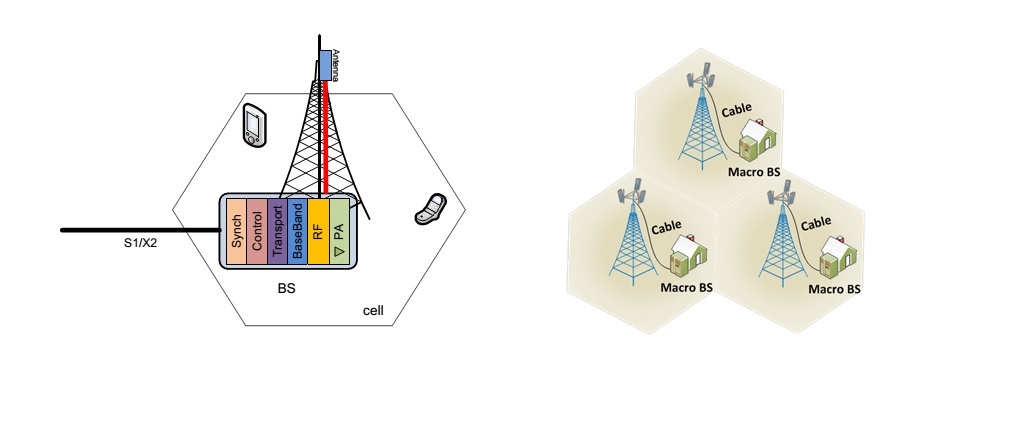
\includegraphics[scale=0.7]{c11}
  \caption{ساختار سنتی ایستگاه پایه \cite{checko2015cloud}}
  \label{fig:c11}
\end{figure}
هر ایستگاه پایه دو نوع پردازش انجام می دهد : پردازش
رادیویی که توسط واحد رادیویی \LTRfootnote{RRH} انجام می شود و شامل پردازش
دیجیتالی، فیلترینگ فرکانسی، تقویت توان و ....میباشد و
پردازش باند پایه که توسط واحد باند پایه \LTRfootnote{BBU} که همان واحد کنترل است \LTRfootnote{CU} انجام شده و از جمله
مهمترین وظایف آن می توان به کدینگ، مدولاسیون و
تبدیل فوریه ی سریع اشاره کرد. در ساختار جدیدی که
تحت عنوان \lr{C-RAN}  معرفی خواهیم نمود نحوه ی ارتباط
پردازشگرهای رادیویی و باند پایه متحول شده و در نتیجه
مزایایی برای شبکه حاصل خواهد شد.در ادامه ، انواع ساختارها را بیان خواهد شد.

\subsection{پیش زمینه ها} 
\subsubsection{ساختار سنتی ایستگاه پایه }

در ساختارهای سنتی ایستگاه پایه، پردازش های رادیویی و باند پایه در
داخل ایستگاه پایه انجام می شد و مدول آنتن نیز در فاصله
ی چند متری از مدول رادیویی نصب شده و ارتباط آنها
توسط کابل کواکسیال برقرار می شد که همین امر سبب
افزایش تلفات در شبکه می باشد. این نوع ساختار در شکل
\ref{fig:c11} نشان داده شده است. همان گونه که مشاهده می کنید
ارتباط بین ایستگاههای پایه توسط ارتباط  $X_2$ و ارتباط بین
ایستگاه پایه و شبکه ی هسته توسط ارتباط $ S_1$ برقرار می
شود. این نوع ساختار در شبکه های \lr{1G} و \lr{2G} به کار گرفته
شده است 
\cite{checko2015cloud}.

%Figure \ref{fig:gull} shows a photograph of a gull.
\subsubsection{ ساختار ایستگاه پایه و واحد رادیویی}

\begin{figure}
  \centering
    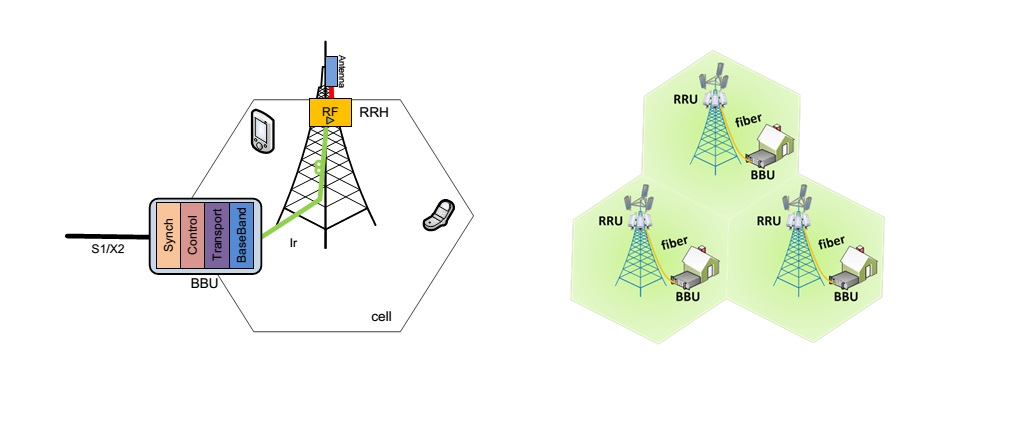
\includegraphics[scale=0.7]{c22}
  \caption{ ساختار ایستگاه پایه و واحد رادیویی \cite{checko2015cloud}}
  \label{fig:c22}
\end{figure}
در این ساختار واحد رادیویی و واحد پردازشی سیگنال، از هم
مجزا شده و واحد رادیویی که تحت عنوان \lr{RRH} یا \lr{RRU}
نیز شناخته می شود، توسط فیبر نوری به واحد باند پایه یا \lr{BBU} اتصال می
یابد. همان طور که پیشتر بیان شد واحد رادیویی مسئولیت
انجام پردازش های دیجیتالی از جمله تبدیل انالوگ به
دیجیتال، دیجیتال به انالوگ، تقویت توان و فیلترینگ رابر عهده دارد، که تفکیک وظایف واحد پردازشی و واحد
رادیویی در این ساختار در شکل \ref{fig:c22} قابل مشاهده است. این
نوع ساختار برای شبکه های نسل سوم معرفی شده و امروزه
نیز بیشتر ایستگاههای پایه از همین ساختار بهره می گیرند.
از جمله ویژگی های بارز این ساختار امکان ایجاد فاصله
بین واحد رادیویی و پردازشی می باشد، که این فاصله به
دلیل تاخیر پردازشی و انتشاری نمی تواند از  $40$کیلومتر
فراتر رود. در این ساختار تجهیزات مرتبط با \lr{BBU} می
توانند به مکانی مناسبتر که قابل دسترس تر بوده و هزینه
ی اجاره و نگهداری کمتری را به اپراتورها تحمیل می
کنند منتقل شوند و واحد های رادیویی نیز در در پشت بام
ساختمان ها و مکان های مرتفع نصب می شوند که این
خود سبب کاهش هزینه های خنک سازی ادوات موجود
می شود. نحوه ی ارتباط بین \lr{RRH} و \lr{BBU} مشابه ساختار
سنتی بوده و \lr{RRH} ها نیز توسط معماری زنجیروار با هم
در ارتباطند.
\begin{figure}[H]
  \centering
    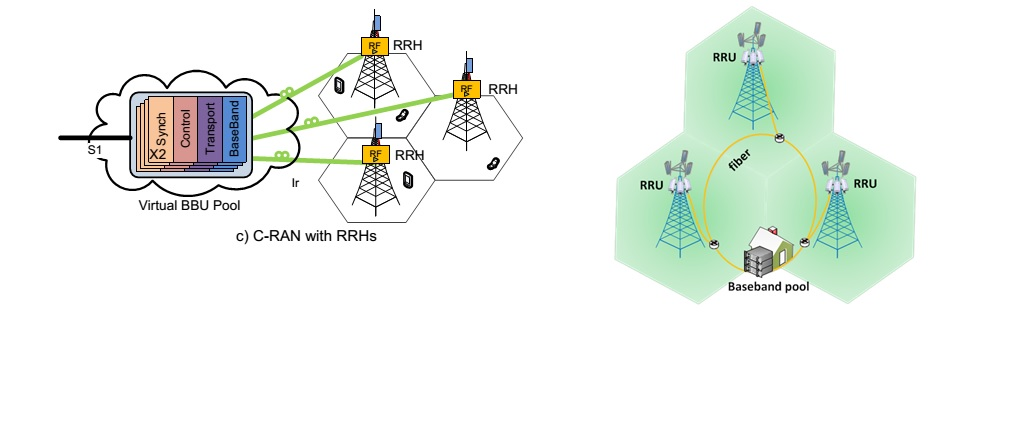
\includegraphics[scale=0.7]{c33}
  \caption{ساختار  \lr{C-RAN} \cite{checko2015cloud}}
  \label{fig:c33}
\end{figure}
\subsection{تعریف مسئله}
\subsubsection{ساختار \lr{C-RAN}}
این ساختار جدید جزو یکی از ساختارهایی است که در \lr{5G} امکان استفاده را دارد.در این ساختار جدید در راستای بهینه سازی عملکرد \lr{BBU}
 ها در مواجهه باایستگاههای پایه پر ترافیک و کم ترافیک،
 \lr{BBU}ها به صورت یک مجموعه ی واحد تحت عنوان 
\lr{BBU Pool}
 در آمده اند که این مجموعه بین چندین سلول 
 به اشتراک گزارده شده و مطابق شکل زیر مجازی سازی
می شود. 
در توضیح بیشتر این ساختار می توان این گونه
عنوان کرد که \lr{BBU Pool} به عنوان یک خوشه ی مجازی
در نظر گرفته می شود که شامل پردازش گرهایی می باشد
که پردازش های باند پایه را انجام می دهند. ارتباط بین
  \lr{BBU}ها در ساختار های فعلی به شکل  $X_2$ برقرار می شود
که در این ساختار ارتباط بین خوشه ها از فرم جدید $X_2$
تحت عنوان  $X_2 +$برقرار می شود.
\newline
در شکل \ref{fig:c33} ساختار کلی شبکه ی  \lr{C-RAN} در سیستم های
\lr{ LTE}
 نمایش داده شده است. همان طور که در شکل قابل
مشاهده می باشد ساختار کلی شبکه  \lr{C-RAN} به دو بخش
 \lr{backhaul} و \lr{fronthaul} تقسیم بندی شده است. بخش
 \lr{fronthaul}شبکه به مرحله ی اتصال سایت های \lr{ RRH}به
 به \lr{BBU Pool} به اتصال \lr{backhaul} و بخش \lr{BBU Pool}
هسته ی شبکه ی سیار اطلاق می شود. همان گونه که قبلا
ذکر شد  \lr{ RRH}ها در نزدیکی انتن نصب شده و از طریق
لینک های انتقالی نوری با پهنای باند وسیع و تاخیر کم به
پردازشگرهای قوی در  \lr{BBU}متصل می شوند. توسط این
لینک های انتقالی است که سیگنال های دیجیتالی باند
پایه از نوع \lr{IQ} بین \lr{RRH} و \lr{BBU} انتقال می یابند \cite{checko2015cloud}.
\begin{figure}[H]
  \centering
    \includegraphics[width=\textwidth]{CRAN}
  \caption{ساختار شبکه ی \lr{C-RAN} \cite{checko2015cloud}}
  \label{fig:C-RAN}
\end{figure}
\section{مزایای شبکه ی \lr{C-RAN}}

در این بخش قصد داریم مزایای شبکه ی \lr{C-RAN} و هدف از استفاده ی آن در \lr{5G} را بیان کنیم.
\newline
در هر دو نوع سلولهای ماکرو و میکرو، می توان از ساختار \lr{C-RAN} بهره برد. در حالت ماکرو، متمرکز کردن \lr{BBU} ها به صورت \lr{BBU Pool}، منجر به استفاده ی بهینه از \lr{BBU} ها و کاهش هزینه ی ایستگاه پایه \LTRfootnote{base station} می شود. همچنین منجر به کاهش مصرف توان و فراهم کردن انعطاف پذیری بیشتر در شبکه و تطبیق آن با ترافیک غیر یکسان می شود. علاوه بر این، باعث تبدیل سیگنال تداخل به سیگنال مفید تبدیل می شود. در ادامه این مزایا به صورت گسترده تر بیان می گردد. \cite{checko2015cloud, namba2012colony}
\begin{figure}
  \centering
    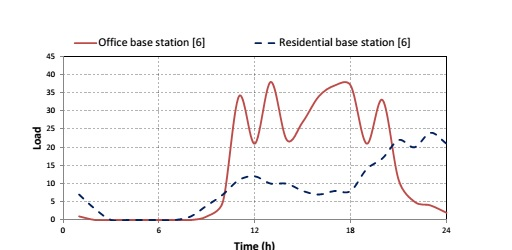
\includegraphics[width=\textwidth]{c4}
  \caption{تغییرات حجم ترافیک در ایستگاههای پایه بنا به
مکان قرارگیری آنها \cite{checko2015cloud}}
  \label{fig:c4}
\end{figure}
\subsection{توانایی تطبیق پذیری با ترافیک غیر
یکنواخت }
کاربران شبکه های رادیویی در طول روز بین مناطق مختلف
(مسکونی و اداری) جابه جا شده و در نتیجه ترافیک هر
منطقه نیز بنا به نوع منطقه در طول ساعات شبانه روز متغیر
می باشد.
نمودار مربوط به این تغییرات در شکل \ref{fig:c4} قابل
مشاهده است. نکته ی قابل توجه برای اپراتور ها در این
بخش، هدر رفت توان پردازشی در اثر جا به جایی کابران می
باشد. بدین شکل که به طور مثال بعد از اتمام ساعات کاری
کاربران شبکه از مناطق اداری به مناطق مسکونی نقل مکان
می کنند حال انکه ایستگاههای پایه برای خدمات رسانی
در اوج ترافیک تعبیه شده و با کاهش تعداد کاربران در
حقیقت توان پردازشی هدر می ر ود. تحقیقات نشان داده
است که میزان پیک ترافیک شبکه حدود  $10$ برابر بیشتر
از ترافیک در ساعات غیر اوج می باشد و در هر سلول بنا
به نوع منطقه ساعات اوج ترافیک متغیر است. با توجه به
متغیر بودن ساعات اوج ترافیک در سلول های مختلف و
با استفاده از ویژگی شبکه های \lr{C-RAN} می توان راهکاری
ارائه نمود که از هدر رفت توان پردازشی جلوگیری شود.
در شبکه های \lr{C-RAN} پردازش های باند پایه مربوط به
چندین سلول به ابر منتقل شده که می توان از این ویژگی
برای افزایش نرخ بهره وری استفاده کرد.  \cite{checko2015cloud, namba2012colony} 
\subsection{صرفه جویی در هزینه و مصرف انرژی }
با بکارگیری شبکه های \lr{C-RAN} در مصرف انرژی و از این
رو در کاهش هزینه ها می توان صرفه جویی نمود.
هزینه
های صورت گرفته توسط اپراتورهای سیستم های مخابراتی
که تحت عنوان \lr{TCO} نیز شناخته می شود،به دو دسته
ی عمده تقسیم بندی می شود. هزینه های \lr{CAPEX} و
هزینه های \lr{OPEX}؛
که هزینه ی \lr{CAPEX} مربوط به ساخت شبکه که شامل طراحی و نصب سخت افزارها می باشد. هزینه ی \lr{OPEX} شامل هزینه های مربوط به راه اندازی و نگهداری وهمچنین
ارتقای شبکه ی مخابراتی می باشد. که \lr{C-RAN} منجر به کاهش هر دو هزینه می شود.
\subsection{سهولت در ارتقا دادن و نگهداری از شبکه}
با قرار گیری  \lr{ BBU} ها در داخل ابر به جای قرارگیری در
ایستگاه های پایه ی دور از هم امکانسهولت در ارتقا دادن و نگهداری از شبکه در صورت نیاز به مداخله ی نیروی انسانی
فراهم می شود، زیرا در این صورت به جای نظارت بر تمام
ایستگاههای پایه تنها تعداد مشخصی \lr{BBU pool} مد نظر
قرار می گیرند. هم چنین بروزرسانی \lr{CPU} در این حالت
تسریع شده و استفاده از تکنولوژی \lr{IT} به جای استفاده از
سخت افزارها هموارتر می شود.
\begin{figure}
  \centering
    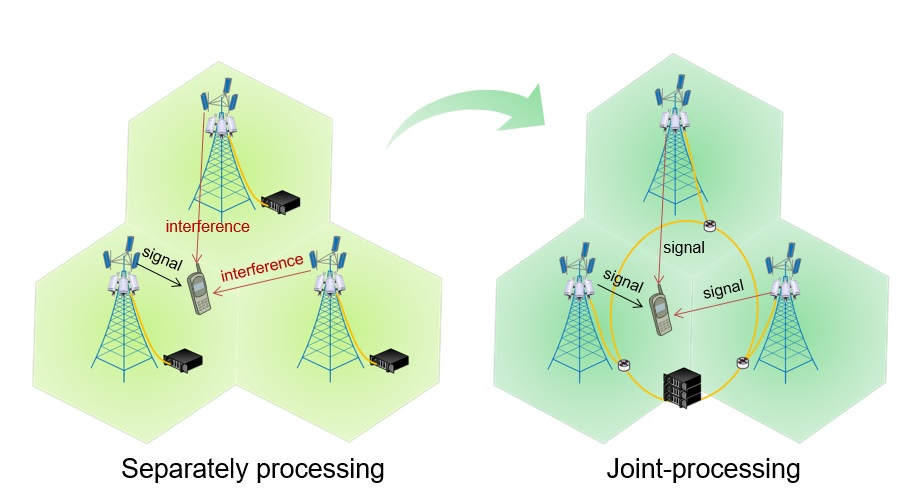
\includegraphics[width=\textwidth]{c55}
  \caption{تداخل در \lr{LTE} و \lr{C-RAN} \cite{WinNT}}
  \label{fig:c55}
\end{figure}
\subsection{کاهش چشمگیر تداخل از طریق پردازش واحد باند پایه }
تداخل در شهرهای بزرگ یکی از چالشهای مهم محسوب می شود. \newline
همانطور که در شکل \ref{fig:c55} دیده می شود، در \lr{LTE} تداخل به صورت واضحی بر روی سیگنال مفید اثر می گذارد، حال در \lr{C-RAN} این مشکل به صورتی که در شکل دیده می شود برطرف شده و سیگنال تداخل تبدیل به سیگنال مفید می شود و از رابطه ی متقابل کانال \lr{TDD} \LTRfootnote{Time Division Duplexing} استفاده می گردد.

\subsection{افزایش توان و کاهش تاخیر}
در سالهای اخیر شبکه های نسل $4$  یا \lr{LTE} توسط \lr{ 3GPP}
استاندارد سازی شده و به مرور جایگزین سیستم های نسل $3$
 شده اند.
 
  شبکه های \lr{C-RAN} 
 با توجه به قابلیت هایی
که دارند در سیستم های نسل $4$ یعنی \lr{LTE} و \lr{LTE-A}
قابل پیاده سازی و بهره برداری بوده و مزایایی را برای این
سیستم ها به همراه خواهند داشت. برای توضیح بهتر نقش
   \lr {C-RAN} در افزایش توان عملیاتی نیاز هست که با تکنیک
هایی از قبیل  \lr{eICIC} و  \lr{CoMP} اشنا شده و سپس این
تکنیک ها را به ساختار \lr{C-RAN} تعمیم بدهیم.
همان طور که می دانید در سیستم های \lr{LTE} منابع به
صورت مشارکتی مورد استفاده قرار می گیرند. مسئولیت
تخصیص منابع در این شبکه ها به عهده ی زمانبندی 
به نام \lr{eNB} \LTRfootnote{eNode B} است که در ایستگاه پایه قرار دارد. نکته ی
قابل توجه دیگر استفاده از تکنیک \lr{OFDMA} می باشد که
زمانبند را قادر می سازد که منابع را به صورت دینامیکی
هم در حوزه ی زمان و هم در حوزه ی فرکانس به کاربران
مختلف تخصیص دهد.
با توجه به این که در سیستمهای \lr{ LTE} عموما پارامتر استفاده
ی مجدد از فرکانس برای تمامی سلول ها یک در نظر
گرفته می شود، در نتیجه تداخل بین سلول های مجاور
به شدت افزایش می یابد. برای رفع این مشکل دو روش
عمده مطرح می شود: روش اول کاهش تداخل و روش دوم
استفاده ی سازنده از تداخل. برای پیاده سازی روش اول
از تکنیک \lr{ICIC} یا \lr{eICIC} استفاده می شود و برای روش
دوم عمدتا از تکنیک \lr{CoMP} بهره می گیرند که توضیح
نحوه ی عملکرد این تکنیک ها در مقاله ها به طور کامل
بررسی شده است. در رابطه با کاهش تاخیر نیز می توان
این گونه عنوان نمود که با قرار گرفتن \lr{ BBU} ها در مجاورت
هم در ابر مدت زمان لازم برای انجام عمل \lr{hand off} بین
ایستگاههای پایه کاهش می یابد. زیرا عمل\lr{hand off} در
این حالت به جای ایستگاههای پایه در \lr{ BBU} ها صورت
می گیرد
\section{چالشها و مشکلات در برخورد با ساختار \lr{C-RAN} }

\subsection{دو چالش مهم مربوط به \lr{fronthaul}}
 \begin{figure}
  \centering
    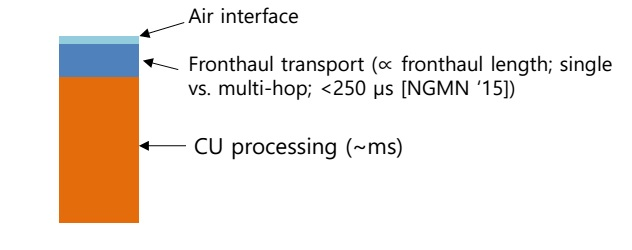
\includegraphics[scale=0.7]{c6}
  \caption{محدودیت در اثر تاخیر \cite{simeoneConf}  }
  \label{fig:c6}
\end{figure}
یکی از مشکلات پیش روی ساختار \lr{C-RAN} در قسمت \lr{fronthaul} به شرح زیر است.
\begin{itemize}
\item
 محدودیت ظرفیت که
 به دو دلیل ایجاد می گردد که در ادامه ذکر شده است \cite{simeoneConf}.
 \begin{itemize}
 \item
 نمونه برداری و کوانتیزاسیون اسکالر
 \item
 تداخل رادیویی به صورت عمومی
 \end{itemize}
  
 \item 
  محدودیت در اثر تاخیر که
   به سه دلیل ایجاد می شود که در ادامه ذکر شده است \cite{simeoneConf}.
  \begin{itemize}
 \item
 تداخل هوا
 \item
 انتقال سیگنال در قسمت \lr{fronthaul}
 \item
 پردازش واحد کنترل
 \end{itemize}
   انتقال سیگنال در قسمت \lr{fronthaul} و پردازش واحد کنتذل به نوع انتقال \lr{fronthaul} بستگی دارد (بسیم یا انتقال با سیم) 
\end{itemize}
با استفاده ازمخابرات فیبر نوری این مشکلات تا مقدار زیادی حل خواهد شد. 
\subsection{نحوه ی مشارکت \lr{BBU} ها نحوه ی اتصال
و خوشه بندی}

همکاری بین ایستگاههای پایه بایستی به گونه ای باشد
که از نظر زمانبندی و بررسی اطلاعات بازخورد کانالها
به منظور مدیریت تداخل و همچنین سازگاری باتکنیک
   \lr{CoMP}مورد بررسی قرار گرفته باشد.
تکنیک هایی که برای اتصال \lr{BBU}ها مورد استفاده قرار
می گیرند بایستی از نظر امنیت، قابلیت اطمینان، پشتیبانی
از پهنای باند وسیع ،تاخیر کم و ... استاندارد های لازم را
براورده ساخته و نسبت به ساختار سنتی عملکرد بهتری را
از خود نشان دهند.
\subsection{نیاز به پهنای باند وسیعتر و تاخیر
دقیق و کمتر}
در ساختار شبکه ی \lr{C-RAN} اطلاعات به صورت \lr{ IQ} بین
 \lr{RRH} و  \lr{BBU} ها انتقال می یابند. طبق استانداردهایی
که برای این شبکه تعریف شده است، انتظار می رود که
هر \lr{BBU pool} قابلیت خدمات دهی به $100-1000$
ایستگاه پایه را دارا باشد. بنابراین با توجه به پهنای
باند مورد نیاز برای ارسال اطلاعات به صورت \lr{ IQ} حجم
اطلاعاتی زیادی توسط لینک های نوری به سمت \lr{BBU pool}
  ها سرازیر خواهد شد و پهنای باند بالایی مورد نیاز
است.علاوه بر نیاز به پهنای باند بالا شبکه ی انتقال ما
بایستی نیاز به جیتر و تاخیر دقیق در شبکه را برآورده کند،
که در ادامه برخی از این قیود لازم آورده شده است.
\begin{itemize}
\item
دقت زمانی لازم برای همکاری بین ایستگاههای پایه
بایستی در حدود $ 0.5 \mu sec$ باشد که مهم ترین شرط
این مبحث محسوب می شود.
\item
صرف نظر از تاخیر حاصل از طول
کابل تاخیر حاصل از رفت و برگشت اطلاعات کاربران
نبایستی از حدود $ 5 \mu sec$ بیشتر باشد
\item
فاصله ی بین \lr{RRH} و \lr{BBU} ها بایستی از حد 
 $ 20 - 40 km$تجاوز نکند و تاخیر حاصل از پردازش زیر
 فریم ها در لینک های ارتباطی بین  \lr{RRH} و \lr{BBU} نیز
بایستی از $1ms$ کمتر باشد
\end{itemize}
\subsection{محدودیت ظرفیت در \lr{backhaul}}
همچنین محدودیت ظرفیت در \lr{backhaul} منجر به محدود کردن عملکرد انتقال در حالت مشارکت چند نقطه ای  در  \lr {C-RAN} می گردد. 
\subsection{نیاز به شبکه های انتقال ازران}
برای انتقال اطلاعات بین \lr{RRH} و \lr{BBU} از فیبر نوری
استفاده می شود. فیبر نوری به دلیل سرعت در انتقال
اطلاعات تلفات کم و قابلیت انتقال حجم بالایی از
اطلاعات گزینه ی مناسبی برای شبکه های \lr{C-RAN} به
حساب می اید. با وجود محاسن گفته شده گران بودن و
عدم دسترسی تمام اپراتورها به فیبر نوری از جمله مشکلاتی
است که بایستی قبل از پیاده سازی شبکه های \lr{C-RAN} بدان
پرداخته شود. \cite{MA}
\section{شبکه های دسترسی رادیویی ابری نا متجانس (\lr{H-CRAN})}
برای غلبه بر چالش های شبکه های \lr{C-RAN} با محدودیت های \lr{fronthaul} ، شبکه های دسترسی ابری نامتحانس (\lr{H-CRAN}) معرفی گردید\cite{ fogComputing, heterogeneous, fogEdge}.
\begin{figure}
  \centering
    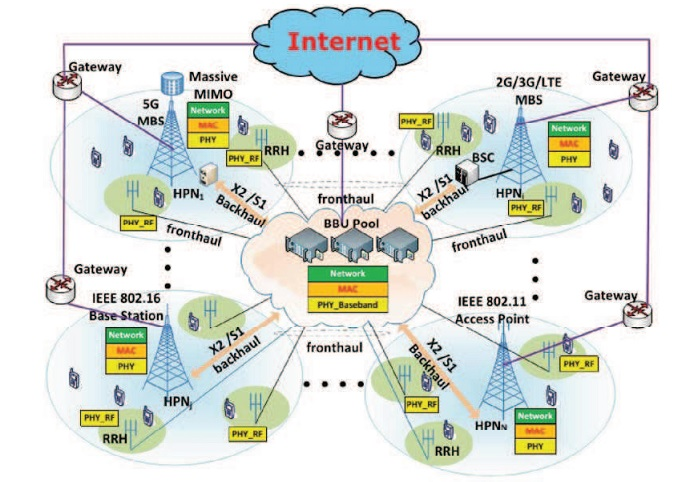
\includegraphics[scale = 0.8]{hc}
  \caption{ ساختار شبکه های دسترسی ابری نامتحانس \cite{heterogeneous}  }
  \label{fig:hc}
\end{figure}

\subsection{ساختار شبکه ی \lr{H-CRAN}}
کاربر و صفحه ی کنترلگر در چنین شبکه هایی از هم مجزا می باشند. که در این شبکه ها ، نودهای توان بالا   \LTRfootnote{High Power Node}\lr{HPN} ، عمدتا برای فراهم کردن پوشش بدون درز و اجرای عملکرد صفحه کنترل می باشد. در حالی که \lr{RRH} ها برای فراهم نمودن سرعت بالای نرخ داده برای انتقال بسته در ترافیک قرار گرفته اند. \lr{HPN} ها از طریق لینکهای \lr{backhaul}  به \lr{BBU Pool} متصلند ( برای هماهنگ کردن تداخل ).\newline
ساختار این شبکه شبیه به ساختار \lr{C-RAN} می باشد . همانطور که در شکل \eqref{fig:hc} نشان داده شده است ، تعداد زیادی \lr{RRH} ، همراه با انرژی مصرفی کم در ساختار \lr{H-CRAN} ، با یکدیگر در \lr{BBU Pool} مرکزی ، همکاری می کنند تا گین مشترک بالایی بدست آورند.   تنها ، فرکانس رادیویی جلو ،(\lr{RF}) و عملکردهای پردازشی  ساده ، در \lr{RRH} ، صورت می گیرد ، در حالی که پردازشهای مهم دیگر ، در \lr{BBU Pool} انجام می گیرد. همچنین تنها بخشی از عملکردها در لایه ی \lr{PHY} در \lr{RRH} به مشارکت می انجامد که این مدل در شکل \eqref{fig:hc} نشان داده شده است.\newline
اگرچه ، برخلاف \lr{C-RAN} ، \lr{BBU Pool} در \lr{H-CRAN} ، به \lr{HPN} ها متصلند که این، برای کاهش تداخل متقابل بین \lr{RRH} ها و \lr{HPN} ها از طریق محاسبات ابری متمرکز بر اساس تکنیکهای پردازشی مشترک می باشد. همچنین ، داده و واسط کنترل ، بین \lr{BBU Pool} و \lr{HPN} های $S_1$ و $X_2$ شناخته شده اند که تعریف آنها بر اساس تعریف استاندارد \lr{3G} ایجاد شده است.\newline
همانطور که سرویسهای صدا ، می توانند به صورت بهینه در طول مد سوییچ بسته در \lr{4G} فراهم گردند ، \lr{H-CRAN} می تواند به طور همزمان سرویس صدا و داده را پشتیبانی کند. سرویس صدا مرجح به اداره از طریق \lr{HPN} ها می باشد ، در حالی که ترافیک بسته ی پر داده ، بیشتر توسط \lr{RRH} اداره می گردد. 
در مقایسه با ساختار \lr{C-RAN} ،ساختار \lr{H-CRAN} ، نیازهای \lr{fronthaul} را بوسیله ی مشارکت \lr{HPN} ها برطرف می سازد. با توجه به حضور \lr{HPN} ها ،سیگنالهای کنترلی و سمبلهای داده در \lr{H-CRAN} جدا از هم می باشند. تمام کنترل کننده های سیگنال و سیستم هایی که اطلاعات را ارسال می نمایند ، توسط \lr{HPN} ها به \lr{UE} ، منتقل می گردد که منجر به سادگی در ظرفیت و در محدودیت تاخیر زمان در لینکهای \lr{fronthaul } بین \lr{RRH} ها و \lr{BBU Pool}  می گردد و منجر به صرفه جویی در مصرف انرژی می گردد. همچنین ، برخی از ترافیک های شدید و ناگهانی \LTRfootnote{Burst Traffic} و یا سرویس پیام همراه با مقدار داده ی کم ، می تواند به صورت بهینه توسط \lr{HPN} ها پشتیبانی گردد. مکانیزم کنترل بین ارتباط داشتن و نبود ارتباط ، توسط \lr{H-CRAN} پشتیبانی می گردد که منجر به حفظ کردن مقدار قابل توجهی \lr{Overhead} در رادیو بوسیله ی مکانیزم ارتباط جهت دار خالص می گردد. در \lr{RRH} ، تکنولوژی های مختلف انتقال در لایه ی \lr{PHY} ، قابل استفاده برای بهبود نرخ انتقال (همانند موج میلیمتری و نور مرئی) می گردد. در \lr{HPN}ها، \lr{MIMO}\LTRfootnote{Multiple Input Multiple Output}، یکی از راه های افزایش پوشش در بهبود ظرفیت می باشد.

\subsection{چالشهای پیش روی \lr{H-CRAN}}
متاسفانه ، \lr{H-CRAN} در عمل دچار چالشهایی است.
\begin{itemize}
\item
 اولین چالش به این دلیل است که با معروفتر شدن موقعیتهایی که بر اساس کاربردهای اجتماعی است ، داده های ترافیکی در طول مسیر  \lr{fronthaul} از \lr{RRH} به \lr{BBU Pool}، با افزایش موج زیادی از داده های زائد همراه است که منجر به بدتر شدن محدودیت \lr{fronthaul} می گردد.
\item
همچنین \lr{H-CRAN} ، از تمامی فواید پردازشی و ظرفیت ذخیره در ابزارهای پردازشی و الکترونیکی همانند \lr{RRH} و تلفن های هوشمند (\lr{UE}) ،که راه های رسیدن به موفقیت در این ساختار است ، استفاده نمی کند .
\item
همچنین ، اپراتورها ،نیاز به استقرار تعداد زیادی \lr{RRH} و \lr{HPN} ثابت در \lr{H-CRAN} ، می باشند تا به ماکسیمم ظرفیت دسترسی پیدا کنند. ولی در زمانهایی مه ترافیک زیاد نیست ، منجر به اتلاف شدیدی می شود. 
\end{itemize}
\section{\lr{C-RAN}و \lr{H-CRAN} }

\subsection{تفاوت و شباهت های این دو ساختار}
  تفاوت عمده ی بین این دو ساختار در این است که در \lr{H-CRAN} ، عملگر کنترل مرکزی از \lr{BBU Pool} به \lr{HPN} منتقل گردیده است. \cite{fogComputing}
 \newline
در هر دو ساختار، عملگرهای \lr{CRSP} \LTRfootnote{Collaboration Radio Signal Processing} و ذخیره سازی اطلاعات در سرور ابر مرکزی ، صورت می گیرد که نیاز به تعداد زیادی دستگاه های فرستنده (موبایل) و انتقال داده به سرعت کافی از طریق \lr{BBU Pool} می باشد.
\subsection{مشکلات پیش روی این دو ساختار}
مهمترین مشکلات این دو ساختار ، تاخیر انتقال زیاد و سنگینی حمل اطلاعات بر روی \lr{fronthaul} می باشد.روش ساده یرای حل این مشکل :
\begin{itemize}
\item
جلوگیری از انتقال تمام داده ها به \lr{BBU Pool} شویم و بخشی از پردازش اطلاعات را در \lr{RRH} های محلی و همچنین وسایل الکترونیکی هوشمند انجام دهیم.
\item
جلوگیری کنیم از اینکه همه ی ترافیک به طور مستقیم از سرور ابر متمرکز منتقل شود، برخی از ترافیک محلی باید از ذخیره  \lr{RRH} های مجاور تحویل گردد.
\end{itemize}
\section{ارائه ی پیشنهاد سیستم جایگزین (\lr{F-RAN})}
برای حل کردن مشکلات \lr{H-CRAN} و \lr{C-RAN}، نیاز به معرفی ساختار جدید دیگری می باشیم که آن را \lr{F-RAN} می نامیم.
\lr{F-RAN} تمام ویژگی های مثبت محاسبات ابری و شبکه های نامتجانس و محاسبات مهی را همزمان در بر می گیرد.
محاسبات مهی ، اصطلاحی برای جایگزین کردن محاسبات ابری است که مقدار قابل توجهی از ذخیره سازی ، ارتباطات ، کنترل کردن ، اندازه گیری و مدیریت را در لبه ی شبکه انجام می دهد (نه در کانال و ابر مرکزی) \cite{fogComputing, fogEdge,fog12}.
\begin{figure}
  \centering
    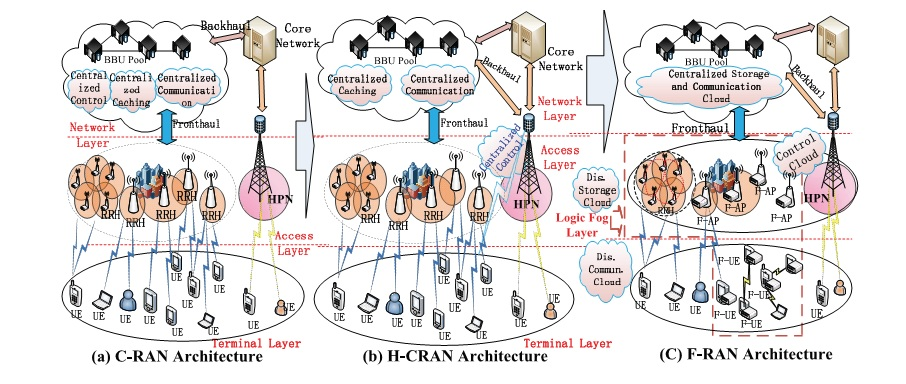
\includegraphics[scale = 0.7]{fhc}
  \caption{ سیر تحولات شبکه های رادیویی ابری \cite{fogComputing}}
  \label{fig:fhc}
\end{figure}
\subsection{ساختار سیستمهای   \lr{F-RAN}}
 سیستمهای \lr{F-RAN} تحولی از سیستمهای \lr{C-RAN} می باشد که در شکل \eqref{fig:fhc} نشان داده شده است. برخی از ارتباطات توزیع شده و عملکردهای ذخیره سازی در منطق لایه ی مه قرار دارد. همچنین چهار نوع ارتباطات ابری تعریف شده است.
  \begin{figure}[H]
  \centering
    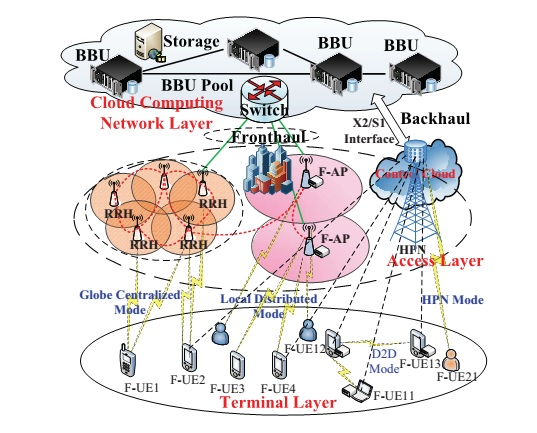
\includegraphics[scale =0.7]{fr}
  \caption{ مدل سیستم \lr{F-RAN} \cite{fogComputing} }
  \label{fig:fr}
\end{figure}
 \begin{itemize}
 \item
 ابر ذخیره گر و ارتباطات مرکزی جامع :
 که همانند ابر مرکزی \lr{C-RAN} می باشد
 \item
 ابر کنترل گر مرکزی :که برای تکمیل عملکردهای کنترلی  می باشد و در \lr{HPN} ها قرار دارد
 \item
 ابر ارتباطات منطقی توزیع شده که در برنامه های محاسبات مهی و ابزار های این محاسبات قرار دارد.
 \item
  ابر ذخیره گر منطق توزیع شده:
  که همانند قبل در \lr{F-RAN} قرار دارد.
 \end{itemize}
 در این ساختار ، برای کاهش تاخیر ناشی از انتقال داده ها به ابر مرکزی ، ساختار های \lr{RRH} را دارای حافظه قرار می دهیم که برای ارتباطات محلی، به جای اینکه پردازش ها در \lr{BBU Pool} صورت بگیرد، بدون نیاز به انتقال به ابر مرکزی، درون \lr{RRH} ها انجام پذیرد. 
 %%%%%%%%%%%%%%%%%%%%%%%5
 %%%%%%%%%%%%%%%%%%%%%%%
 \section{برخی از کاربردهای شبکه ی \lr{C-RAN}  }

\subsection{ تخصیص منابع مبتنی بر مدولاسیون \lr{OFDM}}
هدف از متد ارائه شده در برخی مقالات را می توان تخصیص
منابع بین سلول ها با در نظر گرفتن تداخل بین سلول و هم
چنین کاهش تعداد \lr{BBU} های فعال عنوان کرد. نحوه ی
تخصیص به  ۲بخش تقسیم شده و به طور جداگانه بررسی
شده است. بخش اول و اصلی تخصیص منابع بین ناحیه
های لبه سلول ها می باشد که بایستی تداخل در نظر گرفته
شده و بدان منظور از روش \lr{graph coloring} استفاده شده
است و بخش دوم تخصیص منابع بین ناحیه های مرکزی
می باشد که بنا به تخصیص های صورت گرفته در بخش
اول انجام می شود. در ادامه عملکرد متد ارائه شده برای
تخصیص منابع مبتنی بر شبکه \lr{C-RAN} بررسی شده و مورد
ارزیابی قرار می گیرد.
در سناریو مورد نظر شبکه ای شامل  ۹سلول در نظر گرفته
و پهنای باندی که که به هر \lr{BBU} تخصیص داده می
شود را برابر $ B = 20MHZ$ در نظر گرفته و تابع توزیع
احتمال ترافیک شبکه را نیز گوسی در نظر می گیریم. دو
پارامتر $\sigma_ck$ و $\sigma_ek$به ترتیب نشانگر پهنای باند مورد نیاز ناحیه
ی لبه و ناحیه ی مرکزی سلول  می باشند. پهنای باند
مورد نیاز به صورت مستقل و یکسان بین تمام سلولها توزیع
شده است .\cite{graph}
\begin{figure}
  \centering
    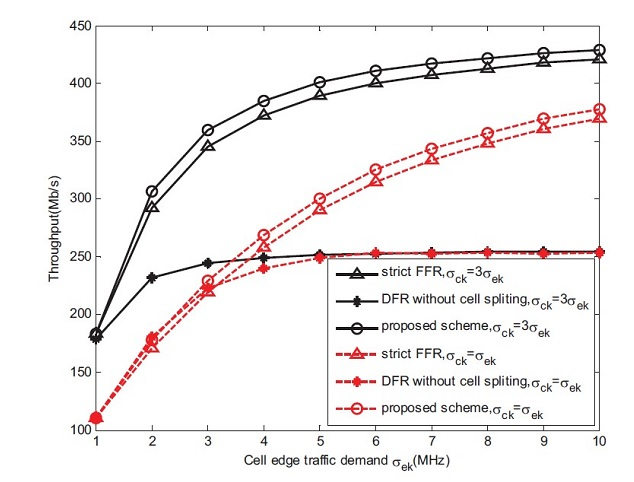
\includegraphics[scale =0.7]{cr}
  \caption{ توان عملیاتی تمام کاربران سلول \cite{graph} }
  \label{fig:cr}
\end{figure}
در شکل \eqref{fig:cr}  توان عملیاتی تمام کاربران سلول چه کاربران
نواحی مرکزی یا لبه مورد بررسی قرار گرفته است. در این
 دو دسته نمودار حاصل می
نمودار با انتخاب  $\frac{\sigma_ck}{\sigma_ek} = \frac{1}{3}$ 
شود که وابستگی عملکرد به تغییرات ترافیک را نشان می
دهند. در نمودار های مذکور متد جدیدی تحت عنوان \lr{DFR} بدون تجزیه ی سلول نیز مشاهده می شود که نحوه
ی تخصیص مطابق روش ارایه شده ما می باشد با این
تفاوت که نواحی لبه و مرکزی تفکیک نشده و کل سلول
واحد در نظر گرفته شده است. با هر دو انتخاب ممکن برای
نسبت ترافیک ها می توان مشاهده کرد که متد ما عملکرد
بهتری را از خود به نمایش می گذارد. متد   \lr{DFR} بدون
تفکیک سلول نیز بدترین عملکرد را از خود نشان می دهد
زیرا نمی تواند به طور بهینه از منابع استفاده کند
در شکل های \eqref{fig:7} و \eqref{fig:8} نیز عملکرد بهره وری انرژی هر ۳
متد مورد نقد و بررسی قرار گرفته است. شایان ذکر است
که میزان بهره وری انرژی به نسبت توان عملیاتی تمام
کاربران به توان تمام \lr{BBU} های فعال اطلاق می شود. با
توجه به نمودار ها بدترین عملکرد متعلق به روش \lr{FFR}
معمول می باشد زیرا به ازای هر سلول از یک  \lr{BBU}مجزا
استفاده می شود.
نکته ی قابل توجه در این نمودار عملکرد
بهتر متد \lr{DFR} بدون تفکیک سلول نسبت به متد ارائه شده
است .علت این امر نیز استفاده از  \lr{BBU}ها ی کمتر از
$\frac{M}{3}$
می باشد. هر چند اگر ما تعداد کمتری کاربر در هر سلول داشته
باشیم و حجم ترافیکی کاهش یابد، نتایج حاصل از متد ارایه
شده از متد \lr{DFR} بدون تفکیک سلول پیشی گرفته و بهترین
عملکرد را از خود نشان می دهد که نتایج مذکور در شکل
  \eqref{fig:8}
   قابل مشاهده است. در این نمودار فرض
\begin{equation*}
\sigma_e k = \sigma_c k
\end{equation*}  
 رعایت شده و میزان $\sigma_ek$ بین  0.2 و 2 انتخاب می شود
با مفروضات انجام شده تعداد \lr{BBU} های فعال در هر دو
متد یکسان شده و چون توان عملیاتی کاربران در متد ارائه
شده بهتر است پس متد مذکور در این نمودار نیز بهترین
عملکرد را نسبت به  2متد دیگر از خود نشان می دهد.  
\begin{figure}
  \centering
    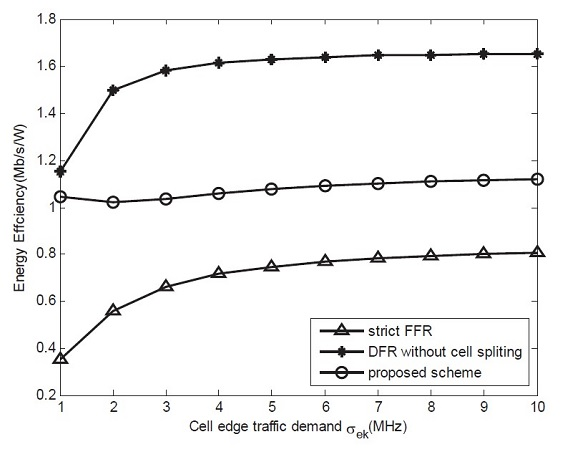
\includegraphics[scale=0.7]{7}
  \caption{ بهره وری انرژی در حضور ترافیک معمول \cite{graph}  }
  \label{fig:7}
\end{figure}

\begin{figure}
  \centering
    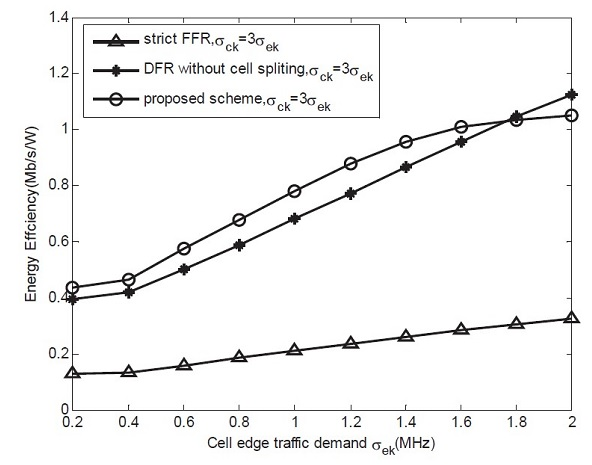
\includegraphics[scale=0.7]{8}
  \caption{  بهره وری انرژی در حضور ترافیک محدود \cite{graph} }
  \label{fig:8}
\end{figure}
\section{تخصیص توان و خوشه بندی شبکه های رادیویی ابری}
برای کاهش پیچیدگی این نوع شبکه ها ، می توان از تکنیک های خوشه بندی در طراحی و چینش\lr{RRH} ها استفاده کرد. برای بهبود بازدهی انرژی و توان نیز می توان تخصیص توان و خوشه بندی شبکه های رادیویی ابری را همزمان با هم انجام داد. 
که این مبحث یکی از بحث های داغ در شبکه های رادیوی ابری می باشد که با روش های بهینه سازی به طور همزمان به تخصیص توان و بدست آوردن تعداد خوشه ها خواهیم رسید .
حتی برای خوشه بندی به طور تنها نیز می توان از روش \lr{K Means} استفاده کرد . در شکل \ref{fig:88} نموداری از نسبت خطا به تعداد  \lr{RRH} در هر خوشه رسم شده است. 
\begin{figure}
  \centering
    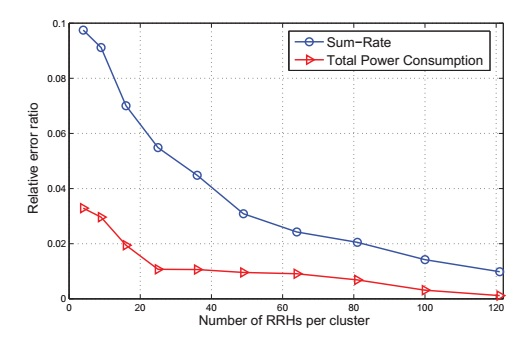
\includegraphics[scale=0.7]{88}
  \caption{  نسبت خطا به تعداد \lr{RRH} در هر خوشه \cite{graph}  }
  \label{fig:88}
\end{figure}
\section{نتیجه گیری}
در این فصل، نسل پنجم مخابرات یعنی \lr{5G} و ساختار جدید \lr{C-RAN} که مورد توجه در این نسل مخابرات است ،مورد بررسی قرار گرفته شده و مزایا و چالش های پیش روی آن به طور مختصری بیان کرده ایم . همچنین ساختار های جدیدی که ساختارهای تعمیم یافته ی \lr{C-RAN}می باشد را مورد بررسی قرار داده ایم.این ساختارهای جدید قابلیت کاهش هزینه های ساخت و بهره
برداری از شبکه و هم چنین بهبود کارایی سیستم از لحاظ
پوشش دهی و تحرک پذیری را دارا می باشد و شاید بتوان
افزایش بهره ی انرژی را جزو مهمترین مزایای این ساختار
عنوان کرد. 


\section{خلاصه ای از فصلهای آتی}
در فصلهای بعدی، مدل سیستم ساختار \lr{C-RAN} مورد بررسی قرار می گیرد.
در فصل 2 به کارهای گذاشته و مدل سیستمهای گذشته در لینک فروسو و فراسو می پردازیم و مفهومی به نام بازدهی انرژی\LTRfootnote{Energy efficiency}
را بیان می کنیم و هدفمان در این فصول بیشینه سازی مجموع نرخ های قابل دسترس و بیشینه سازی بازدهی انرژی می باشد.
در فصل سوم به بررسی مدل سیستم جدیدی می پردازیم که نسبت کارهای قبلی تغییرات اندکی کرده است و در فصل چهارم نیز مدل سیستمی با تغییرات بیشتری را در نظر داریم و در نهایت در فصل پنجم به نتیجه گیری تمام فصل ها پرداخته می شود.






 \chapter{ در ساختار دسترسی رادیویی ابری‌ادبیات و پیشینه ی تحقیق}
 \section{مقدمه}
 شبکه های دسترسی رادیویی ابری، می تواند ساختار جدیدی برای نسل بعدی سیستمهای مخابراتی سلولی باشد. در این ساختار، پردازش های بخش باند پایه از ایستگاه پایه \LTRfootnote{BS}، به واحد کنترل \LTRfootnote{CU} در داخل ابر \LTRfootnote{cloud} منتقل می گردد. ایستگاه باند پایه که به عنوان واحد رادیویی \LTRfootnote{RRH} عمل می کند، توسط لینک \lr{fronthaul}، به واحد کنترل متصل می گردد. لینک \lr{fronthaul}، اطلاعاتی در مورد سیگنالهای باند پایه که در حالت فراسو از واحد رادیویی به واحد کنترل و در حالت فروسو به صورت برعکس ، منتقل می کند. بدلیل محدودیت در ظرفیت لینک \lr{fronthaul}،\cite{fc} اطلاعات قبل از عبور از این لینک، کوانتیزه می گردد.
 %%%%%%%%%%%%%%%%%%%%%%%%%%
 
 
در حال حاضر بسیاری از تحقیقات در زمینه ی \lr{5G} در مورد سیستم های \lr{MIMO} است که در زیرساخت \lr{C-RAN} می باشد.
در این فصل، برخی از نتایج ارائه شده مرتبط با شبکه های دسترسی رادیویی ابری در لینک فروسو و  فراسو بیان می گردد.
\section{لینک فروسو}
در این قسمت، سیستمهای  \lr{MIMO C-RAN} در حالت فروسو مورد بررسی قرار می گیرد. در حالت فروسو،  واحد کنترل، پردازش اطلاعات پیام را با عملکرد کدگذاری کانال و پیش کد گذاری \LTRfootnote{precoding} مدیریت می نماید.
\subsection{مدل سیستم اول}
سیگنال پیش کدگذاری شده ی باند پایه در واحد کنترل، فشرده گشته و توسط لینک ارتباطی \lr{fronthaul} که دارای ظرفیت محدود است \cite{fc2}، به واحد رادیویی منتقل می گردد.
هر واحد رادیویی، از لینک \lr{fronthaul} سیگنالی را که دارای نویز کوانتیزاسیون است، دریافت می کند؛ سپس با اعمال \lr{pulse shaping}، سیگنال را به فرکانس بالاتر منتقل کرده و از طریق کانال بدون سیم به کاربران ارسال می نماید.
\begin{figure}[H]
  \centering
    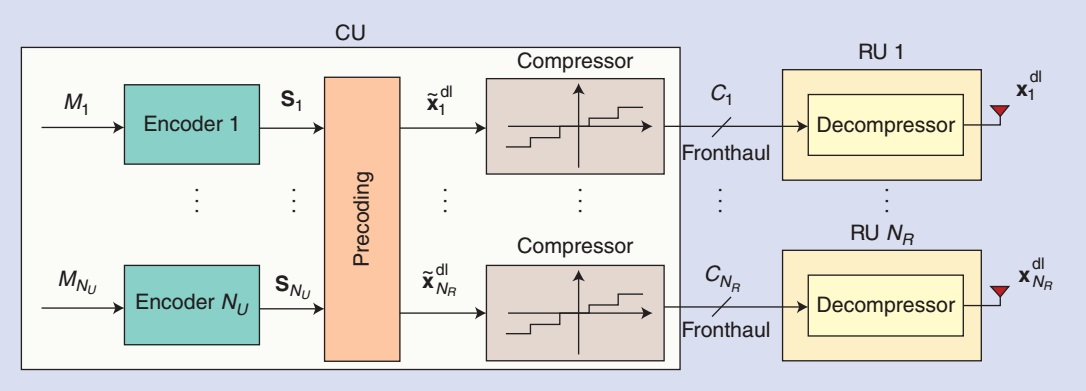
\includegraphics[width=\linewidth, height=6cm]{dl}
  \caption{مسیر انتقال پیام در لینک فروسو \cite{Fronthaul}.}
  \label{fig:dl}
\end{figure}
بلوک دیاگرام مدل سیستم اول
در شکل \ref{fig:dl} نشان شده است. 
در اینجا، $N_U$ کاربر قرار دارند که توسط $N_R$ واحد رادیویی سرویس دهی می شوند.


برای بدست آوردن سیگنال 
$\tilde{\boldsymbol{x}}^{dl}$ ،
واحد کنترل، سیگنال پیام را به صورت مجزا برای هر کاربر کدگذاری می کند.  با  اعمال این فرآیند،  سمبلهای $\boldsymbol{s}=[s_1;...;s_{N_U}]$  بدست می آید که $s_k$ نشان دهنده ی سمبل $k$ امین کاربر می باشد. 
سیگنال پیش کدگذاری شده ی
$\tilde{\boldsymbol{x}}^{dl} $
که توسط واحد کنترل تولید می گردد به این صورت بیان می شود:
\begin{equation}\label{wp}
 \tilde{\boldsymbol{x}}^{dl} = \boldsymbol{W}\boldsymbol{P}^{\frac{1}{2}} \boldsymbol{s},
\end{equation}
که 
 \begin{equation}
\tilde{\boldsymbol{x}}^{dl} = [\tilde{x}_{1}^{dl}; ... ; \tilde{x}_{N_R}^{dl}] 
 \end{equation}
 در رابطه ی  \eqref{wp}، $\boldsymbol{W}$، ماتریس پیش کدگذاری شده با ابعاد $N_R \times N_U$ می باشد و $\boldsymbol{W} = [\boldsymbol{w_1},..., \boldsymbol{w_{N_{U}}}]$ است. علاوه بر این، 
 $\boldsymbol{P}^{\frac{1}{2}} = diag(\sqrt{p_1},...,\sqrt{p_{N_U}})$ 
 ماتریس توان است.
حال سیگنال فشرده شده ی دریافتی توسط واحد رادیویی به صورت زیر بدست می آید:
\begin{equation}
\label{eq_pow1}
 {\boldsymbol{x}}^{dl} = \tilde{\boldsymbol{x}}^{dl} + \boldsymbol{Q},
\end{equation}
که در اینجا $\boldsymbol{Q} = \left[ q_1,\ldots,q_{N_R}\right]^T$، بردار نویز کوانتیزاسیون تولید شده به دلیل فشرده سازی بعد از پیش کدگذاری در واحد کنترل می باشد که دارای توزیع 
 $ \forall i  \quad  q_i\backsim \mathcal{N}(0,\sigma_{q_i^2}) $ 
 می باشد.
%%%%%%%%%%%%%%%%%%5
سیگنال دریافتی توسط $j$ امین کاربر به صورت $y_j$ نمایش داده می شود.
\begin{equation}
{y}_j = \boldsymbol{H}_j \boldsymbol{x}^{dl}+ z_j
\end{equation}
 $\boldsymbol{H}_j $
  بردار کانال کاربر $j$ام می باشد 
  که دارای ابعاد
 $1 \times N_R$ 
 است. همچنین
    $z_j$ نویز گوسی 
 $z_j \backsim \mathcal{N}(0,1) $ می باشد.
توان ارسالی از $i$ امین واحد رادیویی از رابطه ی زیر بدست می آید:
\begin{equation}\label{pr}
P_i (\boldsymbol{W},\sigma_q) = \frac{1}{T} E[{||{x_i}||}^2] = trace(\boldsymbol{w_i}\boldsymbol{P}^{\frac{1}{2}}(\boldsymbol{P}^H)^{ \frac{1}{2}}\boldsymbol{w_i}^H + \sigma_{q_i}^2 \boldsymbol{I})
\end{equation}
که در اینجا 
$T=1$
 می باشد.
همچنین 
$\sigma_{q_i}^2$
واریانس نویز کوانتیزاسیون است.
با توجه به رابطه ی \eqref{pr}
ظرفیت لینک \lr{fronthaul} از واحد کنترل به  $i$ امین واحد رادیویی 
از رابطه ی زیر بدست می آید:
\begin{equation}
C_i(\boldsymbol{W},\sigma_{q_i}) = \log det(\boldsymbol{w_i}\boldsymbol{P}^{\frac{1}{2}}(\boldsymbol{P}^H)^{ \frac{1}{2}}\boldsymbol{w_i}^H + \sigma_{q_i}^2 \boldsymbol{I}) - \log (\sigma_{q_i}^2)
\end{equation}
%%%%%%%%%%%%%%%%%%%%%%%%%%%%%5%%%%%%%%%
برای بدست آوردن نرخ قابل دسترس $j$ امین کاربر از فرمول زیر استفاده می گردد:

\begin{equation}
\boldsymbol{R}_j (\boldsymbol{W},\boldsymbol{\sigma_q})=I(s_j;y_j) 
\end{equation}
که در اینجا 
$I$
همان اطلاعات متقابل است.


 در این تحقیقات، مجموع نرخ های قابل دسترس براساس محدودیت ظرفیت لینک \lr{fronthaul} و محدودیت توان هر واحد رادیویی، بیشینه می گردد:
\begin{equation}
\begin{aligned}
\max\limits_{\boldsymbol{W},\boldsymbol{\sigma_q}}   \quad &   \sum_j R_j(\boldsymbol{W},\boldsymbol{\sigma_q})\\
\text{\lr{subject to}} \quad  & \bar{P}_i(\boldsymbol{W}, \sigma_q) \leq P_{max} \ \  \forall i \\
&C_i(\boldsymbol{W},\sigma_q)\leq C^{th}  \ \ \forall i \\
\end{aligned}
\end{equation}

 
%%%%%%%%%%%%%%%%%%%%%%%%%%%%%%%%%%%%%%%%%%%%%%%%%%%%%%%%%%%%%%%%%
در اینجا می خواهیم مجموع نرخ ها با محدودیت بیان شده را بیشینه کنیم. برای حل این مسائل از الگوریتم تکرار شونده و ضرایب لاگرانژ که در فصل بعدی ارائه می گردد، استفاده می شود \cite{ul_dl,ulSimeone, Fronthaul, precodSimeone}.

%%%%%%%%%%%%%%%%%%%%%%%%%%%%%%%%%%%%%%%%%%%%%%%%%%%%%%%%%%%
\subsection{مدل سیستم دوم}
در این بخش، مدل سیستم دومی را برای ساختار \lr{MIMO C-RAN} بررسی می کنیم. 


فرض بر این است که کاربران و \lr{RRH}ها، به 
 $S$
 تا خوشه تقسیم شده اند که $v$ امین خوشه،
 دارای $R_v$ تا \lr{RRH} است که ${D}_v$ تا کاربر را سرویس دهی می کنند.
همچنین  $r_{(s,n)}$
 نشان دهنده ی $n$ امین واحد رادیویی در $s$ امین خوشه می باشد  و به همین صورت $d_{(s,k)}$
 نشان دهنده ی $k$ امین کاربر در $s$ امین خوشه است.

 \begin{figure}[H]
  \centering
    \includegraphics[scale=1]{mimoCRAN}
  \caption{ساختار \lr{MIMO C-RAN} \cite{EEcluster}.}
  \label{fig:mimoC-RAN}
\end{figure}
در این قسمت، بردار سیگنال دریافتی کاربران در $s$ امین خوشه، به صورت زیر نوشته می شود:
\begin{equation} \label{sg}
\boldsymbol{y}_{\mathcal{D}_s} = \sum_{v=1}^S \boldsymbol{H}^H_{\mathcal{R}_v,\mathcal{D}_s}\boldsymbol{W}_{R_v, {D}_v}\boldsymbol{P}_{{D}_v}^\frac{1}{2}\boldsymbol{x}_{\mathcal{D}_v}+ \boldsymbol{z}_{\mathcal{D}_s},
\end{equation}
که در اینجا 
$\boldsymbol{x}_{ \mathcal{D}_v} = [x_{ d_{(v,1)}},..., x_{ d_{(v,D_v)}}]^T \in C^{ \mathcal{D}_v \times 1} $ 
بردار سمبل ارسالی واحد رادیویی از $t$ امین خوشه می باشد.

%%%%%%%%%%%%%%%%%%%%%%%%%%%%%%%%%%%%%%%%%%%%%%%%%%%%%%%
  $\boldsymbol{W}_{R_v, \boldsymbol{D}_v} = [\boldsymbol{w}_{ R_v,d_{(v,1)}},..., \boldsymbol{w}_{R_v, d_{(v,D_v)}}]^T \in C^{ R_v \times D_v} $ 
  ماتریس پیش کدگذاری اعمال شده در خوشه ی $v$ ام می باشد.
 علاوه بر این، $z_{D_s}$ نویز گوسی جمع شونده است که به صورت 
 $\boldsymbol{z_{\mathcal{D}_s}} \backsim \mathcal{N}(0,N_0\boldsymbol{I}_{{D}_s})$ 
و دارای توان $N_0$
می باشد.
همچنین $\boldsymbol{H}_{R_v,D_s}$ بردار کانال از واحدهای رادیویی دسته ی $R_v$ به کاربر دسته ی $D_s$ می باشد که این بردار را می توان به صورت زیر نوشت.
 $\boldsymbol{H}_{\mathcal{R}_v,\mathcal{D}_s}=\left[\boldsymbol{h}_{\mathcal{R}_v,d_{(s,1)}},\ldots,\boldsymbol{h}_{\mathcal{R}_v,d_{(s,\mathcal{D}_s)}}\right]^T  \in \mathbb{C}^{{R}_v\times {D}_s}$ 
 و همین طور
 بردار کانال از \lr{RRH} های خوشه ی  $v$ به $k$ امین کاربر در خوشه ی $s$ام  
 $\boldsymbol{h}_{\mathcal{R}_v,d_{(s,k)}}\in \mathbb{C}^{{R}_v}$
 به صورت زیر مدل می شود
 \begin{equation}\label{channel}
\boldsymbol{h}_{\mathcal{R}_v,d_{(s,k)}} = \boldsymbol{\beta}^\frac{1}{2}_{\mathcal{R}_v,d_{(s,k)}} \boldsymbol{g}_{\mathcal{R}_v,d_{(s,k)}},
\end{equation}
که  در اینجا $\boldsymbol{g}_{\mathcal{R}_v,d_{(s,k)}} \backsim \mathcal{N}(0,N_0\boldsymbol{I}_{\mathcal{D}_s})$ نشان دهنده ی بردار کانال محو شدگی سریع و مسطح برای کانال می باشد 
و $\boldsymbol{\beta}_{\mathcal{R}_v,d_{(s,k)}}=\text{\lr{diag}}(a_{r_{(v,1),d_{(s,k)}}},\ldots,a_{r_{(v,\mathcal{R}_v),d_{(s,k)}}})$
نشان دهنده ی محوشدگی  در مقیاس بزرگ می باشد. 
%%%%%%%%%%%%%%5
این مدل سیستم نیز شبیه به  مدل سیستم مسئله ی قبلی است با این تفاوت که در اینجا، فشرده سازی اعمال نمی گردد  $\boldsymbol{Q}_{\mathcal{R}_v} = \boldsymbol{0}$ و فرض این است که ظرفیت لینک  \lr{fronthaul} نامحدود است. 
به علاوه، در اینجا چندین خوشه باهم در نظر گرفته شده است و تداخل پیامها بین خوشه های متفاوت نیز محاسبه می شود.\newline
حال می خواهیم توان ارسالی از هر واحد رادیوی $i$ در خوشه ی $s$ به کاربران را محاسبه نمود.
\begin{equation}
\bar{p}_{r_{(s,i)}} = || \boldsymbol{w}_{r_{(s,i)},D_s}\boldsymbol{P}_{{D}_s}^\frac{1}{2}  ||^2
\end{equation} 
که در اینجا
$\boldsymbol{w}_{r_{(s,i)},D_s}$
سطر $i$ ام ماتریس $\boldsymbol{W}_{R_s, {D}_s}$
است.\newline
در حالت کلی برای بدست آوردن بردار کانال، در لینک فراسو با ارسال پایلوت، بردار کانال بدست می آید که در اینجا فرض می شود که با اندکی خطا همراه است و به این صورت بیام می گردد.
\begin{equation*}
\hat{\boldsymbol{h}}_{\mathcal{R}_v,d_{(s,k)}} = \boldsymbol{h}_{\mathcal{R}_v,d_{(s,k)}} + \Delta \boldsymbol{h}_{\mathcal{R}_v,d_{(s,k)}},
\end{equation*}

$\Delta \boldsymbol{h}_{\mathcal{R}_v,d_{(s,k)}}$
نشان دهنده ی بردار خطای تخمین زده شده است که دارای توزیع گوسی به صورت
$$\Delta \boldsymbol{h}_{\mathcal{R}_v,d_{(s,k)}}\backsim \mathcal{N}(0,\boldsymbol{\phi}_{\mathcal{R}_v,d_{(s,k)}}^2),$$
است که  داریم 
$$\boldsymbol{\phi}_{\mathcal{R}_v,d_{(s,k)}} = \text{\lr{diag}}(\phi_{r_{(v,1)},d_{(s,k)}},\ldots,\phi_{r_{(v,\mathcal{R}_v)},d_{(s,k)}}).$$
همچنین با فرض اینکه پیش کدگذاری اعمال شده از نوع \lr{MMSE} می باشد، ماتریس پیش کدگذاری از رابطه ی داده شده بدست می آید:
\begin{equation}
\boldsymbol{W}_{\mathcal{R}_s,\mathcal{D}_s} = \hat{\boldsymbol{H}}_{\mathcal{R}_s,\mathcal{D}_s}(\hat{\boldsymbol{H}}_{\mathcal{R}_s,\mathcal{D}_s}^H \hat{\boldsymbol{H}}_{\mathcal{R}_s,\mathcal{D}_s}+ \alpha \boldsymbol{I}_{{D}_s})^{-1},
\end{equation} 
 $\alpha$
  فاکتور رگولاسیون است که در صورتی که
  مقدارش صفر باشد، پیش کدگذاری
از نوع  
   \lr{ZF} 
  خواهد بود.
همچنین در صورتی که از پیش کدگذاری \lr{MRT} استفاده نماییم، ماتریس پیش کدگذاری از رابطه ی مقابل بدست می آید:
\begin{equation}
\boldsymbol{W}_{\mathcal{R}_s,\mathcal{D}_s} = \hat{\boldsymbol{H}}_{\mathcal{R}_s,\mathcal{D}_s}
\end{equation} 
همچنین این ماتریس با روشهای مختلفی قابل نرمالیزه شدن است.
حال برای فهم بیشتر، سیگنال دریافتی کاربر $d_{(s,k)}$ را نمایش می دهیم
\begin{equation}
\begin{split}
y_{d_{(s,k)}} &= \boldsymbol{h}_{\mathcal{R}_s, d_{(s,k)}}^H  \boldsymbol{w}_{\mathcal{R}_{s},d_{(s,k)}} p_{d_{(s,k)}}^\frac{1}{2}\\
&+ \underbrace{\sum_{\substack{l=1 \\ l\neq k}}^{{D}_s} \boldsymbol{h}_{\mathcal{R}_s, d_{(s,k)}}^H \boldsymbol{w}_{\mathcal{R}_{s},d_{(s,l)}}  p_{d_{(s,l)}}^\frac{1}{2}}_{\text{(\lr{intra-cluster interference})}}\\
&+\underbrace{\sum_{\substack{v=1 \\ v\neq s}}^{S} \sum_{l=1}^{{D}_s} \boldsymbol{h}_{\mathcal{R}_v, d_{(s,k)}}^H \boldsymbol{w}_{\mathcal{R}_{v},d_{(v,l)}} p_{d_{(v,l)}}^\frac{1}{2}}_{\text{(\lr{inter-cluster interference})}}\\
& +z_{d_{(s,k)}}
\end{split}
\end{equation}
%%%%%%%%%%%%%%%%%%%%%%%%%%%5
بنابراین مقدار \lr{SINR}  $k$امین کاربر در $s$امین خوشه به صورت زیر محاسبه می شود \cite{algamal, cover}؛
\begin{equation}\label{5}
\gamma_{d_{(s,k)}}= \frac{p_{d_{(s,k)}}|\boldsymbol{h}_{\mathcal{R}_s, d_{(s,k)}}^H \boldsymbol{w}_{\mathcal{R}_{s},d_{(s,k)}}|^2}{I_{d_{(s,k)}}+BN_0}.
\end{equation}
که $B$ پهنای باند کانال است و 
$I_{d_{(s,k)}}$
توان سیگنال تداخلی می باشد که از رابطه ی زیر بدست می آید؛
\begin{equation}\label{6}
\begin{split}
I_{d_{(s,k)}} &=  \underbrace{\sum_{\substack{l=1 \\ l\neq k}}^{{D}_s} |\boldsymbol{h}_{\mathcal{R}_s, d_{(s,k)}}^H \boldsymbol{w}_{\mathcal{R}_{s},d_{(s,l)}}|^2  p_{d_{(s,l)}}}_{\text{(\lr{intra-cluster interference})}}\\
&+\underbrace{\sum_{\substack{v=1 \\ v\neq s}}^{S} \sum_{l=1}^{{D}_s} |\boldsymbol{h}_{\mathcal{R}_v, d_{(s,k)}}^H \boldsymbol{w}_{\mathcal{R}_{v},d_{(v,l)}}|^2 p_{d_{(v,l)}}}_{\text{(\lr{inter-cluster interference})}}\\
\end{split}
\end{equation}

بنابراین نرخ قابل دسترسی برای کاربر $d_{(s,k)}$ به صورت زیر محاسبه می شود؛
\begin{equation}\label{e1}
\mathfrak{R}_{d_{(s,k)}} = B \log_2(1+\gamma_{d_{(s,k)}}),
\end{equation}
بازدهی انرژی نسبت مجموع نرخ های قابل دسترس به مجموع توان ارسالی می باشد که به این صورت نمایش داده می شود:
\begin{equation}\label{eta}
\eta(\boldsymbol{P}) := \frac{\sum\limits_{s=1}^{S} \sum\limits_{k=1}^{{D}_s}\mathfrak{R}_{d_{(s,k)}} }{\sum\limits_{s=1}^{S} \sum\limits_{i=1}^{{R}_s}\bar{p}_{r_{(s,i)}}} = \frac{R_{total}(\boldsymbol{P})}{P_{RRH}(\boldsymbol{P})},
\end{equation}
حال در اینجا هدف بیشینه سازی بازدهی انرژی می باشد. در نتیجه مسئله ی بهینه سازی بدین گونه بیان می گردد:
   \begin{equation}\label{p12}
\begin{aligned}
\max\limits_{\boldsymbol{P}}   \quad &   \eta(\boldsymbol{P})\\
\text{\lr{subject to}} \quad  & \bar{p}_{d_{(s,k)}} \leq P_{max} && \qquad \forall s, \forall i,   \\
&\mathfrak{R}_{d_{(s,k)}} \geq  \mathfrak{R}_{d_{(s,k)}}^{th} && \qquad \forall s, \forall k, \\
&p_{d_{(s,k)}}  \geq 0                                  &&\qquad \forall s, \forall k, \\
\end{aligned}			
\end{equation}  
این مسئله با استفاده از روش لاگرانژ و الگوریتم تکرار شونده بدست می آید که در فصل بعدی به طور کامل به شرح آن می پردازیم \cite{cellfree,TDD,EEcluster}.
\subsection{مدل سیستم سوم}
برای گسترده سازی این مسئله ، همزمان تخصیص توان و خوشه بندی باهم در نظر گرفته می شود.
این مسئله از مدل سیستمی به صورت زیر استفاده می نماید که تفاوت اندکی با معادله ی \eqref{sg} دارد.
سیگنال دریافتی برای $k$امین کاربر به این صورت است:
\begin{equation} \label{sg1}
\begin{aligned}
y_{k} =& \sum_{c=1}^C \sum_{m=1}^M  \phi_{c,m,k}h_{m,k}w_{m,k} \sqrt{p_k x_k} \\
&+ \sum_{c=1}^C \sum_{m=1}^M \sum_{r=1 ,r \neq k}^K  \phi_{c,m,r}h_{m,k}w_{m,r} \sqrt{p_r x_r} + n_k,
\end{aligned}	
\end{equation}
%%%%%%%%%%%%%%%%%%%%%%%%%%%%%%%%%%
که در این معادله  $h_{m,k}$  بردار کانال بین $k$امین کاربر و $m$ امین  واحد رادیویی است.
علاوه بر این، $w_{m,k}$ ماتریس پیش کد گذاری بین کاربر $k$و واحد رادویی $m$ است . 
$p_k$ 
نیز توان سمبل ارسالی و
$x_k$
سمبل ارسالی برای $k$امین کاربر است .
همچنین، 
$ \phi_{c,m,k} \in {0,1}$ 
و زمانی که کاربر $k$ام و  $m$امین کاربر رادیویی در خوشه ی $c$ ام باشند، مقدار $\phi$ یک و در غیر این صورت صفر می باشد.
صورت مسئله در اینجا، بیشینه سازی بازدهی انرژی با شروط بیان شده در معادله ی  مقابل می باشد.
\begin{equation}
\begin{aligned}
\max\limits_{\boldsymbol{P},\boldsymbol{\phi}}   \quad &   \eta\\
\text{\lr{subject to}} \quad  & \sum_{c=1}^C \sum_{k=1}^K  \phi_{c,m,k}|w_{m,k}|^2 p_k , \forall m,   \\
&\mathfrak{R}_{k} \geq  \mathfrak{R}_{k}^{th} && \qquad  \forall k, \\
&p_{k}  \geq 0                                  &&\qquad  \forall k, \\
& \phi_{c,m,k} \in \{0,1\} \\
 &\sum_{t=1, t \neq c}^C \sum_{m=1}^M  \phi_{c,m,k}\sum_{m=1}^M \phi_{t,m,k} \leq 0    &&\qquad    \forall m  , \forall c, \\
  &\sum_{t=1, t \neq c}^C \sum_{k=1}^K  \phi_{c,m,k}\sum_{k=1}^K \phi_{t,m,k} \leq 0      &&\qquad      \forall m  , \forall c,\\
  &\sum_{k=1}^K \sum_{m=1}^M  \phi_{c,m,k} \geq 1\\
\end{aligned}	
\end{equation}
در اینجا، با اعمال تابع لاگرانژ بیشینه سازی بازدهی انرژی بدست می آید\cite{jointcluster,pcluster, jue}.
\subsection{مقایسه ی روش های بیان شده }

در این بخش، مدل سیستمهای مختلف در لینک فروسو  با یکدیگر مقایسه شده است.
در مدل سیستم اول،  فشرده سازی و پیش کد گذاری اعمال می گردد. ابتدا، پیام کد گذاری می شود. سپس پیام کدگذاری شده، توسط واحد کنترل، پیش کدگذاری می شود. همچنین این پیام فشرده می شود و توسط لینک محدود \lr{fronthaul} که فیبر نوری است، ارسال می گردد.
درانتها ، پیام فشرده شده توسط واحدهای رادیویی به کاربران بوسیله ی لینک بی سیم فرستاده می شود.
در اینجا، کاربران و واحدهای رادیویی، خوشه بندی نشده اند.
در این مدل، هدف، بیشینه سازی مجموع نرخ های قابل دسترس با شرط محدودیت توان و ظرفیت لینک 
\lr{fronthaul}
 است.  

در مدل سیستم دوم، پیام کدگذاری شده و سپس پیش کد گذداری به آن اعمال می گردد و در نهایت بوسیله ی لینک \lr{fronthaul} نامحدود، به واحدهای رادیویی ارسال می گردد. واحدهای رادیویی و کاربران در این مدل، خوشه بندی شده اند . پیام دریافتی توسط واحدهای رادیویی، به کاربران خوشه ی خود از طریق لینک بیسیم ارسال می شود. در این مدل فشرده سازی بدلیل نامحدود بودن لینک \lr{fronthaul}، صورت نمی گیرد. هدف از این مدل سیستم، بیشینه سازی بازدهی انرژی با شرط محدودیت توان است. 

 مدل سیستم سوم نیز، همانند مدل سیستم دوم عمل می کند با این تفاوت که هدف در این مدل، بیشینه سازی بازدهی انرژی با شرط محدودیت توان  و ایجاد خوشه  ها است و خوشه سازی از قبل تعیین نشده است.
  \subsection{نتایج عددی}
  در این بخش، نتایج عددی الگوریتم مورد استفاده را برای سیستم  با پارامترهای بیان شده در جدول \ref{tab:title1} \cite{mmimoiter} بیان می کنیم.
\begin{latin} 
 \begin{table}[H]
 \caption {\rl{پارامترهای شبیه سازی}} \label{tab:title1} 
 \begin{center}
  \begin{tabular}{||c c ||} 
  \hline
  Parameter & Value \\ [0.5ex] 
  \hline\hline
  Number of cluster S & 1 \\ 
  \hline
    The radius of the cell & 500m \\ 
  \hline
  Noise power density & -174dBm/Hz\\
  \hline
  Bandwidth & 120KHz \\
  \hline
 Maxmimun transmit Power & 10dBm \\
  \hline
Circuit Power of whole RRHs & 10dBm \\
  \hline
  Minimum data rate &  6bits/sec/Hz \\ [1ex] 
  \hline
 \end{tabular}
 \end{center}
 \end{table}
 \end{latin}
در جدول \ref{tab:title1}، توان مداری واحدهای رادیویی $P_c$ ، توانی است که صرف  مدار تمام واحد های رادیویی می گردد \cite{uldl} و داریم :
\begin{equation}
\eta = \frac{R_{total}(\boldsymbol{P})} { P_{RRH}(\boldsymbol{P}) +P_c}
\end{equation} 
با توجه به جدول \ref{tab:title1}، شبیه سازی هایی صورت گرفته شده است که در ادامه بیان می گردد.
\begin{figure}[H]
  \centering
    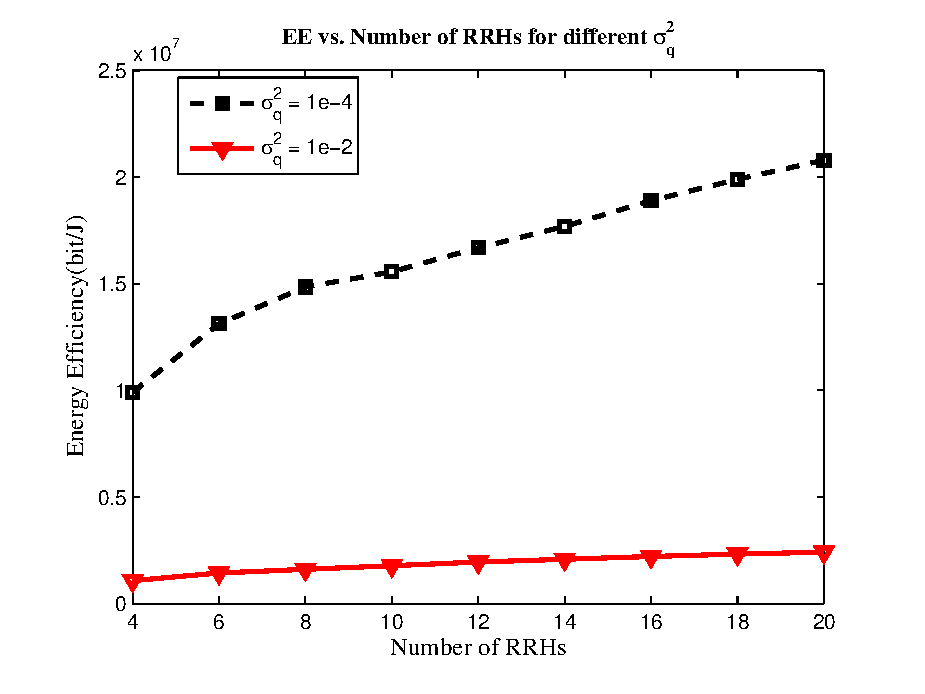
\includegraphics[width=\linewidth]{./fig/varq}
  \caption{ بازدهی انرژی برحسب تعداد واحد های رادیویی تک آنتنه برای واریانس های نویز کوانتیزاسیون متفاوت با فرض وجود 3 کاربر و $P_{max} = 23dBm$}
  \label{fig:varq}
  \end{figure}
 در شکل \ref{fig:varq} ، بازدهی انرژی بر حسب تعداد واحدهای رادیویی تک آنتنه با فرض وجود 3 کاربر و محدودیت 
لینک \lr{fronthaul}، $C_{max} = 5 (bit/s/Hz)$ برای دو نویز کوانتیزاسیون مختلف برای مدل سیستم اول رسم شده است. همانگونه که دیده می شود با افزایش نویز کوانتیزاسیون، بازدهی انرژی برای واحدهای رادیویی مختلف کاهش یافته است و با افزایش واحدهای رادیویی، بازدهی انرژی زیاد می گردد.
\begin{figure}[H]
  \centering
    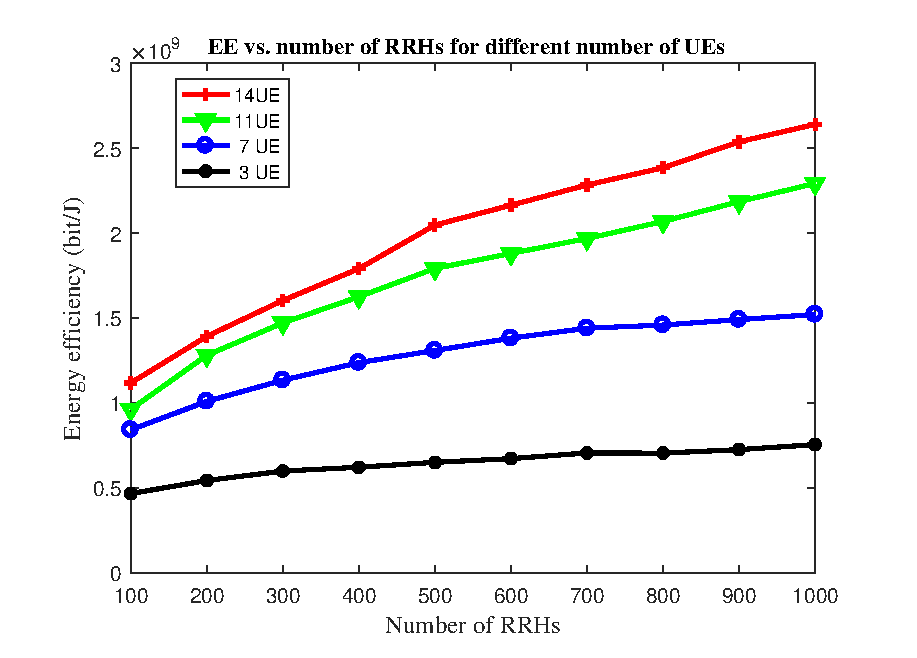
\includegraphics[width=\linewidth]{./fig/eeRRH}
  \caption{ .بازدهی انرژی برحسب تعداد واحدهای رادیویی برای یک خوشه برای تعداد کاربر متفاوت}
  \label{fig:eeRRH2}
  \end{figure}
حال برای مدل سیستم دوم شبیه سازی هایی ارائه می گردد.
%\begin{figure}[H]
%  \centering
%    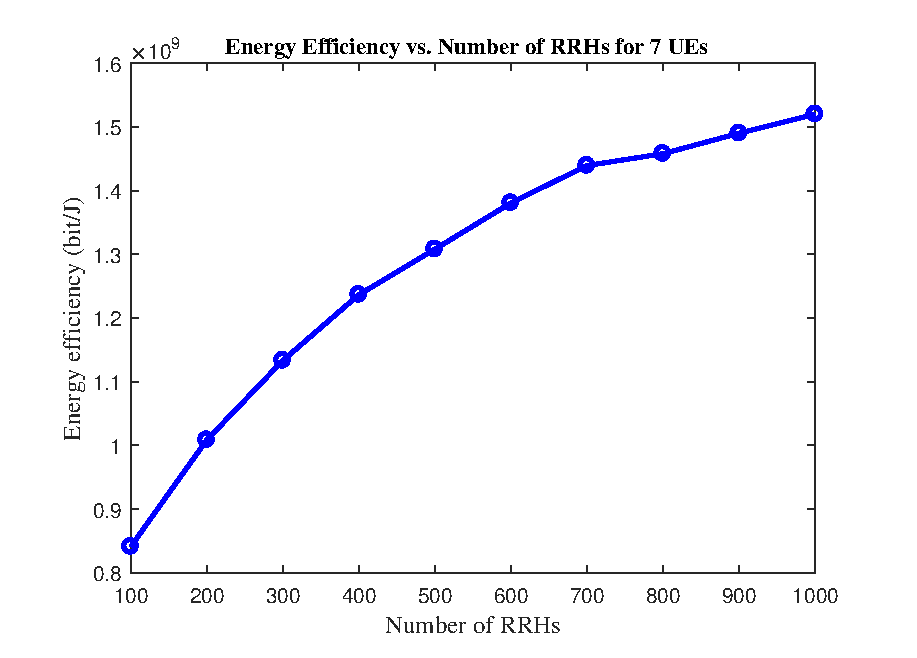
\includegraphics[width=\linewidth]{./fig/UE7}
%  \caption{ٍ بازدهی انرژی برحسب تعداد واحدهای رادیویی برای یک خوشه برای 7 کاربر }
%  \label{fig:UE7}
%  \end{figure}
در مدل سیستم دوم با فرض اینکه در ابتدا خوشه بندی صورت نگرفته باشد، با استفاده از روش الگوریتم تکرار شونده، بازدهی انرژی را برحسب تعداد واحدهای رادیویی برای یک خوشه با تعداد کاربران متفاوت  در شکل \eqref{fig:eeRRH2} با فرض استفاده از پیش کدگذاری \lr{MRT} رسم شده است. در این شکل فرض این است که ظرفیت محدود لینک \lr{fronthaul} و همچنین خوشه بندی در نظر گرفته نشده است. همانطور که در شکل \eqref{fig:eeRRH2} می بینید با افزایش تعداد واحدهای رادیویی، بازدهی انرژی بهبود می یابد. \newline
همچنین برای  شرایط گفته شده، در شکل \eqref{fig:eeUE}، بازدهی انرژی برحسب تعداد کاربران برای دو سری واحدهای رادیویی مختلف کشیده شده است.
\begin{figure}[H]
  \centering
    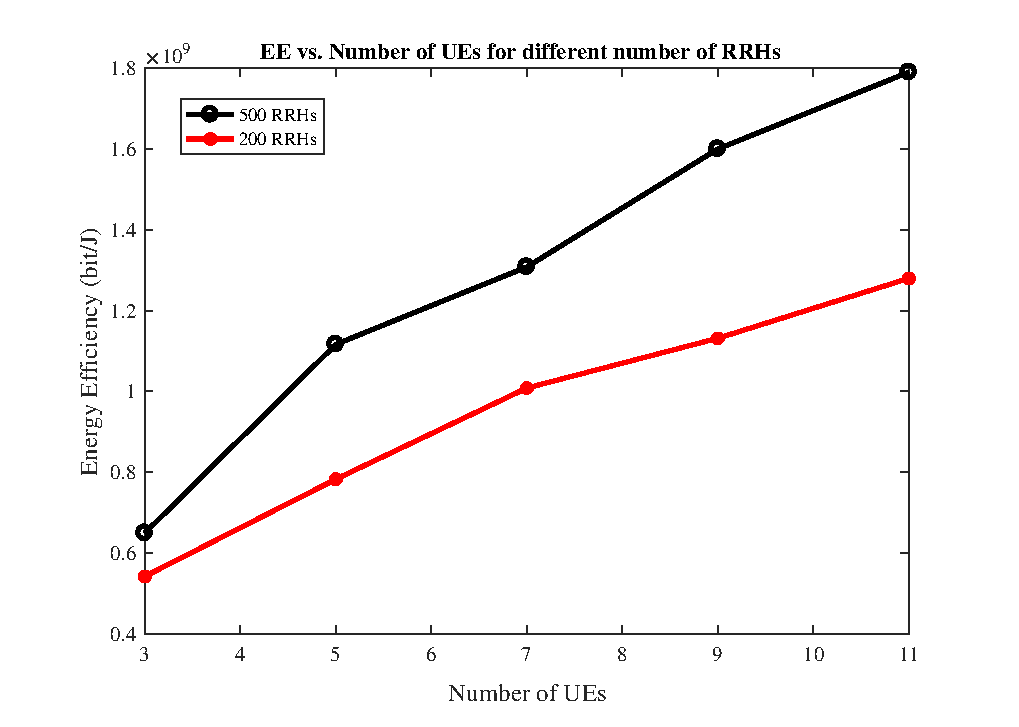
\includegraphics[width=\linewidth]{./fig/eeUE}
  \caption{ٍ بازدهی انرژی برحسب تعداد واحدهای رادیویی برای یک خوشه برای تعداد کاربر متفاوت}
  \label{fig:eeUE}
  \end{figure}
  حال میزان بازدهی انرژی برحسب تعداد واحدهای رادیویی برای دو نوع پیش کدگذاری \lr{MRT} و \lr{MMSE}  برای 3 کاربر در شکل ، نمایش داده شده است.
  با توجه به شکل، پیش کدگذاری \lr{MMSE}، منجر به بازدهی انرژی بیشتری می گردد زیرا با افزایش کاربران تداخل بیشتر شده و پیش کدگذاری \lr{MMSE} در حذف تداخل بهتر از \lr{MRT} عمل می کند.
  
\begin{figure}[H]
  \centering
    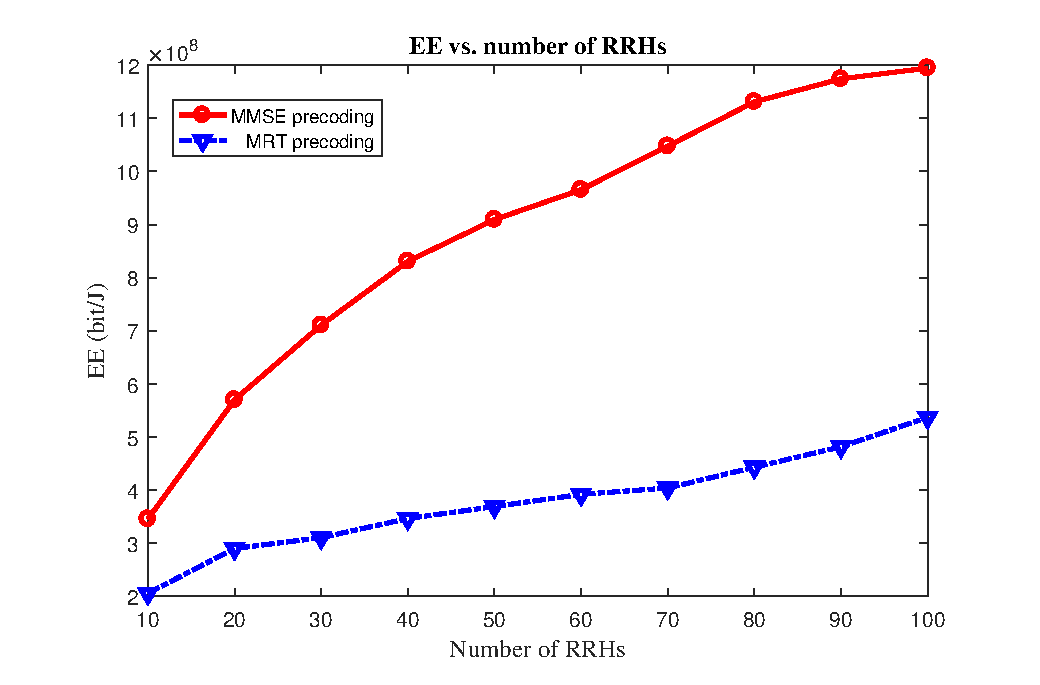
\includegraphics[width=\linewidth]{./fig/precode}
  \caption{
  بازدهی انرژی برحسب تعداد واحدهای رادیویی برای 3 کاربر در دو حالت با پیش کدگذاری متفاوت. }
  \label{fig:precode}
  \end{figure}
  همچنین در شکل \ref{fig:clus}، با فرض وجود 3 خوشه و 3 کاربر در هر خوشه بازدهی انرژی بر حسب تعداد واحدهای رادویی در هر خوشه رسم شده است که در شکل با افزایش تعدا واحدهای رادیویی در هر خوشه بازدهی افزایش می یابد.
  \begin{figure}[H]
  \centering
    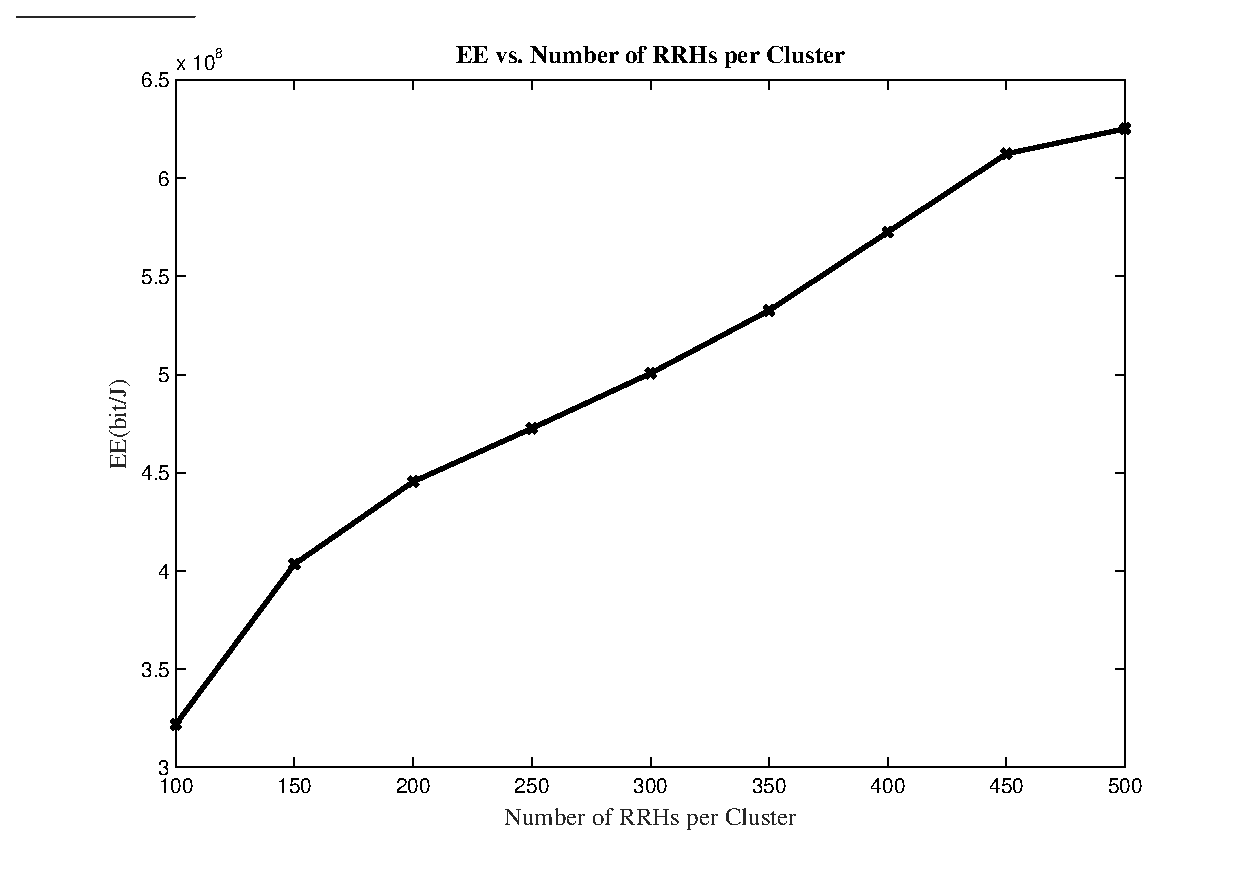
\includegraphics[width=\linewidth]{./fig/f2}
  \caption{
  بازدهی انرژی بر حسب تعداد واحدهای رادیویی با وجود 3 خوشه. }
  \label{fig:clus}
  \end{figure}
\section{لینک فراسو}
در این قسمت کارهای انجام شده در زمینه ی سیستمهای  \lr{MIMO C-RAN}  را در حالت فراسو مورد بررسی قرار گرفته است. در حالت فراسو، پیام از کاربران به واحد رادیویی ارسال می گردد و از طریق لینک \lr{fronthaul} که فیبر نوری است به واحد کنترل برای پردازش انتقال می یابد.
\subsection{مدل سیستم اول}
هدف از این بخش، بررسی لینک فراسو برای مدل سیستم خاص می باشد\cite{ul_dl,ulSimeone, Fronthaul, precodSimeone}. که در شکل \eqref{fig:ul2}، مسیر انتقال پیام از واحد رادیویی به واحد کنترل نمایش داده شده است.
فرض بر این است که در این حالت، سیستم شامل $N_U$ تا کاربر و $N_R$ 
تا واحد رادیویی است. 

\begin{figure}[H]
  \centering
    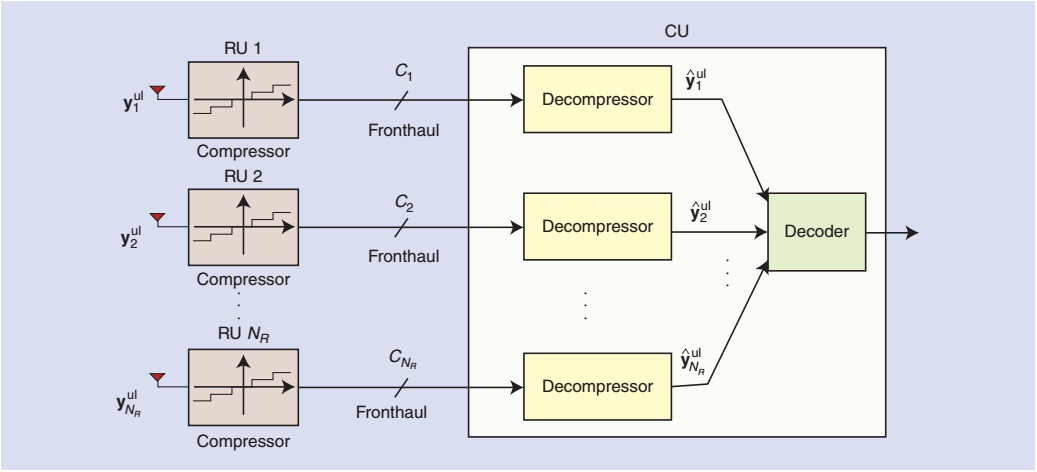
\includegraphics[width=\linewidth, height=6cm]{ul2}
  \caption{مسیر انتقال پیام در لینک فراسو \cite{Fronthaul}.}
  \label{fig:ul2}
\end{figure}
در اینجا همانند لینک فروسو، ساختار سیستم به صورت \lr{MIMO C-RAN} می باشد.  همچنین فرض می کنیم که هر واحد رادیویی دارای $N_r$ تا آنتن و هر کاربر تک آنتنه می باشد.\newline
در این مدل سیستم  زمان ارسال پیام به دو بخش تقسیم می گردد. بخشی از زمان در ابتدا برای ارسال پایلوت و بخشی دیگر صرف ارسال پیام می گردد. کل زمان ارسال پیام را $T$ در نظر گرفته  که به دو بخش $T_p$ برای ارسال پایلوت و یادگیری کانال و $T_d$ برای ارسال داده می باشد:
\begin{equation}
T = T_p + T_d
\end{equation}
سیگنال ارسالی توسط هر کاربر دارای ابعاد $1 \times T$ می باشد.
سیگنال ارسالی توسط کاربر $i$ام با نماد $\boldsymbol{X}_i$نشان داده شده که دارای توان 
 $\frac{1}{T} \mathit{E}[||\boldsymbol{X}_{i} ||^2] = P_{i}$
است. این سیگنال
به دو قسمت تقسیم می شود. قسمت اول
 $X_{p,i}$
  برای ارسال پایلوت است و دارای توان 
 $\frac{1}{T_p} \mathit{E}[||\boldsymbol{X}_{p,i} ||^2] = P_{p,i}$
می باشد و قسمت دوم
 $X_{d,i}$
 برای ارسال داده است و دارای توان 
 $\frac{1}{T_d} \mathit{E}[||\boldsymbol{X}_{d,i} ||^2] = P_{d,i}$
 می باشد.
 همچنین این توانها در معادله ی داده شده صدق می کنند:
 \begin{equation}
 \frac{T_p}{T}P_{p,i} +  \frac{T_d}{T}P_{d,i} = P_i
 \end{equation}
به علاوه سیگنال  یادگیری کانال که همان پایلوت است به صورت
 $\boldsymbol{X}_p = [\boldsymbol{X}_{p,1}^T,...,\boldsymbol{X}_{p,N_U}^T]^T$
است و
  $\boldsymbol{X}_d = [\boldsymbol{X}_{d,1}^T,...,\boldsymbol{X}_{d,N_U}^T]^T$
  سیگنال داده است.
 علاوه بر این،  
 $\boldsymbol{X}_p = \sqrt{P_p} \boldsymbol{S}_p$
 و 
  $\boldsymbol{X}_d = \sqrt{P_d} \boldsymbol{S}_d$
  که در اینجا $\boldsymbol{S}_p$ و $\boldsymbol{S}_d$ به ترتیب بردارهای $N_U \times T$ هستند 
  که نرمالیزه شده اند.
  
  
  پیام دریافتی توسط  $j$ امین واحد رادیویی برای دو حالت پیام یادگیری کانال و داده در ادامه بیان شده است:
  \begin{equation}\label{ypd}
  \begin{split}
 \boldsymbol{Y}_{p,j} &= \sqrt{P_p} \boldsymbol{H}_j \boldsymbol{S}_p + \boldsymbol{Z}_{p,j}\\
  \boldsymbol{Y}_{d,j} &= \sqrt{P_d} \boldsymbol{H}_j \boldsymbol{S}_d + \boldsymbol{Z}_{d,j}\\
 \end{split}
  \end{equation}
  در معادله ی \eqref{ypd}، $\boldsymbol{Z}_{p,j}$ و $\boldsymbol{Z}_{d,j}$ نویز گوسی جمع شونده
   $\boldsymbol{Z} \backsim \mathcal{N}(0,1)$ 
   می باشند و بردارهای آنها به ترتیب دارای $N_r \times T_p$ و
   $ N_r \times T_d$
     ابعاد است. همچنین بردار$\boldsymbol{H}_j $ ،نشان دهنده ی بردار کانال از کاربران به  $j$ امین واحد رادیویی می باشد که می توان به صورت $\boldsymbol{H}_j = [\boldsymbol{h}_{j,1},..., \boldsymbol{h}_{j,N_U}]$ بسط داد و دارای ابعاد  $N_r \times N_u$ می باشد.
    بردار کانال  
    $\boldsymbol{h}_{j,1}$
     در اینجا به صورت 
     $iid \backsim \mathcal{N}(0,\alpha_{j,i})$
       مدل شده است که 
      $\alpha_{j,i} = \frac{1}{1 + \frac{d_{ji}}{d_0}}$
      می باشد.
      
      حال، همانطور که در شکل \eqref{fig:ul2} ، دیده می شود، پیام دریافتی توسط واحد رادیویی، فشرده سازی می گردد \cite{uljmimo} که در اینجا برای دو بخش پایلوت و داده جداگانه بررسی می کنیم.
      \subsubsection{ مرحله ی یادگیری کانال   }
    در طول این مرحله، فشرده سازی و کوانتیزاسیون برای سیگنال   
    $ \boldsymbol{Y}_{p}$
    اعمال می گردد و می توان به حالت زیر نوشت
    
      \begin{equation}\label{yp}
      \hat{\boldsymbol{Y}}_{p} = \boldsymbol{Y}_{p} + \boldsymbol{Q}_{p}
      \end{equation}
      در معادله ی \eqref{yp}، 
       $\boldsymbol{Q}_{p} \backsim \mathcal{N}(0,\sigma_{p}^2 \boldsymbol{I} )$ 
         و \lr{iid}
       
         می باشد که
      $\sigma_{p}^2$
      تابع محدودیت لینک   
      \lr{fronthaul}
      می باشد.
       \newline
       حال با توجه به معادله ی  \eqref{yp}
       کانال بین کاربران و واحدهای رادیویی بوسیله ی \lr{MMSE} با خطا تخمین زده می شوند.
       \begin{equation}
       \boldsymbol{H} = \hat{\boldsymbol{H}} + \boldsymbol{E}
       \end{equation}
       که کانال تخمین زده ی $\hat{\boldsymbol{H}}$، ماتریس گوسی به صورت
        $\hat{\boldsymbol{H}} :iid \backsim \mathcal{N}(0,\sigma_{\hat{h}}^2)$ 
         و  $\hat{\boldsymbol{E}}: iid \backsim \mathcal{N}(0,\sigma_{e}^2)$  می باشد.
        همچنین $\sigma_{\hat{h}}^2 =\alpha - \sigma_{e}^2$ است.
      
     
  \subsubsection{ مرحله ی بررسی داده  }
  در این مرحله، داده فشرده سازی و کوانتیزاسیون می گردد.
  
    \begin{equation}\label{yd}
      \hat{\boldsymbol{Y}}_{d} = \boldsymbol{Y}_{d} + \boldsymbol{Q}_{d}
      \end{equation}
      در معادله ی \eqref{yd}،  $\boldsymbol{Q}_{d} :iid \backsim \mathcal{N}(0,\sigma_{d}^2)$  می باشد.
علاوه بر این نویز معادل به صورت  $\boldsymbol{N}_{d}=\boldsymbol{E} \boldsymbol{X}_{d}+\boldsymbol{Z}_{d}+\boldsymbol{Q}_{d}$ تعریف می گردد.  
      همچنین داریم:
      
      
  \begin{equation}
  \hat{\boldsymbol{Y}}_{d} =  \hat{\boldsymbol{H}} \boldsymbol{X}_{d} + \boldsymbol{N}_{d}
  \end{equation}
  که در اینجا
    $\boldsymbol{N}_{d} :iid$
    با میانگین صفر و توان 
  $  1+\sigma_{d}^2 + P_d \sigma_{e}^2$
  است که نویز گوسی می باشد که مستقل از 
  $\boldsymbol{X}_{d} $
  نیست.
 \subsubsection{صورت مسئله}
 در ابتدای این بخش نرخ قابل دسترس و ظرفیت لینک محاسبه می گردد سپس  صورت مسئله بیان می شود.
 کران پایین برای نرخ قابل دسترس برای مدل سیستم بیان شده با توجه به مقالات به صورت زیر است:
 \begin{equation}
 R = \frac{T_d}{T} \mathcal{E}\{\log_2{det (\boldsymbol{I}_{N_r}+\rho_{eff} \hat{\boldsymbol{H}} \hat{\boldsymbol{H}}^{H} )}\}
 \end{equation}
 که در اینجا $\rho_{eff} = P_d / ( 1+\sigma_{d}^2 + P_d \sigma_{e}^2)$ می باشد.
 علاوه بر این در ادامه ظرفیت لینک \lr{frotnhaul} را بدست می آید. در اینجا فرض بر این است که  $C_p$ ظرفیت بخش پایلوت و $       C_d$   ظرفیت داده در این لینک باشد در نتیجه ظرفیت کل لینک برابر است با 
 $\bar{C} = C_p +C_d.$
که در اینجا
 \begin{equation}
 \begin{split}
 C_p & = \frac{Tp N_r}{T} \log_2 (1 + \frac{P_p \alpha +1}{\sigma_p^2})\\
  C_d & = \frac{Td N_r}{T} \log_2 (1 + \frac{P_d \alpha +1}{\sigma_d^2})
 \end{split}
 \end{equation}
 است.
 حال در این حالت، مجموع نرخ های قابل دسترس براساس محدودیت ظرفیت لینک \lr{fronthaul} و محدودیت توان هر واحد رادیویی، بیشینه می گردد:
\begin{equation}
\begin{aligned}
\max\limits_{P_d,P_p}   \quad &   \sum R(P_d)\\
\text{\lr{subject to}} \quad  & \bar{P}_i \leq P_{max} \ \  \forall i \\
&\bar{C} ({P_d,P_p})\leq C^{th} \\
\end{aligned}
\end{equation}
 \subsection{مدل سیستم دوم}
 در این قسمت مدل سیستم دیگری برای لینک فراسو در نظر گرفته شده است \cite{ofdma,ulCompression,dlulP}.
 در این مدل سیستم فرض بر این است که 
 $N$
 تا واحد رادیویی داریم که $K$ کاربر را سرویس دهی می کنند همچنین فرض بر این است که واحدهای رادیویی و کاربران تک آنتنه هستند. برخلاف مدل سیستم قبل، در این بخش یادگیری کانال و یا پایلوت در مدل سیستم بیان نمی شود و صرفا مرحله ی پردازش داده مورد بررسی قرار می گیرد. همچنین از خوشه بندی کاربران و واحدهای رادیویی صرف نظر می گردد.
 سیگنال دریافتی توسط $n$ امین واحد رادیویی که با $y_n$  نمایش می دهیم به وسیله ی معادله ی زیر بدست می آید:
 \begin{equation}
 y_n = \sum_{k=1}^{K} h_{n,k} \sqrt{p_k} s_k + z_n
 \end{equation}
 که در اینجا، $h_{n,k}$ مقدار کانال از $k$ امین کاربر به $n$ امین واحد رادیویی می باشد. علاوه بر این، $p_k$ توان ارسالی کاربر $k$ ام می باشد و $s_k$ پیام کاربر $k$ ام است. نیز $z_n$ نویز گوسی جمع شونده ی دریافتی برای $n$ امین واحد رادیویی است که دارای میانگین صفر و واریانس $\sigma_n^2$ می باشد.
 $z_n \backsim \mathcal{N}(0,\sigma_n^2)$ 

همچنین همانطور که قبلا گفته شده به دلیل محدودیت ظرفیت لینک \lr{fronthaul} پیام دریافتی توسط واحد رادیویی فشرده شده و سپس از طریق این لینک به واحد کنترل ارسال می گردد.
پیام فشرده شده به این صورت بیان می گردد.
\begin{equation}\label{yq}
\tilde{y}_n = y_n + q_n
\end{equation} 
که در اینجا
 $q_n \backsim \mathcal{N}(0,\sigma_q^2) \ \ \forall n$ 
 نویز گوسی جمع شونده می باشد.
 در نتیجه با توجه به رابطه ی \eqref{yq}، نرخ انتقال پیام از $n$ امین واحد رادیویی به واحد کنترل از طریق لینک \lr{fronthaul} به شرح زیر است.
 \begin{equation}
 C_n = B \log_2 (1+ \frac{\sum_{k=1}^{K} |h_{n,k}|^2 p_k}{\sigma_q^2})
 \end{equation}
 
پیام فشرده شده پس از انتقال به واحد کنترل از طریق لینک با ظرفیت محدود، در این واحد کنترل به صورت خطی ترکیب می گردد تا بتوان سیگنال هر پیام را تخمین زد.
در نتیجه برای بدست آوردن سیگنال $s_k$ که توسط کاربر ارسال شده است از روش تشخیص \lr{MRC} که همان ترکیب خطی بین پیامهای دریافتی است، استفاده می نماییم.
\begin{equation}\label{sk}
\hat{s}_k = \boldsymbol{w}_k^H \tilde{\boldsymbol{y}}
\end{equation}
در معادله ی بالا،
 $\boldsymbol{w}_k = [w_{1,k},...,w{N,k}]$
 
 همان بردار تشخیص است که $w_{i,k} = h_{i,k}^*$ می باشد.
همچنین در اینجا بردار $\tilde{\boldsymbol{y}}$ به حالت مقابل تعریف می شود، 
$\tilde{\boldsymbol{y}} = [ \tilde{y}_1,..., \tilde{y}_N]$
حال می توان معادله ی \eqref{sk} را به شکل زیر بسط داد.
\begin{equation}\label{skext}
\begin{split}
\hat{s}_k &= \underbrace{\boldsymbol{w}_k^H \boldsymbol{h}_k \sqrt{P}_k s_k }_{\text{(\lr{desired signal})}} \\
&+\underbrace{ \sum_{k=1,j \neq k}^{K}  \boldsymbol{w}_k^H \boldsymbol{h}_j \sqrt{P}_j s_j}_{\text{(\lr{interference signal})}}  \\
&+ \underbrace{\boldsymbol{w}_k^H (\boldsymbol{z}+\boldsymbol{q})}_{\text{(\lr{quantisation and additive noise})}}\\
\end{split}
\end{equation}
در معادله ی ذکر شده، $\boldsymbol{h}_k$ بردار کانال از کاربر $k$ ام به تمام واحدهای رادیویی است که می توان به صورت $\boldsymbol{h}_k = [h_{1,k},...,h_{N,k}]$ نوشت. به همین منوال،
 $\boldsymbol{z} = [z_{1},...,z_{N}]$
و نیز $
\boldsymbol{q} = [q_{1},...,q_{N}]$
می باشد.
\subsubsection{صورت مسئله}
همان طور که می دانیم نرخ قابل دسترس برای $k$ امین کاربر به این صورت بدست می آید.
\begin{equation}
R_k = B \log_2(1+ \gamma_k)
\end{equation}
که $ \gamma_k$ همان \lr{SINR} برای $k$ امین کاربر می باشد. با توجه به معادله ی \eqref{skext}، $\gamma_k$ از رابطه ی زیر بدست می آید
\begin{equation}
\gamma_k = \frac{p_k |\boldsymbol{w}_k^H \boldsymbol{h}_k|^2}{\sum_{k=1,j \neq k}^{K} p_j |\boldsymbol{w}_k^H \boldsymbol{h}_j|^2 + (\sigma_n^2+\sigma_q^2) ||\boldsymbol{w}_k||^2}
\end{equation}


 همانطور که گفته شد نسبت مجموع نرخ ها در سیستم به کل توان ارسالی کاربرها نشان دهنده ی بازدهی انرژی است که با $\eta$ نمایش داده می شود و می توان اینگونه بیان کرد
\begin{equation}\label{eta1}
\eta(\boldsymbol{P}) = \frac{\sum\limits_{k=1}^{K}{R}_{k} }{ \sum\limits_{k=1}^{K}{p}_{k}}= \frac{R_{total}(\boldsymbol{P})}{P_{UE}(\boldsymbol{P})},
\end{equation}
حال در این مسئله، هدف بیشینه سازی بازدهی انرژی با شروط زیر می باشد:
 \begin{equation}\label{p11}
\begin{aligned}
\max\limits_{\boldsymbol{P}}   \quad &   \eta(\boldsymbol{P})\\
\text{\lr{subject to}} \quad  &  0 \leq {p}_{k} \leq P_{max} && \qquad \forall k,   \\
&{R}_{k} \geq {R}_{k}^{th} && \qquad \forall k, \\ 
&C_{n} \leq C_{n}^{th}  &&\qquad  \forall i, \\
\end{aligned}			
\end{equation}
برای بدست آوردن توان بهینه، از تابع لاگرانژ و الگوریتم تکرار شونده استفاده می شود که در فصل 3 به طور کامل شرح داده می شود.
  \subsection{نتایج عددی}
  در این بخش، نتایج عددی الگوریتم مورد استفاده را برای سیستم  با پرتو دهی \lr{MRT} و با پارامترهای بیان شده در جدول \ref{tab:title3} \cite{ofdma} بیان می شود.
\begin{latin} 
 \begin{table}[H]
 \caption {\rl{پارامترهای شبیه سازی}} \label{tab:title3} 
 \begin{center}
  \begin{tabular}{||c c ||} 
  \hline
  Parameter & Value \\ [0.5ex] 
  \hline\hline
  Number of cluster S & 1 \\ 
  \hline
    The radius of the cell & 500m \\ 
  \hline
  Noise power density & -174dBm/Hz\\
  \hline
  Bandwidth & 1MHz \\
  \hline
 Maxmimun transmit Power & 23dBm \\
  \hline
Circuit Power of whole RRHs & 10dBm \\
  \hline
  Minimum data rate &  0.1bits/sec/Hz \\ [1ex] 
  \hline
 \end{tabular}
 \end{center}
 \end{table}
 \end{latin}

\begin{figure}[H]
  \centering
    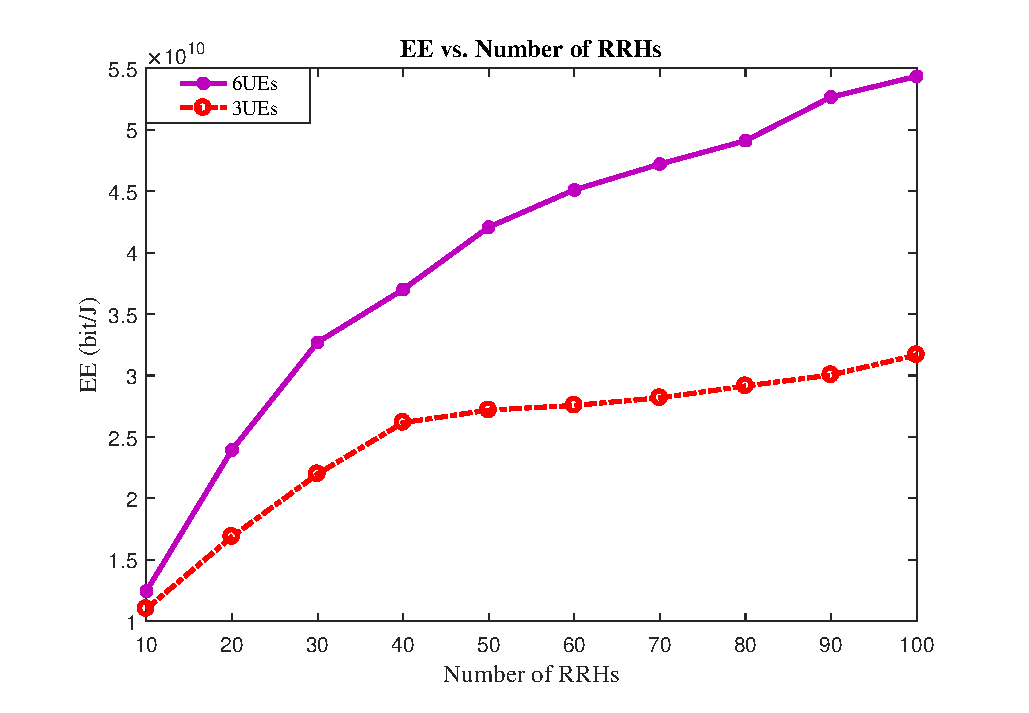
\includegraphics[width=\linewidth]{./fig/rrhul}
  \caption{ٍ بازدهی انرژی برحسب تعداد واحدهای رادیویی برای یک خوشه برای 2 کاربر متفاوت}
  \label{fig:rrhul}
  \end{figure}
 حال بازدهی انرژی را برحسب تعداد واحدهای رادیویی برای یک خوشه با تعداد کاربران متفاوت  در شکل \eqref{fig:eeRRH2} با فرض استفاده از پیش کدگذاری \lr{MRT} رسم شده است. در این شکل فرض این است که ظرفیت محدود لینک \lr{fronthaul} و همچنین خوشه بندی در نظر گرفته نشده است. همانطور که در شکل می بینید با افزایش تعداد واحدهای رادیویی، بازدهی انرژی بهبود می یابد.

\begin{figure}[H]
  \centering
    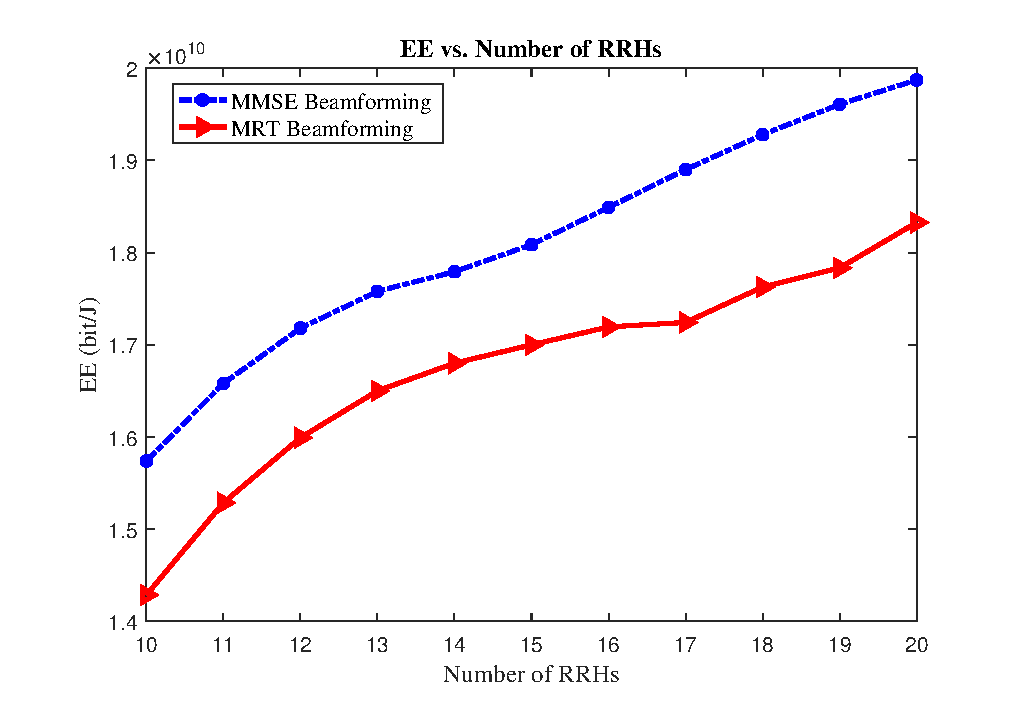
\includegraphics[width=\linewidth]{./fig/beamforming}
  \caption{ٍ بازدهی انرژی برحسب تعداد واحدهای رادیویی برای2 کاربر  در دو حالت با پرتودهی متفاوت }
  \label{fig:beam}
  \end{figure}
      حال میزان بازدهی انرژی برحسب تعداد واحدهای رادیویی برای دو نوع پیش کدگذاری \lr{MRT} و \lr{MMSE}  برای 2 کاربربا فرض های گفته شده برای شکل قبلی،  در شکل \ref{fig:beam} ، رسم کرده ایم.
  با توجه به شکل ، می توان فهمید که پیش کدگذاری \lr{MMSE}، منجر به بازدهی انرژی بیشتری می گردد زیرا \lr{MRT} اثر بیشتری در حذف نویز داشته در صورتی که \lr{MMSE} تداخل را بهتر از بین می برد و در اینجا تاثیر نویز از تداخل کمتر است .


 \begin{figure}[H]
  \centering
    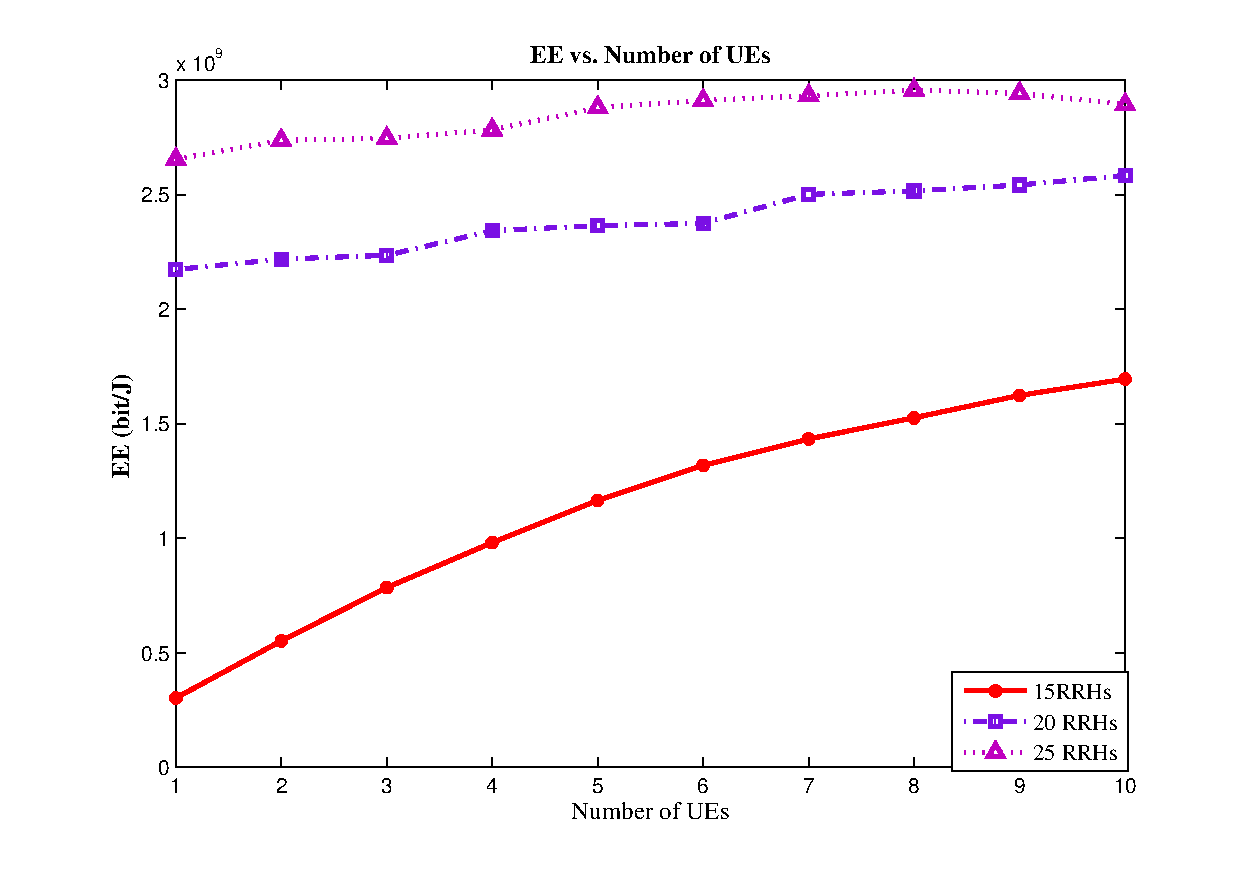
\includegraphics[width=\linewidth]{./fig/ue1}
  \caption{ٍ بازدهی انرژی برحسب تعداد کاربران برای یک خوشه برای
   3
   مقدار متفاوت واحد های رادیویی}
  \label{fig:ue1}
  \end{figure}
  در شکل \ref{fig:ue1}، بازدهی انرژی برحسب تعداد کاربران برای یک خوشه برای 3 مقدار متفاوت واحد های رادیویی با فرض $P_{max} = 10dbm$ رسم شده است. در این نمودار بیشینه ی ظرفیت محدود لینک \lr{fronthaul} مقدار 5 در نظر گرفته شده است و واریانس نویز کوانتیزاسیون $10^{-8}$ می باشد. با افزایش کاربران، بازدهی انرژی زیاد می گردد و  از جایی به بعد شیب افزایش آن رو به کاهش است که این کاهش به دلیل تداخل کاربران می باشد.
 
\begin{figure}[H]
  \centering
    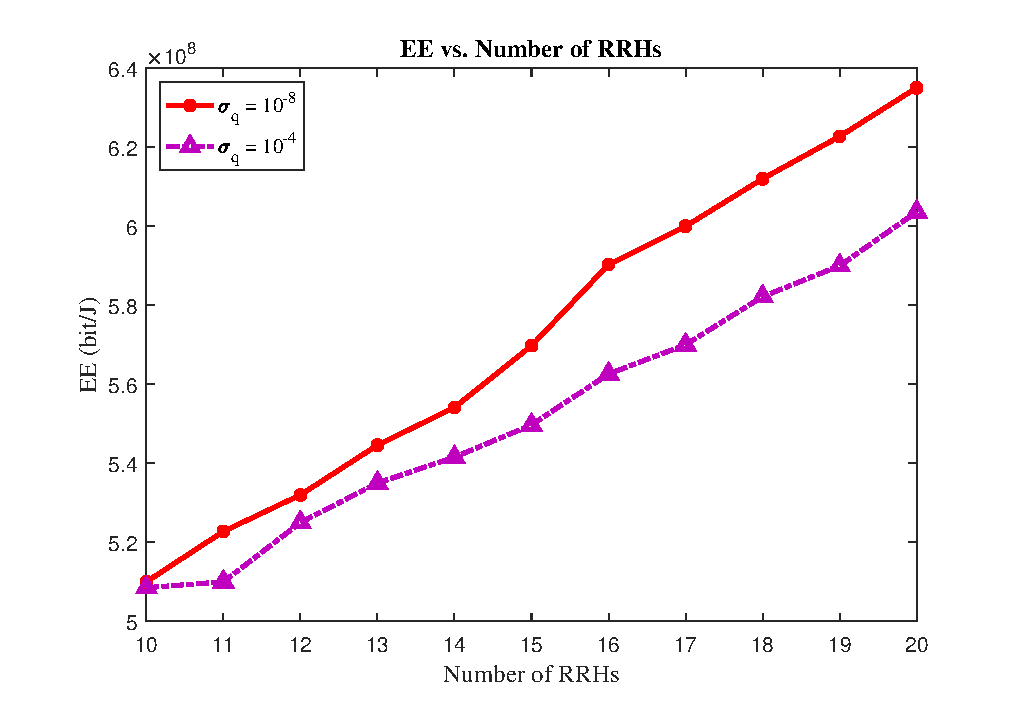
\includegraphics[width=\linewidth]{./fig/sigmaul}
  \caption{ٍ بازدهی انرژی برحسب تعداد واحدهای رادیویی برای2 کاربر  در دو حالت با نویز کوانتیزاسیون متفاوت }
  \label{fig:sigmaul}
  \end{figure}
      حال میزان بازدهی انرژی برحسب تعداد واحدهای رادیویی  در دو حالت با نویز کوانتیزاسیون متفاوت برای 2 کاربربا فرض های گفته شده برای شکل قبلی،  در شکل \ref{fig:sigmaul} ، رسم شده است.
  با توجه به شکل ، می توان فهمید که بازدهی انرژی برای زمانی که میزان نویز کمتر است بیشتر می باشد.
\subsection{مقایسه ی روش های بیان شده}
در این بخش، مدل سیستمهای مختلف در لینک فراسو با یکدیگر مقایسه می شوند.
درهردو مدل سیستم فشرده سازی و محدودیت لینک \lr{fronthaul} مورد بررسی قرار گرفته شده است. همچنین در هر دو فرض شده که خوشه بندی صورت نگرفته است. 

در مدل سیستم اول، سیگنال یادگیری کانال نیز در ابتدا ارسال می گردد تا بتوان کانال را تخمین زد. ولی در مدل سیستم دوم فرض بر این است که تخمین کانال از قبل صورت گرفته شده است و در مورد تخمین کانال صحبتی صورت نمی گیرد. همچنین در مدل سیستم دوم از ترکیب خطی 
\lr{MRC}\LTRfootnote{Maximum Ratio Combination}
برای بازیابی سیگنال استفاده می گردد که در مدل سیستم اول مورد بررسی قرار نمی گیرد.
در مدل سیستم اول، هدف ما، بیشینه سازی مجموع نرخهای قابل دسترس است در صورتی که در مدل سیستم دوم هدف بیشینه سازی بازدهی انرژی می باشد.

\section{سیستم مخابراتی \lr{D2D} }
\subsection{مقدمه}
در این بخش مدل سیستم دیگری بیان می شود که دارای سیستم مخابراتی \lr{D2D} 
\LTRfootnote{Device-to-Device}
 می باشد \cite{d2d, d2dd} . سیستم \lr{D2D} منجر می شود که ساختار \lr{C-RAN} بازدهی طیفی بیشتر و تاخیر کمتری داشته باشد. در حال حاضر، تحقیقات زیادی در زمینه ی تخصیص منابع برای سیستم های مخابراتی \lr{D2D} صورت گرفته است.
 حال در اینجا این مدل سیستم در ساختار \lr{C-RAN} بررسی می شود \cite{rd2d}.
 \subsection{مدل سیستم}
  در این ساختار، شبکه دارای $N$ تا واحد رادیویی یا \lr{RRH} $M$ آنتنه می باشد. همچنین این ساختار دارای $K$ جفت کاربر \lr{D2D} تک آنتنه می باشد که در هر جفت یکی فرستنده است که با $T_x$ نمایش داده می شود و دیگری گیرنده می باشد که با $R_x$ نمایش می دهیم. 
علاوه بر این فرض می شود واحد کنترل یا \lr{BBU pool} به خوبی می تواند کانال را تخمین بزند. 
همچنین این مدل سیستم در دو وضعیت \lr{C-RAN} و \lr{D2D} کار می کند که در بازه های زمانی مختلف در وضعیت های مختلف عمل می کند. 
فرض کنید در بازه ی زمانی  
$[t,t+1)$
سیگنال ارسالی از $k$ امین کاربر فرستنده ی  
$T_x$
، در وضعیت \lr{C-RAN} به صورت مقابل می باشد
\begin{equation}
\begin{split}
y^C_k(t) =& \sum_{n=1}^{N} \boldsymbol{v}_{n,k}^{H}(t) \boldsymbol{g}_{n,k}^{C}(t) \sqrt{p_k(t)} s_k(t) \\
+& \sum_{n=1}^{N} \sum_{l\neq k}^{K} \boldsymbol{v}_{n,k}^{H}(t) \boldsymbol{g}_{n,l}^{C}(t) \sqrt{p_l(t)} s_l(t) \\
+& \sum_{n=1}^{N} \boldsymbol{v}_{n,k}^{H}(t) \boldsymbol{z}_n(t)
\end{split}
\end{equation}
 که در اینجا، $\boldsymbol{v}_{n,k} \in \mathsf{C}^{M\times 1}$
  نشان دهنده ی بردار پرتو دهی بین
 کاربر $k$ ام  و  واحد رادیویی $n$ ام می باشد.

می باشد. 
 همچنین 
 $\boldsymbol{g}_{n,k}^{C}(t) \in \mathsf{C}^{M\times 1}$
 بردار کانال بین  کاربر $k$ ام  و  واحد رادیویی $n$ ام است.  
 $\boldsymbol{z}_n(t) \backsim \mathcal{N}(0,\sigma^2 \boldsymbol{I}_M )$
 نیز، بردار نویز گوسی است.
علاوه بر این، $p_k(t)$ و $s_k(t)$ به ترتیب نشان دهنده ی توان ارسالی و سیگنال ارسالی از کاربر $k$  می باشد. 
 در این وضعیت، نرخ قابل دسترس از رابطه ی زیر بدست می آید:
\begin{equation}
R^{C}_k(t) = \log_2(1+ \frac{p_k(t) |\boldsymbol{v}_{k}^{H}(t) \boldsymbol{g}_{k}^{C}(t)|^2 }{ \sum_{l\neq k}^{K}p_l(t) |\boldsymbol{v}_{k}^{H}(t) \boldsymbol{g}_{l}^{C}(t)|^2 + \sigma^2 || \boldsymbol{v}_{k}||^2_2})
\end{equation}
که در اینجا،$\boldsymbol{v}_{k} \in \mathsf{C}^{NM\times 1}$ بردار پرتودهی برای کاربر $k$ می باشد
که به صورت \\
 $\boldsymbol{v}_{k}^{C}(t) = [{\boldsymbol{v}_{1,k}^{C}(t)}^T, ... , {\boldsymbol{v}_{N,k}^{C}(t)}^T ]^T$
است. 
 همچنین 
 $\boldsymbol{g}_{k}^{C}(t) \in \mathsf{C}^{NM \times 1}$
 بردار کانال بین کاربر $k$ام و واحدهای رادیویی است.\newline
  که به صورت 
  $\boldsymbol{g}_{k}^{C}(t) = [{\boldsymbol{g}_{1,k}^{C}(t)}^T, ... , {\boldsymbol{g}_{N,k}^{C}(t)}^T ]^T$
 می باشد.
 به صورت مشابه، سیگنال دریافتی توسط کاربر $R_x$ در حالت \lr{D2D} به صورت مقابل می باشد:

\begin{equation}
y^D_i(t) =  {g}_{i,i}^{D}(t) \sqrt{p_i(t)} s_i(t) 
+ \sum_{j\neq i}^{K} {g}_{j,i}^{D}(t) \sqrt{p_j(t)} s_j(t) + \phi_i(t) 
\end{equation}
که در اینجا  
$ \boldsymbol{g}_{i,i}^{D}$
بردار کانال بین $i$ امین جفت فرستنده و گیرنده ی \lr{D2D} می باشند. همچنین 
 $\phi_i(t) \backsim \mathcal{N}(0,\sigma^2 )$
 نویز گوسی است.\newline
 نرخ قابل دسترس 
 در اینجا از رابطه ی زیر بدست می آید:
 \begin{equation}
R^{D}_k(t) = \log_{2} (1+ \frac{p_i(t) |g_{i,i}^{D}(t)|^2 }{ \sum_{j\neq i}^{K} p_j(t) |g_{j,i}^D (t)|^2 + \sigma^2 })
\end{equation}
برای انتخاب وضعیت های متفاوت در بازه ی زمانی $t$  برای جفت کاربر$k$ از رابطه ی زیر استفاده می شود.
%\begin{equation}
\begin{latin}
\[ 
x_k(t) =
\left \{
 \begin{tabular}{cc}
  0,  & \text{\lr{C-RAN mode}} \\
  1,  & \text{\lr{D2D mode}} \\
  \end{tabular}
  \right \}
\]
%\end{equation}
\end{latin}
بنابراین با توجه به  رابطه ی بالا نرخ قابل دسترس  برای  $k$ امین جفت کاربر به صورت زیر بدست می آید:
\begin{equation}
R_k(t)  = (1-x_k(t)) R_k^C(t) + x_k(t) R_k^D(t)
\end{equation}
میانگین نرخ قابل دسترس برای $k$ امین جفت \lr{D2D} از رابطه ی مقابل بدست می آید:
\begin{equation}
\bar{R_k} = \lim_{T\to\infty} \frac{1}{T} \sum_{t=0}^{T-1} \mathrm{E}\{R_k(t)\} 
\end{equation}
حال در اینجا هدف، بیشینه سازی مجموع میانگین نرخ قابل دسترس با شروطی که بیان می گردد، می باشد که در ادامه نمایش داده شده است.
   \begin{equation}
\begin{aligned}
\max\limits_{\boldsymbol{p}(t),  \boldsymbol{x}(t)}   \quad &   \sum_{k=1}^{K}(\bar{R_k})\\
\text{\lr{subject to}} \quad  &  0 \leq {p}_{k} \leq P_{max} && \qquad \forall k,   \\
& \sum_{k=1}^{K} x_k(t) p_k(t) \ P_{max}^{k} && \qquad \forall k, \\ 
&x_k(t) \in \{ 0, 1 \}  &&\qquad  \forall ik\\
\end{aligned}			
\end{equation}
\section{نتیجه گیری}
در این فصل ابتدا لینک فروسو و سپس لینک فراسو را مورد بررسی قرارگرفته است. در لینک فروسو سه مدل سیستم متفاوت بررسی شده اند که در فصل بعدی دو مدل سیستم اول را با یکدیگر ادغام کرده و مدل سیستم جدیدی بیان می شود. همچنین در لینک فراسو نیز دو مدل سیستم متفادت بیان شده است که در ادامه ی فصل سوم مدل سیستمی شامل چندین خوشه به همراه لینک محدود \lr{fronthaul} تعریف می شود. در قسمت آخر این فصل، مدل سیستم \lr{D2D} معرفی شده که در حال حاضر می توان در این زمینه، کارهای نوینی انجام داد. 

\chapter{تخصیص منابع در شبکه های دسترسی رادیویی ابری دارای ظرفیت محدود در لینک \lr{fronthaul}}
%\thispagestyle{empty}
\section{مقدمه}
در این فصل، هدف تخصیص منابع در شبکه های  دسترسی رادیویی ابری است که برای دو حالت لینک فراسو و لینک فروسو در نظر گرفته شده است. در اینجا فرض بر این است که واحدهای رادیویی، به صورت توزیع شده و مشارکتی همانند \lr{MIMO}، پیام را دریافت و یا ارسال می کنند که شبکه های دسترسی رادیویی ابری با مشارکت توزیع شده را ایجاد می نمایند.
برای استفاده از مزایای سیستمهای \lr{C-RAN} و \lr{MIMO}، از سیستم \lr{MIMO C-RAN} به طور همزمان استفاده می گردد که منجر به بهبود نرخ و بازدهی انرژی \lr{EE} می گردد. با استفاده از سیستم های \lr{MIMO}، می توان به نرخ داده ی بیشتری رسید.\newline
برای در نظر گرفتن لینک عملی بین واحد کنترل و واحد رادیوییها، که \lr{Fronthaul} نامیده می شود، ظرفیت لینک \lr{Fronthaul} محدود در نظر گرفته می شود. بنابراین، سیگنالی که از لینک \lr{Fronthaul} عبور می کند نیاز به فشرده سازی دارد.

در ادامه مدل سیستم برای لینک فروسو و فراسو بیان می شود.
\begin{figure}
  \centering
    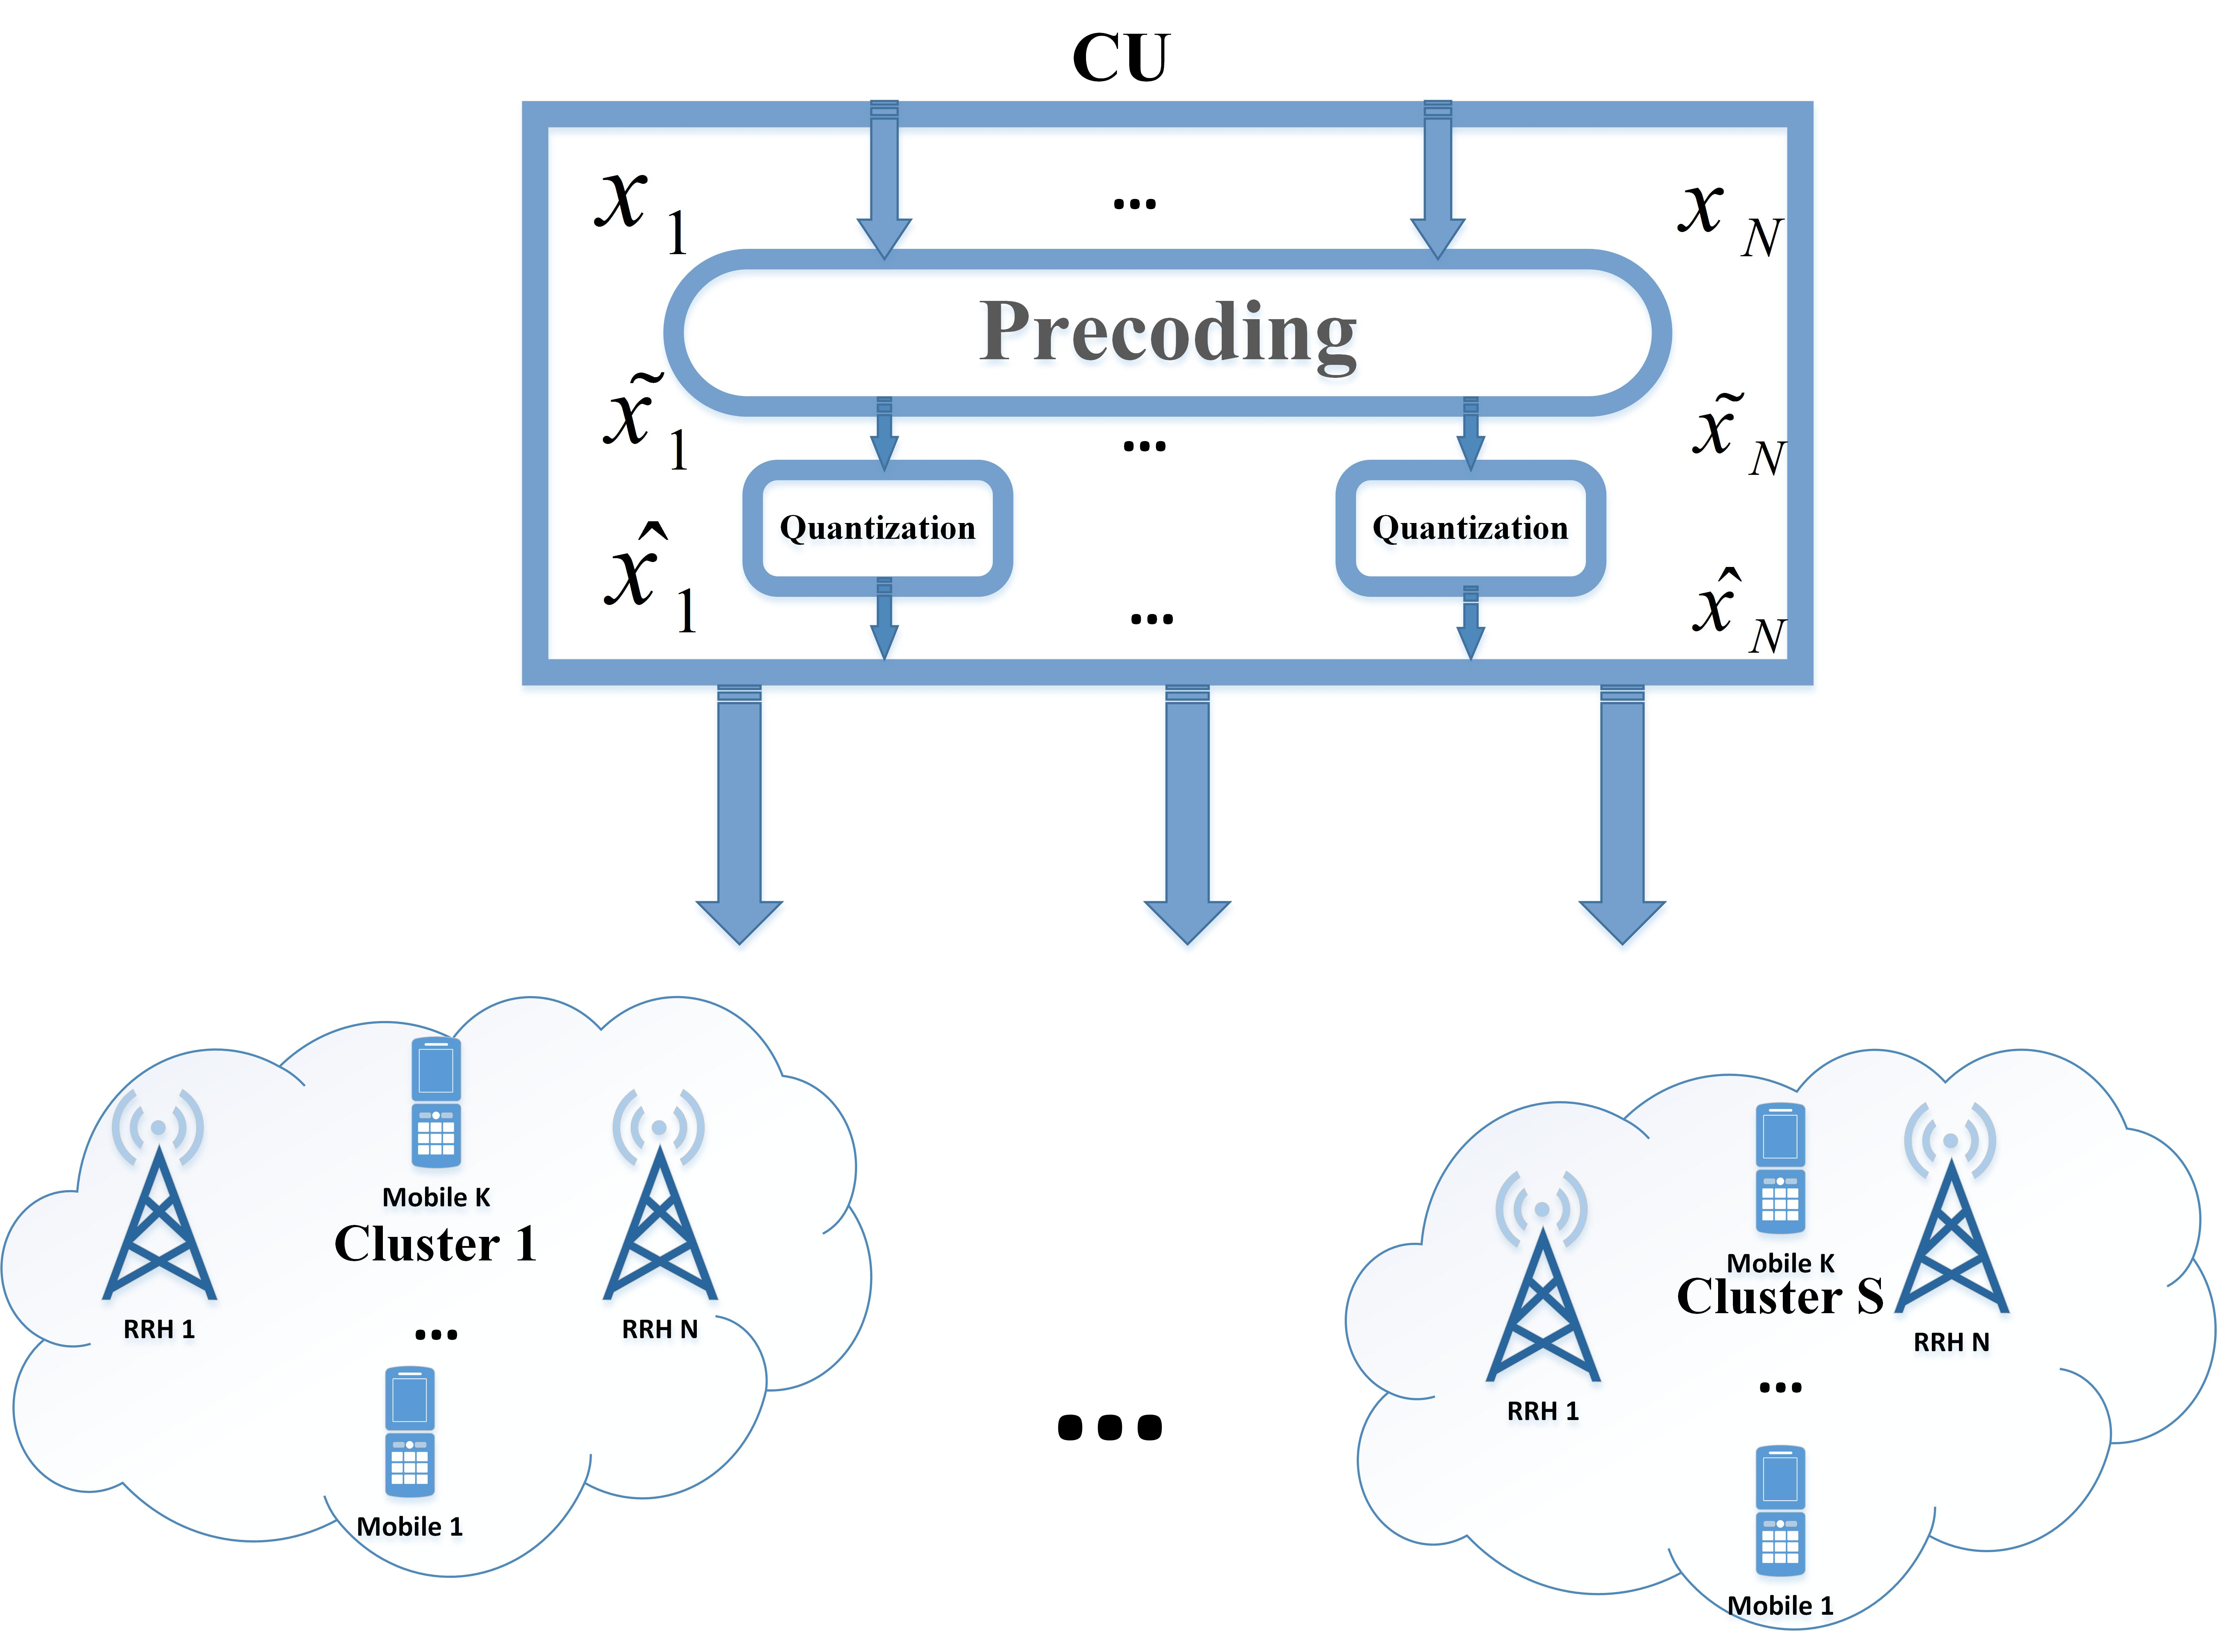
\includegraphics[width=\linewidth]{./fig/mydraw1}
  \caption{ساختار 
  \lr{C-RAN}
  در  لینک فروسو.
  }
  \label{fig:cr1}
\end{figure}
 فرض مسئله بر این است که سیستم به صورت چند آنتنه (\lr{MIMO})  می باشد و ظرفیت \lr{Fronthaul} محدود است. همچنین، سیستم دارای چندین خوشه یا سلول که در هر خوشه، تعدادی  واحد رادیویی و تعدادی کاربر قرار دارد\cite{EEcluster,jcluster}. هدف، بدست آوردن بیشینه بازدهی انرژی می باشد.\newline
 در حالت لینک فروسو، پیام، پیش کدگذاری شده است و سپس فشرده سازی بر روی آن صورت گرفته است و از طریق لینک \lr{Fronthaul} به واحد رادیویی منتقل می شود تا پیام را به کاربران ارسال کنند \cite{Fronthaul, ulSimeone, precodSimeone}
 .\newline
 در حالت لینک فراسو، سیگنال از کاربران به واحدهای رادیویی منتقل شده و سپس پیام فشرده شده و به دست واحد کنترل می رسد؛ تا با استفاده از روش های ترکیب کردن \LTRfootnote{combining}، پیام ارسالی کاربران بازیابی شود. 

\section{لینک فروسو}
در این بخش، لینک فروسو برای سیستم \lr{MIMO C-RAN} در نظر گرفته شده است که واحد کنترل، پیام را پیش کدگذاری کرده سپس سیگنال پیش کدگذاری شده را فشرده می کند. سیگنال فشرده شده ی نهایی توسط لینک \lr{Fronthaul} با ظرفیت محدود منتقل می گردد
\cite{dlsnr}.
\newline
فرض بر این است که واحدهای رادیویی و کاربران خوشه بندی شده اند به طوری که در هر خوشه تعدادی واحد رادیویی است که به کاربران موجود در آن خوشه، سرویس دهی می کنند.\newline
در این سیستم، فرستنده می بایست اطلاعات حالت کانال را بداند
(\lr{CSIT}). 
 از آنجایی که \lr{CSIT} با کمی خطا با ارسال پایلوت در لینک فراسو بدست می آید، به همین دلیل فرض در اینجا به این صورت است که تخمین \lr{CSIT}، همراه با خطای مشخص است. در واحد کنترل، از پیش کدگذاری از نوع \lr{MMSE} برای کاهش تداخل بین کاربران و بهبود عملکرد سیستم استفاده می گردد.\newline
همچنین، ابتدا نرخ قابل دسترسی را با توجه به ظرفیت محدود \lr{Fronthaul}، بدست می آوریم. سپس توان تخصیص داده را بهینه می کنیم تا \lr{EE} به مقدار بهینه ی خود برسد.\newline
در ادامه، ابتدا مدل سیستم و سپس نرخ قابل دسترسی بیان شده و مسئله ی تخصیص توان بررسی می گردد\cite{mkm}.
\subsection{مدل سیستم}
لینک فروسو سیستم \lr{MIMO C-RAN} شامل $R$  واحد رادیویی می باشد که $D$ کاربر تک آنتنه را سرویس می دهند.فرض بر این است که کاربران و واحدهای رادیویی، به 
 $S$
 تا خوشه تقسیم شده اند که $v$ امین خوشه،
 دارای $R_v$ واحد رادیویی است که ${D}_v$ کاربر را سرویس دهی می کنند\cite{EEcluster}.
 همچنین، فرض بر این است که
$j$
امین واحد رادیویی، در $v$امین خوشه، توسط لینک فیبر نوری با ظرفیت محدود $c_{r_{(v,j)}}$ به \lr{CU} متصل می گردد. در نتیجه داریم:
\begin{equation}
\begin{split}
\mathcal{R}_v= \{  r_{(v,i)} | 1 \leq i \leq {R}_v , i\in Z^+\}, \\
\mathcal{C}_{\mathcal{R}_v}= \{C_{r_{(v,j)}}| 1 \leq j \leq {R}_v , j\in Z^+\}, \\
\mathcal{D}_v= \{  d_{(v,k)} | 1 \leq k \leq {D}_v , k\in Z^+\},  \\
\end{split}
\end{equation} 
که
 $\mathcal{R}_v$، $\mathcal{C}_{\mathcal{R}_v}$
 و
  $\mathcal{D}_v$
 به ترتیب نشان دهنده ی دسته ی واحدهای رادیویی، دسته ی ظرفیت لینک \lr{Fronthaul} و دسته ی کاربران در $v$امین دسته ی خوشه می باشد.\newline
در واحد کنترل، ما روش فشرده سازی بعد از پیش کدگذاری و سپس ارسال را اعمال کرده ایم. هر کاربر همزمان تداخل بین خوشه ها و داخل یک خوشه را همزمان دریافت می کنند.
 \subsection{آنالیز نرخ قابل دسترس}
در این زیربخش، نرخ قابل دسترسی سیستم بررسی می گردد.
\begin{theorem}\label{t1}
 نرخ قابل دسترسی برای کاربر $d_{(s,k)}$ به صورت زیر می باشد:
\begin{equation}\label{e1}
\mathfrak{R}_{d_{(s,k)}} = B \log_2(1+\gamma_{d_{(s,k)}}),
\end{equation}
که $B$ پهنای باند کانال و $\gamma_{d_{(s,k)}}$ همان \lr{SINR} دریافتی $k$امین کاربر در $s$امین دسته ی خوشه است که به صورت زیر بیان می گردد.  
\begin{equation}\label{5}
\gamma_{d_{(s,k)}}= \frac{p_{d_{(s,k)}}|\boldsymbol{h}_{\mathcal{R}_s, d_{(s,k)}}^H \boldsymbol{w}_{\mathcal{R}_{s},d_{(s,k)}}|^2}{I_{d_{(s,k)}}+BN_0}.
\end{equation}
در فرمول \eqref{5}، 
$I_{d_{(s,k)}}$
نشان دهنده ی توان سیگنال تداخلی است.$BN_0$
نشان دهنده ی توان نویز است و
$\boldsymbol{h}_{\mathcal{R}_s, d_{(s,k)}}$ 
 نشان دهنده ی بردار کانال بین $k$امین کاربر و واحدهای رادیویی
 $s$
 امین دسته ی خوشه می باشد. همچنین 
 $\boldsymbol{w}_{\mathcal{R}_{s},d_{(s,k)}}$
 نشان دهنده ی بردار پیش کدگذاری استفاده شده در $s$امین دسته ی خوشه ها برای $k$امین کاربر می باشد. 
 $p_{d_{(s,k)}}$
 توان ارسالی واحدهای رادیویی است که به $k$امین کاربر در $s$امین دسته ی خوشه ارسال می گردد.
\end{theorem}
\begin{proof}
فرض کنید $\boldsymbol{y}_{\mathcal{D}_s}$ یک بردار
 $D_s \times 1$
باشد که نشان دهنده ی سیگنال دریافتی توسط دسته ای از کاربران در $s$
امین خوشه باشد که به صورت زیر بدست می آید.
\begin{equation} \label{1}
\boldsymbol{y}_{\mathcal{D}_s} = \sum_{v=1}^S \boldsymbol{H}^H_{\mathcal{R}_v,\mathcal{D}_s}\hat{\boldsymbol{x}}_{\mathcal{R}_v}+ \boldsymbol{z}_{\mathcal{D}_s},
\end{equation}
که   $\hat{\boldsymbol{x}}_{ \mathcal{R}_v} = [\hat{x}_{ r_{(v,1)}},...,\hat{ x}_{ r_{(v,\mathcal{R}_v)}}]^T \in \mathbb{C}^{{R}_v } $ 
بردار سمبل ارسالی خوشه ی  $v$ ام می باشد.\newline
 $\boldsymbol{z_{\mathcal{D}_s}} \backsim \mathcal{N}(0,N_0\boldsymbol{I}_{{D}_s})$ 
 نویز گوسی سفید اضافه شونده می باشد که دارای توان $N_0$
 و 
 $\boldsymbol{H}_{\mathcal{R}_v,\mathcal{D}_s}=\left[\boldsymbol{h}_{\mathcal{R}_v,d_{(s,1)}},\ldots,\boldsymbol{h}_{\mathcal{R}_v,d_{(s,\mathcal{D}_s)}}\right]^T  \in \mathbb{C}^{{R}_v\times {D}_s}$ 
 نشان دهنده ی ماتریس کانال بین واحدهای رادیویی دسته ی $\mathcal{R}_v$ و کاربران $\mathcal{D}_s$ می باشد.
 بردار کانال از واحدهای رادیویی خوشه ی  $v$ به $k$ امین کاربر در خوشه ی $s$ام  
 $\boldsymbol{h}_{\mathcal{R}_v,d_{(s,k)}}\in \mathbb{C}^{{R}_v}$
 به صورت زیر مدل می شود \cite{cellfree}
 \begin{equation}\label{channel}
\boldsymbol{h}_{\mathcal{R}_v,d_{(s,k)}} = \boldsymbol{\beta}^\frac{1}{2}_{\mathcal{R}_v,d_{(s,k)}} \boldsymbol{g}_{\mathcal{R}_v,d_{(s,k)}},
\end{equation}
% resizebox{0.3\hsize}{!}{$
که  $\boldsymbol{g}_{\mathcal{R}_v,d_{(s,k)}} \backsim \mathcal{N}(0,N_0\boldsymbol{I}_{\mathcal{D}_s})$ نشان دهنده ی بردار کانال محو شدگی سریع و مسطح می باشد 
و $\boldsymbol{\beta}_{\mathcal{R}_v,d_{(s,k)}}=\text{\lr{diag}}(a_{r_{(v,1),d_{(s,k)}}},\ldots,a_{r_{(v,\mathcal{R}_v),d_{(s,k)}}})$
نشان دهنده ی محوشدگی  در مقیاس بزرگ می باشد. همچنین سیگنال ارسالی تحت فشرده سازی به صورت زیر است
\begin{equation}
\label{eq_pow1}
 \hat{\boldsymbol{x}}_{\mathcal{R}_v} = \tilde{\boldsymbol{x}}_{\mathcal{R}_v} + \boldsymbol{Q}_{\mathcal{R}_v},
\end{equation}

که در اینجا $\boldsymbol{Q}_{\mathcal{R}_v} = \left[ q_{r_{(v,1)}},\ldots,q_{r_{(v,R_v)}}\right]^T$ نشان دهنده ی بردار نویز کوانتیزاسیون می باشد که به دلیل فشرده سازی بعد از پیش کدگذاری در واحد کنترل ایجاد می گردد که دارای توزیع $q_{M_{(t,i)}}\backsim \mathcal{N}(0,\sigma_{q_{(t,i)}}^2) $ است.
علاوه بر این،  
$$\tilde{\boldsymbol{x}}_{\mathcal{R}_v} = \textbf{\lr{W}}_{\mathcal{R}_v,\mathcal{D}_v} \textbf{\lr{P}}_{\mathcal{D}_v}^{\frac{1}{2}} \boldsymbol{x}_{ \mathcal{D}_v},$$
نشان دهنده ی پیام پیش کدگذاری شده قبل از فشرده سازی می باشد.
همانطور که گفته شده بود، فرض بر این است که بردار کانال را می دانیم و همراه با خطا بدست آمده است؛ کانال همراه با خطا به صورت زیر مدل شده است: 
\begin{equation*}
\hat{\boldsymbol{h}}_{\mathcal{R}_v,d_{(s,k)}} = \boldsymbol{h}_{\mathcal{R}_v,d_{(s,k)}} + \Delta \boldsymbol{h}_{\mathcal{R}_v,d_{(s,k)}},
\end{equation*}

$\Delta \boldsymbol{h}_{\mathcal{R}_v,d_{(s,k)}}$
نشان دهنده ی بردار خطای تخمین زده شده است که دارای توزیع گوسی به صورت
$$\Delta \boldsymbol{h}_{\mathcal{R}_v,d_{(s,k)}}\backsim \mathcal{N}(0,\boldsymbol{\phi}_{\mathcal{R}_v,d_{(s,k)}}^2),$$
است که  داریم 
$$\boldsymbol{\phi}_{\mathcal{R}_v,d_{(s,k)}} = \text{\lr{diag}}(\phi_{r_{(v,1)},d_{(s,k)}},\ldots,\phi_{r_{(v,\mathcal{R}_v)},d_{(s,k)}}).$$
با استفاده از پیش کدگذاری \lr{MMSE}، ماتریس پیش کدگذاری به صورت زیر است \cite{digCom}
\begin{equation}
\boldsymbol{W}_{\mathcal{R}_s,\mathcal{D}_s} = \hat{\boldsymbol{H}}_{\mathcal{R}_s,\mathcal{D}_s}(\hat{\boldsymbol{H}}_{\mathcal{R}_s,\mathcal{D}_s}^H \hat{\boldsymbol{H}}_{\mathcal{R}_s,\mathcal{D}_s}+ \alpha \boldsymbol{I}_{{D}_s})^{-1},
\end{equation} 
همچنین  $\alpha$، فاکتور رگولاریزاسیون است
بنابراین، $I_{d_{(s,k)}}$ را که توان تداخلی بر روی کاربر بود به صورت زیر می توان تخمین زد.
\begin{equation}\label{6}
\begin{split}
I_{d_{(s,k)}} &=  \underbrace{\sum_{\substack{l=1 \\ l\neq k}}^{{D}_s} |\boldsymbol{h}_{\mathcal{R}_s, d_{(s,k)}}^H \boldsymbol{w}_{\mathcal{R}_{s},d_{(s,l)}}|^2  p_{d_{(s,l)}}}_{\text{(\lr{intra-cluster interference})}}\\
&+\underbrace{\sum_{\substack{v=1 \\ v\neq s}}^{S} \sum_{l=1}^{{D}_v} |\boldsymbol{h}_{\mathcal{R}_v, d_{(s,k)}}^H \boldsymbol{w}_{\mathcal{R}_{v},d_{(v,l)}}|^2 p_{d_{(v,l)}}}_{\text{(\lr{inter-cluster interference})}}\\
& +\underbrace{ \sum_{v=1}^{S} \sum_{i=1}^{{R}_v} {\sigma_q}_{r_{(v,i)}}^2  |h_{r_{(v,i)}, d_{(s,k)}}|^2 }_{\text{(\lr{quantization noise interference})}}.
\end{split}
\end{equation}
\end{proof}
\subsection{بهینه سازی تخصیص توان}
می دانیم که توان سیگنال ارسالی توسط  $i$امین واحد رادیویی در $s$امین خوشه  به صورت زیر می باشد : 
\begin{equation} \label{eq_pow2}
\bar{p}_{r_{(s,i)}} = \mathit{E}[|| \hat{x}_{\mathcal{D}_v} ||^2],
\end{equation}

با قرار دادن رابطه ی  (\ref{eq_pow1}) در (\ref{eq_pow2})، توان سیگنال ارسالی به این صورت بدست می آید:
\begin{equation}
\bar{p}_{r_{(s,i)}} = \boldsymbol{w}_{r_{(s,i)},\mathcal{D}_{s}} \boldsymbol{P}_{\mathcal{D}_s}^{\frac{1}{2}} \boldsymbol{P}_{\mathcal{D}_s}^{H \frac{1}{2}}   \boldsymbol{w}_{r_{(s,i)},\mathcal{D}_{s}}^H + \sigma_{q_{(s,i)}}^2.
\end{equation}
در نتیجه نرخ قابل دسترس بر روی لینک \lr{fronthaul}، بین واحد کنترل و $i$امین واحد رادیویی در $t$امین خوشه  به صورت زیر بدست می آید 
\begin{equation}
C_{r_{(t,i)}} = \log{(1+\frac{\boldsymbol{w}_{r_{(s,i)},\mathcal{D}_{s}} \boldsymbol{P}_{\mathcal{D}_s}^{\frac{1}{2}} \boldsymbol{P}_{\mathcal{D}_s}^{H \frac{1}{2}}   \boldsymbol{w}_{r_{(s,i)},\mathcal{D}_{s}}^H }{ \sigma_{q_{(s,i)}}^2})},
\end{equation}
\subsubsection{شرح مسئله}
نسبت مجموع نرخ ها در سیستم به کل توان ارسالی واحدهای رادیویی نشان دهنده ی بازدهی انرژی است که یکی از مهم ترین پارامترها در انتخاب تکنولوژی می باشد که با $\eta$ نمایش داده می شود و می توان اینگونه بیان کرد
\begin{equation}\label{eta}
\eta(\boldsymbol{P}) := \frac{\sum\limits_{s=1}^{S} \sum\limits_{k=1}^{{D}_s}\mathfrak{R}_{d_{(s,k)}} }{\sum\limits_{s=1}^{S} \sum\limits_{i=1}^{{R}_s}\bar{p}_{r_{(s,i)}}} = \frac{R_{total}(\boldsymbol{P})}{P_{RRH}(\boldsymbol{P})},
\end{equation}
که در اینجا  $ \boldsymbol{P} = \{ \boldsymbol{P}_{\mathcal{D}_s}|  1 \leq s \leq S, s \in \mathbb{Z}^{+} \}$ ماتریس تخصیص توان است. در این بخش، بیشینه سازی بازدهی انرژی با شروط زیر مورد بررسی قرار می گیرد 
\begin{equation}\label{p1}
\begin{aligned}
\max\limits_{\boldsymbol{P}}   \quad &   \eta(\boldsymbol{P})\\
\text{\lr{subject to}} \quad  & \bar{p}_{r_{(s,i)}} \leq P_{max} && \qquad \forall s, \forall i,   \\
&\mathfrak{R}_{d_{(s,k)}} \geq  \mathfrak{R}_{d_{(s,k)}}^{th} && \qquad \forall s, \forall k, \\
&C_{r_{(s,i)}} \leq C_{r_{(s,i)}}^{th}  &&\qquad \forall s, \forall i, \\
&p_{d_{(s,k)}}  \geq 0                                  &&\qquad \forall s, \forall k, \\
\end{aligned}			
\end{equation}
از آنجایی که این یک مسئله ی محدب نیست، با روش الگوریتم تکرار شونده ، مقدار توان بهینه را بدست می آوریم\cite{boyd}.
\subsection{روش مورد استفاده}
در این قسمت، به جای ماکسیمم کردن \eqref{eta}، مسئله ی معادل آن را با الگوریتم تکرار شونده حل می کنیم
\begin{theorem}\label{t2}
مقدار ماکسیمم $\eta^*$  تنها زمانی بدست می آید که
\begin{equation}\label{q2}
\begin{split}
&\max \limits_{\boldsymbol{P}} (R_{total}(\boldsymbol{P}) - \eta^* P_{RRH}(\boldsymbol{P}))=\\
& R_{total}(\boldsymbol{P}^*) - \eta^* P_{RRH}(\boldsymbol{P}^*) =0,
\end{split}
\end{equation}
که $\{\boldsymbol{P}\}$  یک پاسخ امکان پذیر برای مسئله ی \eqref{p1} باشد \cite{hcranEE}.
\end{theorem}
\begin{proof}
اثبات این قضیه با روش مشابه در مقاله ی \cite{hcranEE} حل شده است.
\end{proof}

برای حل مسئله ی بهینه سازی \eqref{q2}، از تابع لاگرانژ استفاده می کنیم \cite{boyd} که توسط الگوریتم تکرار شونده بدست می آید. برای ساده سازی کران بالا برای تداخل  \eqref{6}، به این صورت بدست می آید
\begin{equation}
\begin{split}
\tilde{I}_{d_{(s,k)}} &= \sum_{v=1}^{S} P_{max}|| \boldsymbol{h}_{\mathcal{R}_v,d_{(s,k)}} \boldsymbol{w}_{\mathcal{R}_v,d_{(s,k)}}||^2 ,\\
& +  \sum_{v=1}^{S} \sum_{i=1}^{{R}_v} {\sigma_q}_{r_{(v,i)}}^2  |h_{r_{(v,i)}, d_{(s,k)}}|^2.
\end{split}
\end{equation}
بنابراین، برای بدست آوردن توان بهینه کران پایینی برای نرخ بدست می آید
\begin{equation}\label{e11}
\mathfrak{\tilde{R}}_{d_{(s,k)}} = B \log_2(1+\tilde{\gamma}_{d_{(s,k)}}),
\end{equation}
که  $\tilde{\gamma}_{d_{(s,k)}}$ به صورت زیر است 
\begin{equation}\label{15}
\tilde{\gamma}_{d_{(s,k)}} =  \frac{p_{d_{(s,k)}}|\boldsymbol{h}_{\mathcal{R}_s, d_{(s,k)}}^H \boldsymbol{w}_{R_{s},d_{(s,k)}}|^2}{\tilde{I}_{d_{(s,k)}}+BN_0};
\end{equation}

همانطور که قبلا بیان شد، الگوریتم تکرار شونده برای بهینه سازی مورد استفاده قرار می گیرد که براساس ضرایب تابع لاگرانژ می باشد 
\begin{equation}
\begin{split}
\mathcal{L}(\boldsymbol{P}; \boldsymbol{\lambda}, \boldsymbol{\mu}, \boldsymbol{ \kappa}) & = \sum\limits_{s=1}^{S} \sum\limits_{k=1}^{\mathcal{D}_s}\mathfrak{\tilde{R}}_{d_{(s,k)}} 
- \eta \sum\limits_{s=1}^{S} \sum\limits_{i=1}^{\mathcal{R}_s}\bar{p}_{r_{(s,i)}}\\
&+\sum\limits_{s=1}^{S} \sum\limits_{k=1}^{\mathcal{D}_s} \lambda_{d_{(s,k)}} (\mathfrak{\tilde{R}}_{d_{(s,k)}}-\mathfrak{R}_{d_{(s,k)}}^{th})\\
&- \sum\limits_{s=1}^{S} \sum\limits_{i=1}^{\mathcal{R}_s} \mu_{r_{(s,i)}} (\bar{p}_{r_{(s,i)}}-P_{max})\\
&- \sum\limits_{s=1}^{S} \sum\limits_{i=1}^{\mathcal{R}_s} \kappa_{r_{(s,i)}} (C_{r_{(s,i)}}-C_{r_{(s,i)}}^{th}).\\
\end{split}
\end{equation}
که در اینجا، $\boldsymbol{\lambda}, \boldsymbol{\mu}, \boldsymbol{\kappa} \geq 0$
بردارهای ضرایب لاگرانژ می باشد .\newline
با استفاده از این معادله، توان بهینه به صورت زیر بدست می آید
\begin{equation}
p_{d_{(s,k)}}^* =[\frac{ B(1+\lambda_{d_{(s,k)}} )}{\ln2 \times (\iota_{d_{(s,k)}}+ \chi_{d_{(s,k)}})} -\frac{\tilde{I}_{d_{(s,k)}} + BN_0}{\nu_{d_{(s,k)}} }]^+;
\end{equation} 
که داریم
 $$\nu_{d_{(s,k)}} =|h_{\mathcal{R}_s, d_{(s,k)}}^H \boldsymbol{w}_{R_{s},d_{(s,k)}}|^2,$$
 $$\iota_{d_{(s,k)}}= \sum\limits_{i=1}^{\mathcal{R}_s} (\mu_{r_{(s,i)}}+\eta)(w_{r_{(s,i)},d_{(s,k)}} w_{r_{(s,i)},d_{(s,k)}}^*),$$
 $$\chi_{r_{(s,i)}} \approx  \sum\limits_{i=1}^{\mathcal{R}_s} \frac{\kappa_{r_{(s,i)}}}{\ln 2}\frac{(w_{r_{(s,i)},d_{(s,k)}} w_{r_{(s,i)},d_{(s,k)}}^*)}{ P_{max}}.$$
  در آخر، برای بدست آوردن توان بهینه، الگوریتم \eqref{alg} مورد استفاده قرار می گیرد \cite{hcranEE}
 \begin{latin}
\begin{algorithm}
\caption{Energy-Efficient Power Allocation}\label{alg}
\begin{algorithmic}

\State Set the maximum number of iterations $I_{max}$, convergence condition $\epsilon_{\eta}$  and the initial value $\eta^{(1)} = 0$
\State Set the iteration index $i = 1$ and begin the iteration (Outer
Loop).
\For {$ 1\leq i \leq  Imax$}
\State Solve the resource allocation problem with $\eta^{(i)}$ (Inner Loop);
\State Obtain $P^{(i)}, R_{total}^{(i)}, P_{RRH}^{(i)}$
\If {$ R_{total}(\boldsymbol{P}^{(i)}) - \eta^{(i)} P_{RRH}(\boldsymbol{P}^{(i)}) < \epsilon_{\eta} $} 
\State Set $\boldsymbol{P}^*= \boldsymbol{P}^{(i)} $   and  $ \eta^{*} =\eta^{(i)} $;
\State break;
\Else
\State Set $\eta^{(i)}= \frac{R_{total}(\boldsymbol{P}^{(i))}}{P_{RRH}(\boldsymbol{P}^{(i))}}$ and $i= i+1$;
\EndIf 
\State \textbf{end if}
\EndFor 
\State \textbf{end for}

\end{algorithmic}
\end{algorithm}
\end{latin}
%%%%%%%%%%%%%%%%%%%%%%%%%%%%%
\subsection{نتایج عددی}
در این بخش، نتایج عددی الگوریتم مورد استفاده برای سیستم \lr{MIMO C-RAN} با پارامترهای بیان شده در جدول \ref{tab:title} بیان می شود.
\begin{latin} 
 \begin{table}[H]
 \caption {\rl{پارامترهای شبیه سازی}} \label{tab:title} 
 \begin{center}
  \begin{tabular}{||c c ||} 
  \hline
  Parameter & Value \\ [0.5ex] 
  \hline\hline
  Number of cluster S & 2 \\ 
  \hline
  Noise power density & -174dBm/Hz\\
  \hline
  Bandwidth & 120KHz \\
  \hline
 Maxmimun transmit Power & 23dBm \\
  \hline
  Circuit Power of whole RRHs & 10dBm \\
  \hline
  Variance of quantization noise & $10^{-4}$ \\
  \hline
   Maxmimun fronthaul link's rate & 5bits/sec/Hz \\
  \hline
  Minimum data rate &  1bits/sec/Hz \\ [1ex] 
  \hline
 \end{tabular}
 \end{center}
 \end{table}
 \end{latin}
  \begin{figure}[h]
  \centering
    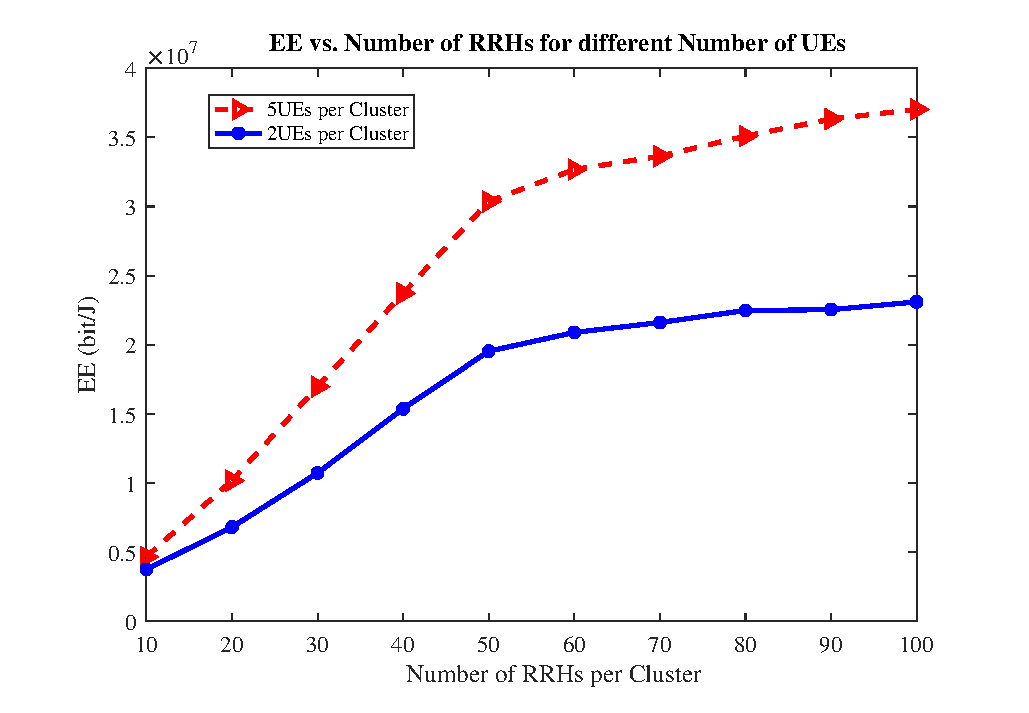
\includegraphics[width=\linewidth, height=12cm]{./fig3/rrh}
  \caption{
  بازدهی انرژی با توجه به تغییرات تعداد واحدهای رادیویی در هر خوشه برای توان بهینه برای 
   دو کاربر مختلف
   و پارامترهای جدول \ref{tab:title}}
  \label{fig:nem1}
\end{figure}
 در شکل \ref{fig:nem1}، بازدهی انرژی سیستم \lr{MIMO C-RAN} بر اساس تعداد واحدهای رادیویی در هر خوشه برای الگوریتم مورد استفاده و برای دو تعداد کاربر متفاوت، رسم شده است. 
 همانطور که  شکل  نشان می دهد، با افزایش تعداد واحدهای رادیوی، بازدهی انرژی افزایش می یابد و سپس  در این شکل از حدود 50 واحد رادیویی شیب افزایش بازدهی انرژی کمتر شده و به نظر می آید که رو به ثابت شدن است زیرا با افزایش واحد های رادیویی ابتدا نرخ ارسال داده بیشتر می شود و بازدهی انرژی بهبود می یابد و در نهایت نرخ ارسال داده دیگر بیشتر نمی گردد و ثابت می شود. زیرا در اینجا با افزایش تعداد واحدهای رادیویی، مجموع توان کل افزایش می یابد در نتیجه نرخ انتقال داده نیز بیشتر می گردد.

  \begin{figure}[h]
  \centering
    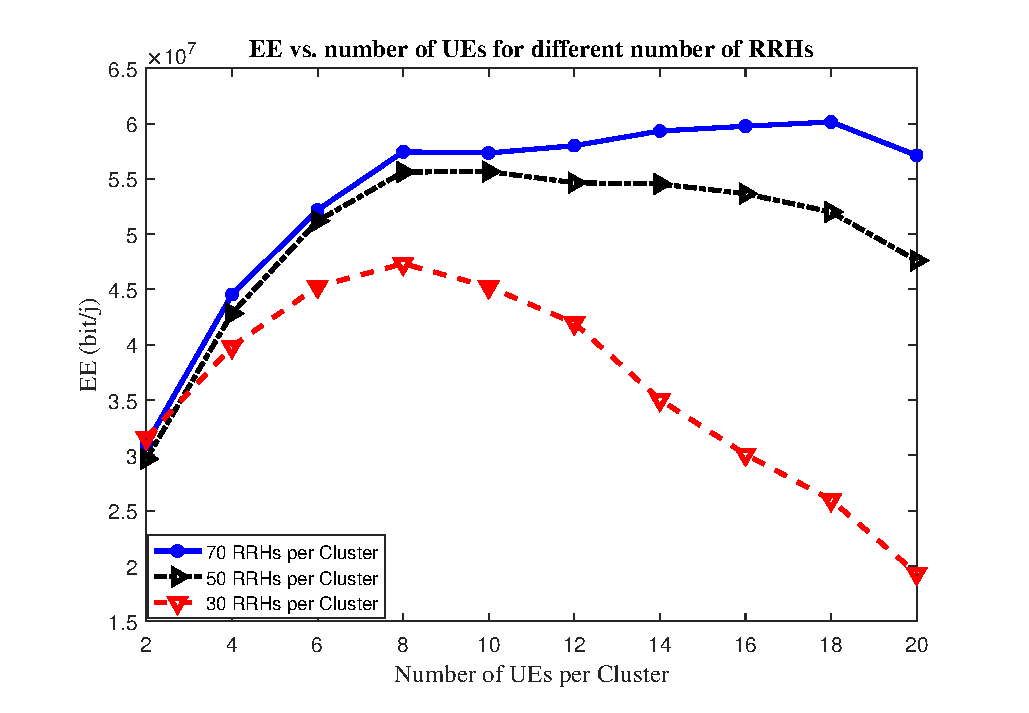
\includegraphics[width=\linewidth]{./fig3/ueEnd}
  \caption{  بازدهی انرژی با توجه به تغییرات تعداد کاربران در هر خوشه برای توان بهینه  برای 
   سه واحد رادیویی مختلف
   و پارامترهای جدول \ref{tab:title} و $P_c = 9dbm$}
  \label{fig:nem2}
\end{figure}


در شکل \ref{fig:nem2}، بازدهی انرژی بر اساس تعداد کاربران در هر خوشه برای الگوریتم مورد استفاده و برای سه تعداد واحد رادیویی متفاوت، رسم شده است.همانطور که  دیده می شود با افزایش تعداد کاربران، ابتدا شیب نمودار زیاد می شود و بازدهی انرژی افزایش می یابد زیرا با افزایش کاربران مجموع نرخ های انتقال افزایش می یابد ولی از یک مقدار به بعد تداخل بین کاربران افزایش می یابد و تاثیر خودر را به طور محسوس بر بازدهی انرژی می گذارد و در نتیجه بازدهی انرژی کاهش می یابد. 

%\bibliographystyle{ieeetr}
%\bibliography{bib1}
%\setLTRbibitems
\begin{figure}[H]
  \centering
    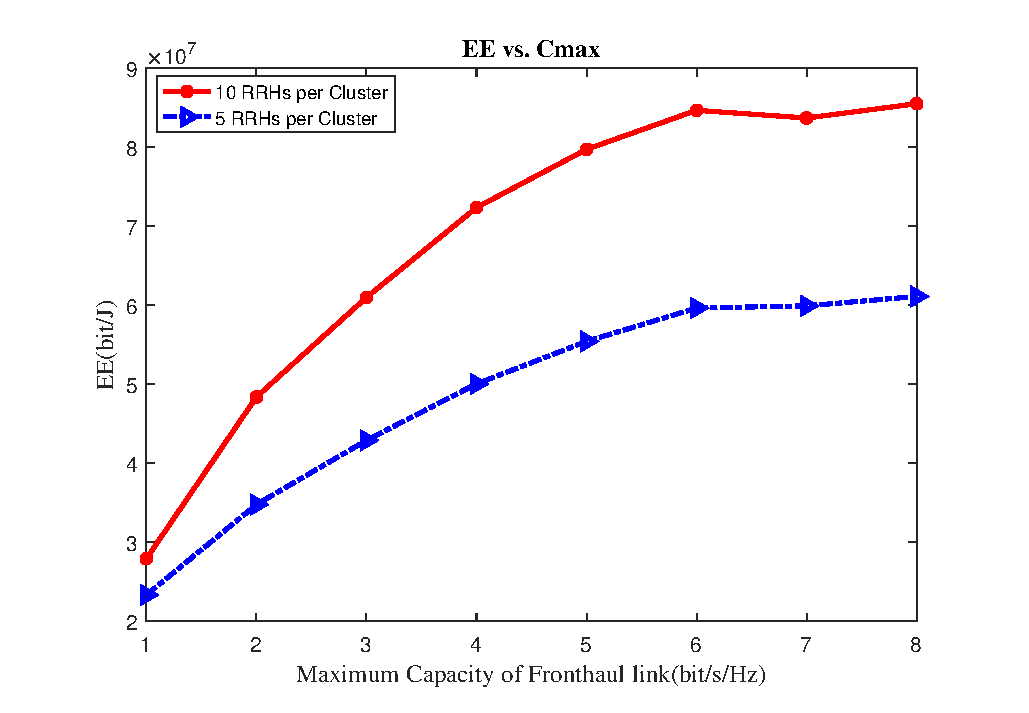
\includegraphics[width=\linewidth]{./fig3/cm}
  \caption{  بازدهی انرژی با توجه به تغییرات $C^{th}$، در در حالت $S =2$, $\text{\lr{Number of RRHs per Cluster}} = 10 , 5$, $\text{\lr{Number of UE per Cluster}} =2$ }
  \label{fig:nem3}
\end{figure}

در شکل \ref{fig:nem3}، بازدهی انرژی بر اساس محدودیت ظرفیت لینک \lr{fronthaul}، برای دو تعداد متفاوت  5 و 10 واحد رادیویی در هر خوشه رسم شده است. با توجه به شکل، زمانی که ظرفیت یک مقداری بیشتر
 می گردد، بدلیل اینکه نرخ قابل دسترس توسط تعداد کاربران و واحدهای رادیویی محدود می گردد، به نظر می آید افزایش محدودیت این ظرفیت تاثیر چندانی در بازدهی انرژی ندارد.  

% \begin{figure}[H]
%  \centering
%    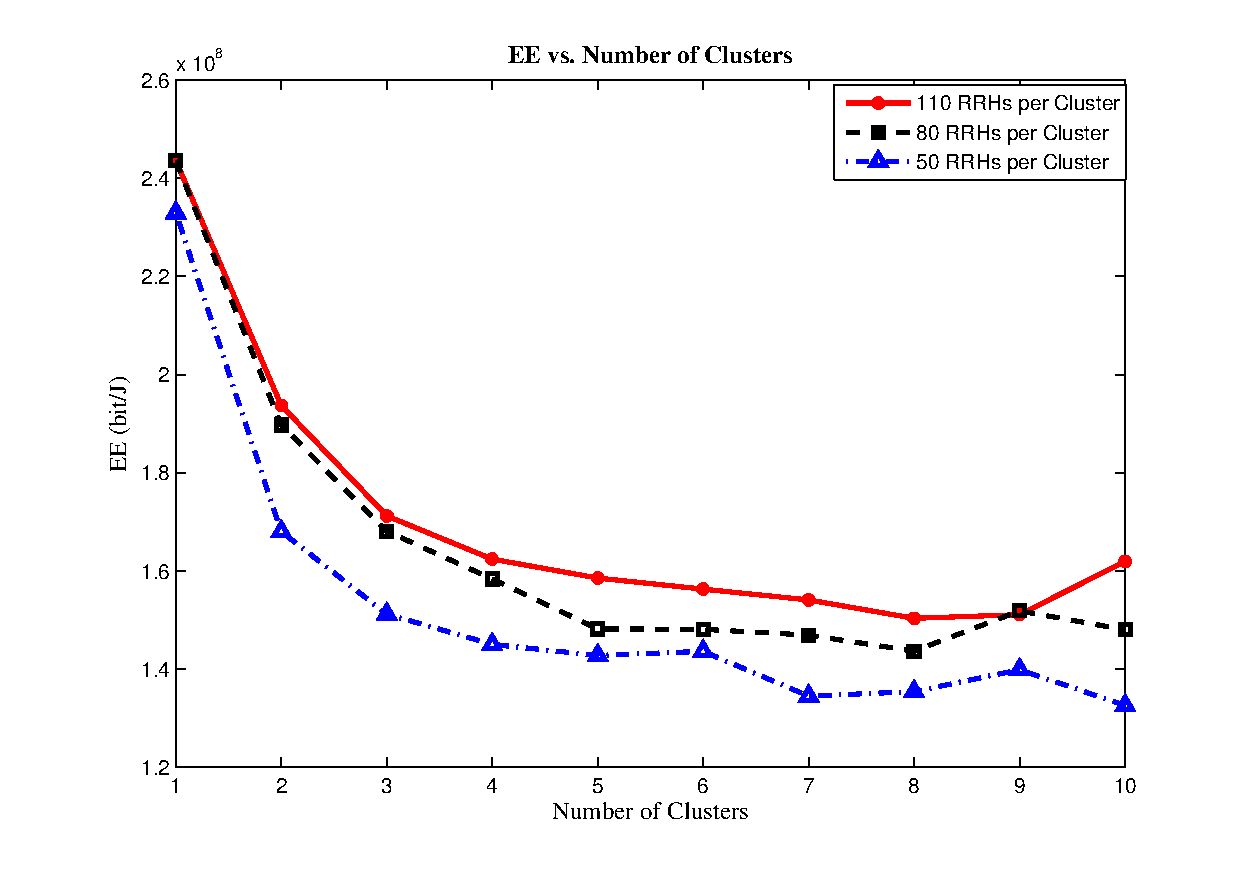
\includegraphics[width=\linewidth]{./fig3/clust}
%  \caption{  بازدهی انرژی بر حسب تعداد خوشه ها برای سه مقدار 50 و 80 و 110 واحد رادیویی}
%  \label{fig:cluster}
%\end{figure}
% حال در شکل \ref{fig:cluster}، بازدهی انرژی بر حسب تعداد خوشه ها برای سه مقدار 50 و 80 و 110 واحد رادیویی در هر خوشه با فرض وجود 3 کاربر در هر خوشه رسم شده است. همانطور که می بینید با افزایش خوشه ها بازدهی انرژی کاهش یافته است.
% 
 
 \begin{figure}[H]
  \centering
    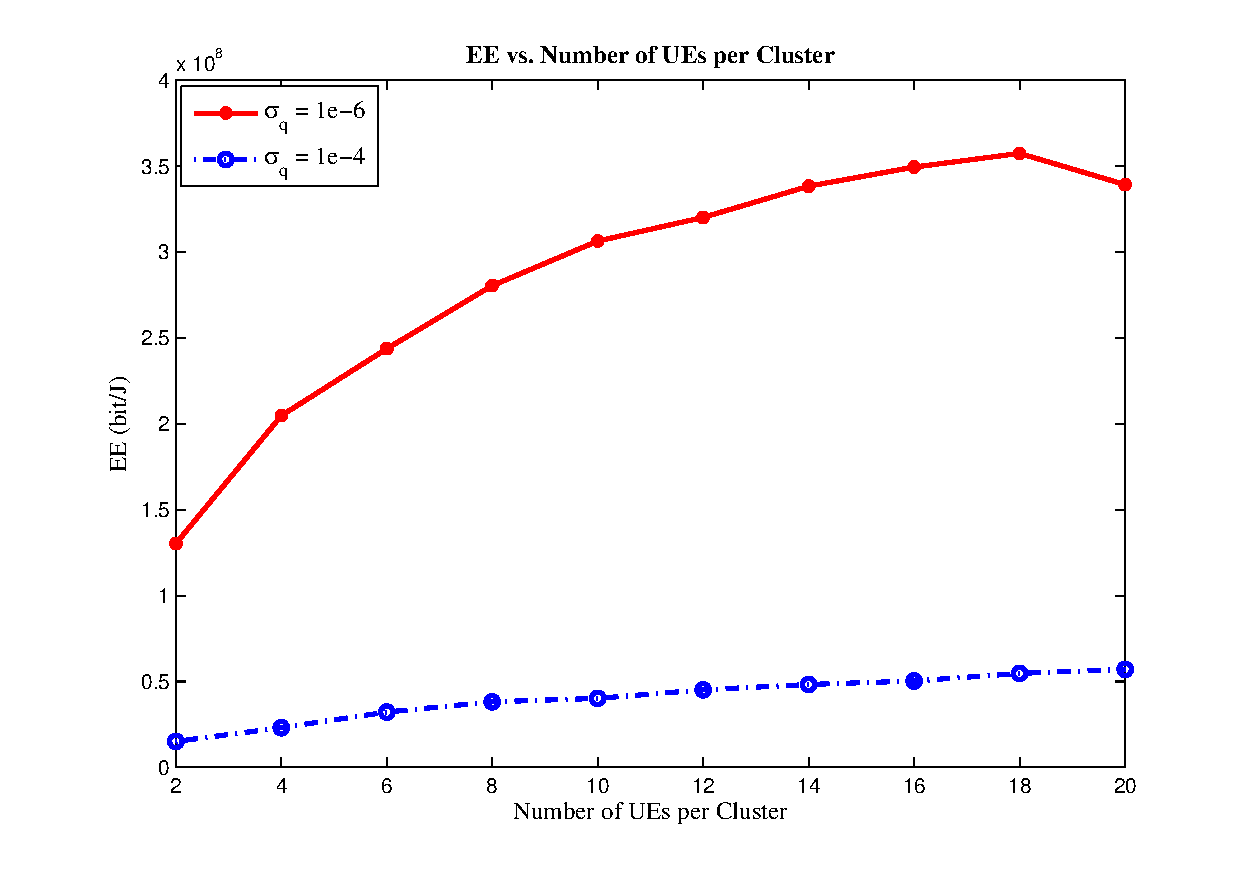
\includegraphics[width=\linewidth]{./fig3/varUE}
  \caption{  بازدهی انرژی بر حسب تعداد کاربران در 3 خوشه  برای دو مقدار 
  $\sigma_q = 1e-4 , 1e-6$
   100 واحد رادیویی
   در هر خوشه}
  \label{fig:Var}
\end{figure}
 حال در شکل \ref{fig:Var}، بازدهی انرژِی بر حسب تعداد کاربران در هر خوشه  برای برای دو مقدار 
  $\sigma_q = 10^{-4} , 10^{-6}$
   و وجود 3 خوشه در هر خوشه با فرض بودن  100 واحد رادیویی در هر خوشه رسم شده است.همانطور که می بینید با افزایش کاربران بازدهی انرژی افزایش یافته است و بازدهی انرژی در واریانس نویز کمتر بشتر از بازدهی انرژی در واریانس نویز بیشتر می باشد.
%    \begin{figure}[H]
%  \centering
%    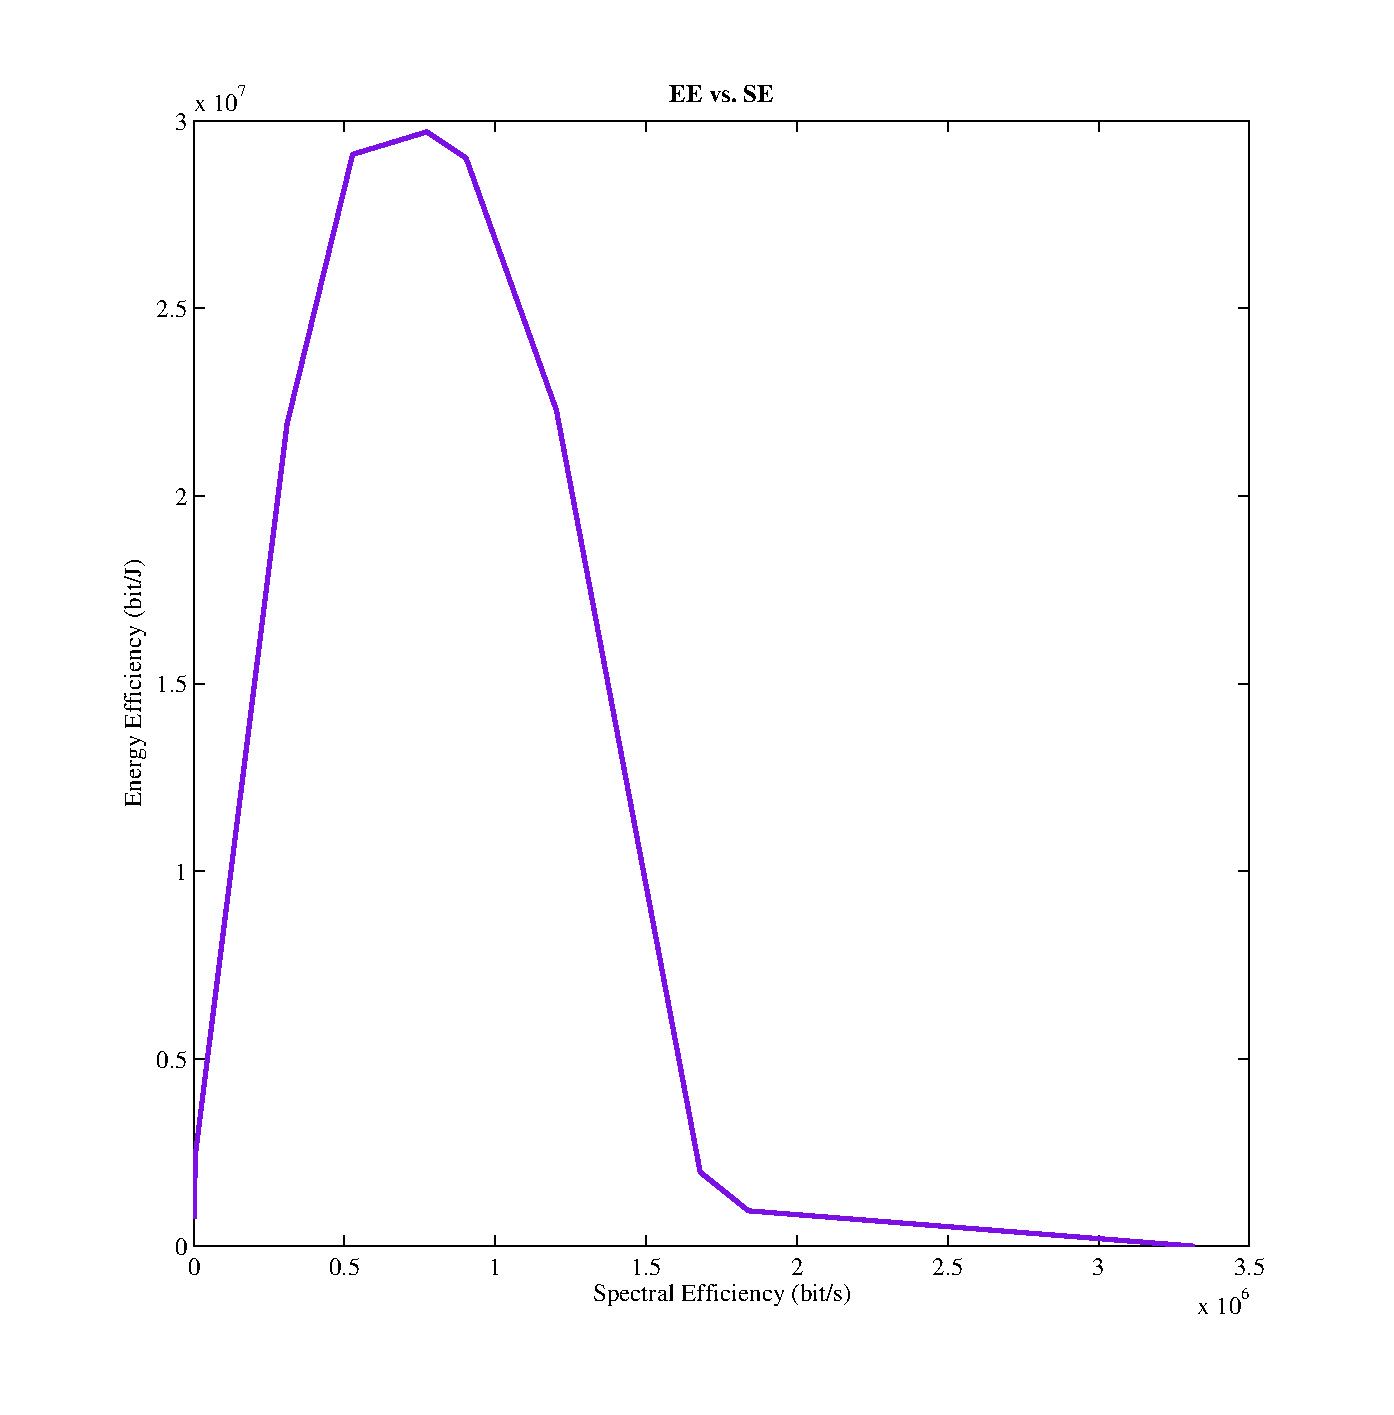
\includegraphics[width=\linewidth]{./fig3/spect}
%  \caption{  بازدهی انرژی بر حسب بازدهی طیف}
%  \label{fig:spect}
%\end{figure}
%در شکل \ref{fig:spect}، بازدهی انرژی بر حسب بازدهی طیف برای 2 خوشه که در هر خوشه 2 کاربر و 10 واحد رادیویی قرار دارد ($\sigma_q = 10^{-4}$)، رسم شده است. این نمودار با تغییر توان بیشینه ی هر واحد رادیویی رسم شده است. ابتدا با افزایش توان از مقدار 0 بازدهی انرژی بر حسب بازدهی طیف زیاد می شود و در نهایت با افزایش توان بازدهی انرژی بر حسب بازدهی طیف کاهش می یابد.  
\subsection{نتیجه گیری}
در این بخش، تخصیص توان بهینه در لینک فروسو برای مدل سیستم \lr{MIMO C-RAN} با فرض محدودیت بر روی ظرفیت \lr{fronthaul}، در نظر گرفته شده است. مدل سیستم شرح داده شده و مسئله ی تخصیص توان بهینه با روش الگوریتم بهینه و استفاده از تابع لاگرانژ حل شده است. شبیه سازی ها نشان می دهد که با افزایش تعداد واحدهای رادیویی عملکرد سیستم بهبود داده و افزایش تعداد کاربران ابتدا منجر به افزایش بازدهی انرژی می گردد و سپس به دلیل زیاد شدن تاثیر تداخل، \lr{EE} کاهش می یابد. همچنین با کاهش نویز کوانتیزاسیون عملکرد سیستم بهبود می یابد. علاوه بر این، با افزایش  بیشینه ظرفیت لینک \lr{fronthaul} ابتدا بازدهی انرژی زیاد شده سپس شیب افزایش بازدهی انرژی، کم می شود.
%%%%%%%%%%%%%%%%%%%%%%%%%%%%%%%%%%%%%%%%%%%%%%%%%
\section{لینک فراسو}
در این بخش، لینک فراسو برای سیستم \lr{MIMO C-RAN} در نظر گرفته شده است که  پیام در مسیر لینک فراسو از کاربر به واحدهای رادیویی منتقل می شود و پس از فشرده سازی توسط لینک \lr{fronthaul} به واحد کنترل منتقل می گردد. \newline
همانند لینک فروسو فرض بر این است که واحدهای رادیویی و کاربران خوشه بندی شده اند به طوری که هر خوشه  شامل تعدادی واحد رادیویی است که به کاربران موجود در آن خوشه، سرویس دهی می کنند.

 \begin{figure}
  \centering
    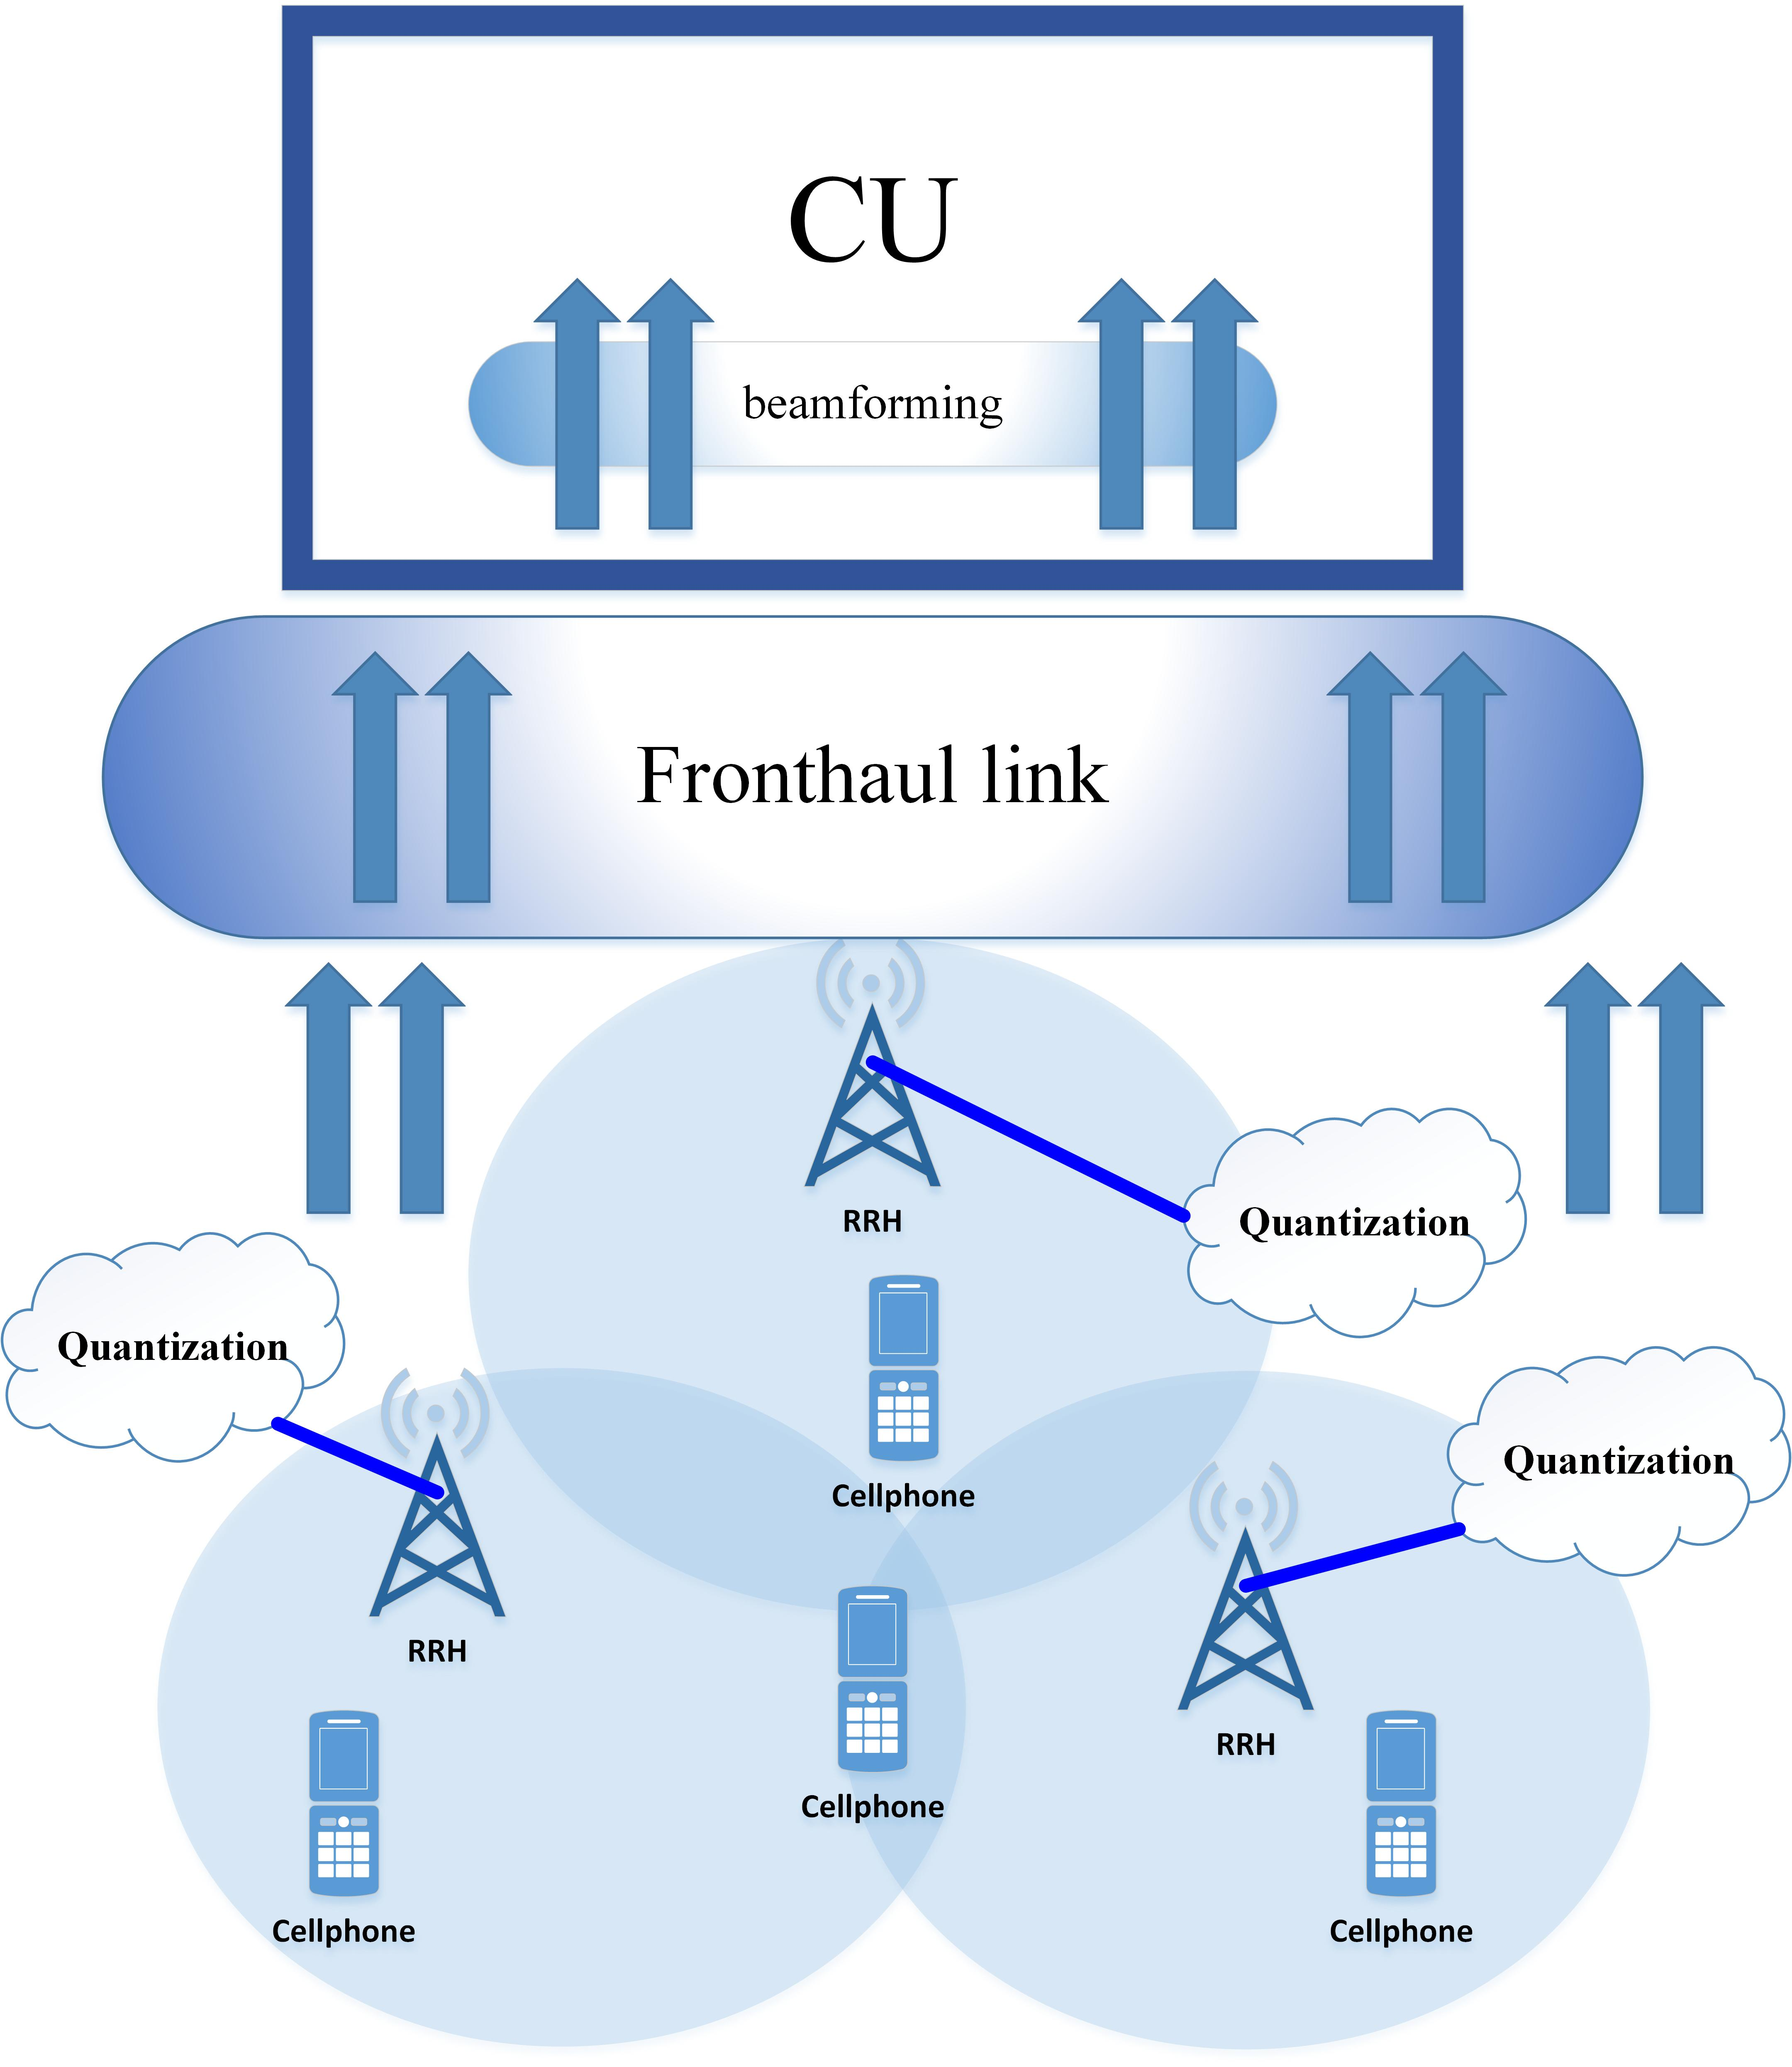
\includegraphics[scale = 0.45]{./fig/Drawing2}
  \caption{ساختار 
  \lr{C-RAN}
  در  لینک فراسو
  }
  \label{fig:cr2}
\end{figure}
همچنین در این مدل از روش پرتو دهی برای کاهش تداخل استفاده می کنیم که پرتو دهی در داخل واحد کنترل صورت می گیرد.
در ادامه، ابتدا سیستم  مدل و سپس نرخ قابل دسترسی بیان شده و مسئله ی تخصیص توان بررسی می گردد.
\subsection{مدل سیستم}
مدل سیستم برای لینک فراسو نیز همانند لینک فروسو می باشد که در ادامه شرح داده شده است\cite{ofdma,ulCompression}.
 سیستم \lr{MIMO C-RAN} شامل $R$ واحد رادیویی می باشد که $D$ کاربر تک آنتنه را سرویس می دهند.فرض بر این است که کاربران و واحد رادیوییها، به 
 $S$
خوشه تقسیم شده اند که $v$ امین خوشه،
 دارای $R_v$ واحد رادیویی است که ${D}_v$ کاربر را سرویس دهی می کنند.
 علاوه بر این، فرض بر این است که
$j$
امین واحد رادیویی، در $v$امین خوشه، توسط لینک فیبر نوری با ظرفیت محدود $c_{r_{(v,j)}}$ به واحد کنترل متصل می گردد.
\begin{equation}
\begin{split}
\mathcal{R}_v= \{  r_{(v,i)} | 1 \leq i \leq {R}_v , i\in Z^+\}, \\
\mathcal{C}_{\mathcal{R}_v}= \{C_{r_{(v,j)}}| 1 \leq j \leq {R}_v , j\in Z^+\}, \\
\mathcal{D}_v= \{  d_{(v,k)} | 1 \leq k \leq {D}_v , k\in Z^+\},  \\
\end{split}
\end{equation} 
که
 $\mathcal{R}_v$، $\mathcal{C}_{\mathcal{R}_v}$
 و
  $\mathcal{D}_v$
 به ترتیب نشان دهنده ی دسته واحد رادیوییها، دسته ی ظرفیت لینک \lr{Fronthaul} و دسته ی کاربران در $v$امین دسته ی خوشه می باشد.\newline
واحد رادیویی
ها تداخل پیام ها را از خوشه های دیگر نیز دریافت می کنند.\newline
 \subsection{آنالیز نرخ قابل دسترس}
در این قسمت، هدف بررسی نرخ قابل دسترسی سیستم می باشد.
\begin{theorem}\label{t1}
 نرخ قابل دسترسی برای کاربر $d_{(s,k)}$ به صورت زیر می باشد:
\begin{equation}\label{e1}
\mathfrak{R}_{d_{(s,k)}} = B \log_2(1+\gamma_{d_{(s,k)}}),
\end{equation}
که $B$ پهنای باند کانال و $\gamma_{d_{(s,k)}}$ همان \lr{SINR} دریافتی $k$امین کاربر در $s$امین دسته ی خوشه است که به صورت زیر بیان می گردد.  
\begin{equation}\label{5}
\gamma_{d_{(s,k)}}= \frac{p_{d_{(s,k)}} |{\boldsymbol{w}^H}_{\mathcal{R}_{s},d_{(s,k)}}^آ\boldsymbol{h}_{\mathcal{R}_s, d_{(s,k)}}|^2}{I_{d_{(s,k)}}+B\nu}.
\end{equation}
در فرمول \eqref{5}، 
$I_{d_{(s,k)}}$
نشان دهنده ی توان سیگنال تداخلی است.$B\nu$
نشان دهنده ی توان نویز است و
$\boldsymbol{h}_{\mathcal{R}_s, d_{(s,k)}}$ 
 نشان دهنده ی بردار کانال بین $k$امین کاربر و واحدهای رادیویی
 $s$
 امین دسته ی خوشه می باشد. همچنین 
 $\boldsymbol{w}_{\mathcal{R}_{s},d_{(s,k)}}$
 نشان دهنده ی بردار پرتو دهی استفاده شده در $s$امین دسته ی خوشه ها برروی واحدهای رادیویی برای بدست آوردن پیام $k$امین کاربر می باشد. 
 $p_{d_{(s,k)}}$
 توان ارسالی$k$امین کاربر در $s$امین دسته ی خوشه می باشد.
\end{theorem}
\begin{proof}
در این قسمت می خواهیم $\gamma$ را بدست آوریم

فرض کنید $\boldsymbol{y}_{\mathcal{R}_s}$ یک بردار
 $R_s \times 1$
باشد که نشان دهنده ی سیگنال دریافتی توسط دسته ای از واحدهای رادیویی در $s$
امین خوشه باشد که به صورت زیر بدست می آید.
\begin{equation} \label{1}
\boldsymbol{y}_{\mathcal{R}_s} = \sum_{v=1}^S \boldsymbol{H}_{\mathcal{R}_v,\mathcal{D}_s}{\boldsymbol{x}}_{\mathcal{D}_v}+ \boldsymbol{z}_{\mathcal{D}_s},
\end{equation}
که   ${\boldsymbol{x}}_{ \mathcal{D}_v} = [{x}_{ d_{(v,1)}},...,{ x}_{ d_{(v,\mathcal{D}_v)}}]^T \in \mathbb{C}^{{D}_v } $ 
بردار سمبل ارسالی خوشه ی  $v$ ام می باشد.\newline
 $\boldsymbol{z_{\mathcal{D}_s}} \backsim \mathcal{N}(0,N_0\boldsymbol{I}_{{D}_s})$ 
 نویز گوسی سفید اضافه شونده می باشد که دارای توان $N_0$
 و \newline
 $\boldsymbol{H}_{\mathcal{R}_v,\mathcal{D}_s}  \in \mathbb{C}^{{R}_v\times {D}_s}$ 
 نشان دهنده ی ماتریس کانال بین  کاربران $\mathcal{D}_s$ در دسته ی
 $s$
   ام و واحدهای رادیویی   $\mathcal{R}_v$ در دسته ی   $v$ ام می باشد.\newline
همچنین مدل کانال همانند لینک فروسو با توجه به فرمول \eqref{channel}، بدست می آید.
 حال می خواهیم پیام دریافتی توسط واحد رادیویی  $n$ ام در دسته ی $s$ ام را بدست آوریم:
 
\begin{equation} \label{100}
y_{r_{(s,n)}} = \sum_{k=1}^{D_s} h_{r_{(s,n)},d_{(s,k)}} \sqrt{p_{d_{(s,k)}}}  x_{d_{(s,k)}}
+\sum_{t=1,t\neq s}^{S} \sum_{j=1}^{D_t} h_{r_{(s,n)},d_{(t,j)}} \sqrt{p_{d_{(t,j)}}} x_{d_{(t,j)}}
 +z_{r_{(s,n)}}
\end{equation}
پیام دریافتی توسط واحد رادیویی، بعد از فشرده سازی به صورت زیر می شود
\begin{equation}
\hat{y}_{r_{(s,n)}} = y_{r_{(s,n)}} + q_{r_{(s,n)}} 
\end{equation}
پیام هر کاربر در واحد کنترل با اعمال پرتو دهی \LTRfootnote{beamforming} به صورتی که در ادامه بیان شده، بدست می آید

\begin{equation}
\begin{split}
\hat{x}_{d_{(s,k)}} = & {\boldsymbol{w}^H}_{\mathcal{R}_s, d_{(s,k)}} \boldsymbol{h}_{\mathcal{R}_s, d_{(s,k)}} \sqrt{p_{d_{(s,k)}}}  x_{d_{(s,k)}} \\
+ & \sum_{i=1,i\neq k}^{D_s}  {\boldsymbol{w}^H}_{\mathcal{R}_s, d_{(s,k)}} \boldsymbol{h}_{\mathcal{R}_s, d_{(s,i)}} \sqrt{p_{d_{(s,i)}}}  x_{d_{(s,i)}} \\
+&  \sum_{t=1,t\neq s}^{S} \sum_{j=1}^{D_t} {\boldsymbol{w}^H}_{\mathcal{R}_s, d_{(s,k)}} \boldsymbol{h}_{\mathcal{R}_s, d_{(t,j)}} \sqrt{p_{d_{(t,j)}}}  x_{d_{(t,j)}} \\
+& {\boldsymbol{w}^H}_{\mathcal{R}_s, d_{(s,k)}}  ({\boldsymbol{q}}_{\mathcal{R}_s} + {\boldsymbol{z}}_{\mathcal{R}_s})
\end{split}
\end{equation}
حال برای بدست آوردن  \lr{SINR}، توان سیگنال بر روی توان تداخل و نویز را بدست می آوریم:
\begin{equation}
\gamma = \frac{p_{d_{(s,k)}}|{\boldsymbol{w}^H}_{\mathcal{R}_s, d_{(s,k)}} \boldsymbol{h}_{\mathcal{R}_s, d_{(s,k)}}|^2}{
  I_{d_{(s,k)}}
+ B \times \nu_{d_{(s,k)}}
}
\end{equation}
که داریم :
\begin{equation}
\begin{split}
\nu_{d_{(s,k)}}&  = {\boldsymbol{w}^H}_{\mathcal{R}_s, d_{(s,k)}}  (diag({\sigma_n^2}_{r_{(s,1)}}...{\sigma_n^2}_{r_{(s,R_s)}})+diag({\sigma_q^2}_{r_{(s,1)}}...{\sigma_q^2}_{r_{(s,R_s)}})) {\boldsymbol{w}}_{\mathcal{R}_s, d_{(s,k)}}\\
I_{d_{(s,k)}}& = \sum_{i=1,i\neq k}^{D_s}  |{\boldsymbol{w}^H}_{\mathcal{R}_s, d_{(s,k)}} \boldsymbol{h}_{\mathcal{R}_s, d_{(s,i)}}|^2 p_{d_{(s,i)}} +\sum_{t=1,t\neq s}^{S} \sum_{j=1}^{D_t} |{\boldsymbol{w}^H}_{\mathcal{R}_s, d_{(s,k)}} \boldsymbol{h}_{\mathcal{R}_s, d_{(t,j)}}|^2 p_{d_{(t,j)}} 
\end{split}
\end{equation}
 در اینجا  $\sigma_n^2$ واریانس نویز می باشد که  برای سادگی برای همه ی واحدهای رادیویی ثابت فرض شده و  دارای مقدار $N_0$ 
است و $\sigma_q^2$ واریانس نویز فشرده سازی می باشد.
علاوه بر این با استفاده از پرتودهی \lr{MMSE}، ماتریس پرتودهی به صورت زیر است 
\begin{equation}
\boldsymbol{W}_{\mathcal{R}_s,\mathcal{D}_s} = \hat{\boldsymbol{H}}_{\mathcal{R}_s,\mathcal{D}_s}(\hat{\boldsymbol{H}}_{\mathcal{R}_s,\mathcal{D}_s}^H \hat{\boldsymbol{H}}_{\mathcal{R}_s,\mathcal{D}_s}+ \alpha \boldsymbol{I}_{{D}_s})^{-1},
\end{equation} 
همچنین  $\alpha$، فاکتور رگولاریزاسیون است در صورتی که $\alpha$ صفر یاشد، ماتریس پرتو دهی \lr{ZF} خواهیم داشت.
\end{proof}
\subsection{بهینه سازی تخصیص توان}
در این قسمت می خواهیم توان را طوری اختصاص دهیم تا بازدهی انرژی به بیشینه مقدار خود برسد.
می دانیم نرخ قابل دسترس بر روی لینک \lr{fronthaul}، بین $n$ امین واحد رادیویی در $s$ امین خوشه  و  واحد کنترل به صورت زیر بدست می آید 
\begin{equation}
C_{r_{(s,n)}} = \log{\frac{1+( \sum_{k=1}^{D_s}|h_{r_{(s,n)},d_{(s,k)}}|^2{p_{d_{(s,k)}}} + \sum_{t=1,t\neq s}^{S}\sum_{l=1}^{D_t}|h_{r_{(s,n)},d_{(t,l)}}|^2{p_{d_{(t,l)}}}+ B N_0) }{ \sigma_{q_{(s,n)}}^2})},
\end{equation}
\subsubsection{شرح مسئله}
 همانطور که گفته شد نسبت مجموع نرخ ها در سیستم به کل توان ارسالی کاربرها نشان دهنده ی بازدهی انرژی است که با $\eta$ نمایش داده می شود و می توان اینگونه بیان کرد
\begin{equation}\label{eta1}
\eta(\boldsymbol{P}) := \frac{\sum\limits_{s=1}^{S} \sum\limits_{k=1}^{{D}_s}\mathfrak{R}_{d_{(s,k)}} }{\sum\limits_{s=1}^{S} \sum\limits_{k=1}^{{K}_s}{p}_{d_{(s,k)}}} = \frac{R_{total}(\boldsymbol{P})}{P_{UE}(\boldsymbol{P})},
\end{equation}
که در اینجا  $ \boldsymbol{P} = \{ \boldsymbol{P}_{\mathcal{D}_s}|  1 \leq s \leq S, s \in \mathbb{Z}^{+} \}$ ماتریس تخصیص توان است. در این بخش، بیشینه سازی بازدهی انرژی با شروط زیر مورد بررسی قرار می گیرد 
\begin{equation}\label{p11}
\begin{aligned}
\max\limits_{\boldsymbol{P}}   \quad &   \eta(\boldsymbol{P})\\
\text{\lr{subject to}} \quad  &  0 \leq {p}_{d_{(s,k)}} \leq P_{max} && \qquad \forall s, \forall k,   \\
&\mathfrak{R}_{d_{(s,k)}} \geq  \mathfrak{R}_{d_{(s,k)}}^{th} && \qquad \forall s, \forall k, \\ 
&C_{r_{(s,i)}} \leq C_{r_{(s,i)}}^{th}  &&\qquad \forall s, \forall i, \\
\end{aligned}			
\end{equation}
همانند لینک فروسو، بدلیل محدب نبودن مسئله از روش الگوریتم تکرار شونده استفاده می کنیم.
\subsection{روش مورد استفاده}
در این قسمت، به جای ماکسیمم کردن \eqref{eta1}، همانند لینک فروسو، از قضیه ی \eqref{t2} استفاده می نماییم.
 همچنین کران بالایی برای تداخل بدست می آید که در ادامه بیان می شود.
\begin{equation} \label{id}
\tilde{I}_{d_{(s,k)}} = \sum_{v=1}^{S}  |{\boldsymbol{w}^H}_{\mathcal{R}_s, d_{(s,k)}} \boldsymbol{h}_{\mathcal{R}_v, d_{(s,i)}}|^2 P_{max} 
\end{equation}
در نتیجه با توجه به رابطه ی  \eqref{id}، می توان $\gamma$ را به این صورت تخمین زد:
\begin{equation}
\tilde{\gamma}_{d_{(s,k)}}= \frac{p_{d_{(s,k)}} |{\boldsymbol{w}^H}_{\mathcal{R}_{s},d_{(s,k)}}^آ\boldsymbol{h}_{\mathcal{R}_s, d_{(s,k)}}|^2}{\tilde{I}_{d_{(s,k)}}+B\nu}.
\end{equation}
ابتدا تابع لاگرانژ را تشکیل می دهیم تا بتوان با استفاده از آن، از الگوریتم تکرار شونده ی \eqref{alg}، استفاده کرد. 
\begin{equation}
\begin{split}
\mathcal{L}(\boldsymbol{P}; \boldsymbol{\lambda}, \boldsymbol{\mu}, \boldsymbol{ \kappa}) & = \sum\limits_{s=1}^{S} \sum\limits_{k=1}^{\mathcal{D}_s}\mathfrak{\tilde{R}}_{d_{(s,k)}} 
- \eta \sum\limits_{s=1}^{S} \sum\limits_{k=1}^{\mathcal{K}_s}{p}_{d_{(s,k)}}\\
&+\sum\limits_{s=1}^{S} \sum\limits_{k=1}^{\mathcal{D}_s} \lambda_{d_{(s,k)}} (\mathfrak{\tilde{R}}_{d_{(s,k)}}-\mathfrak{R}_{d_{(s,k)}}^{th})\\
&- \sum\limits_{s=1}^{S} \sum\limits_{k=1}^{\mathcal{K}_s} \mu_{d_{(s,k)}} ({p}_{d_{(s,k)}}-P_{max})\\
&- \sum\limits_{s=1}^{S} \sum\limits_{i=1}^{\mathcal{R}_s} \kappa_{r_{(s,i)}} (C_{r_{(s,i)}}-C_{r_{(s,i)}}^{th}).\\
\end{split}
\end{equation}
که در اینجا، $\boldsymbol{\lambda}, \boldsymbol{\mu}, \boldsymbol{\kappa} \geq 0$
بردارهای ضرایب لاگرانژ می باشد .\newline
با استفاده از این معادله و مشتقگیری از آن، توان بهینه به صورت زیر بدست می آید
\begin{equation}
p_{d_{(s,k)}}^* \approx [\frac{ B(1+\lambda_{d_{(s,k)}} )-(\sum_{n=1}^{\mathcal{R}_s}\kappa_{r_{(s,i)}})}{\ln2 \times (\eta + \mu_{d_{(s,k)}})}]^+;
\end{equation} 

  در آخر، برای بدست آوردن توان بهینه، الگوریتم \eqref{alg1} مورد استفاده قرار می گیرد \cite{hcranEE}
 \begin{latin}
\begin{algorithm}
\caption{Energy-Efficient Power Allocation}\label{alg1}
\begin{algorithmic}

\State Set the maximum number of iterations $I_{max}$, convergence condition $\epsilon_{\eta}$  and the initial value $\eta^{(1)} = 0$
\State Set the iteration index $i = 1$ and begin the iteration (Outer
Loop).
\For {$ 1\leq i \leq  Imax$}
\State Solve the resource allocation problem with $\eta^{(i)}$ (Inner Loop);
\State Obtain $P^{(i)}, R_{total}^{(i)}, P_{UE}^{(i)}$
\If {$ R_{total}(\boldsymbol{P}^{(i)}) - \eta^{(i)} P_{UE}(\boldsymbol{P}^{(i)}) < \epsilon_{\eta} $} 
\State Set $\boldsymbol{P}^*= \boldsymbol{P}^{(i)} $   and  $ \eta^{*} =\eta^{(i)} $;
\State break;
\Else
\State Set $\eta^{(i)}= \frac{R_{total}(\boldsymbol{P}^{(i))}}{P_{UE}(\boldsymbol{P}^{(i))}}$ and $i= i+1$;
\EndIf 
\State \textbf{end if}
\EndFor 
\State \textbf{end for}

\end{algorithmic}
\end{algorithm}
\end{latin}
\subsection{نتایج عددی}
در این بخش، نتایج عددی الگوریتم مورد استفاده را برای سیستم \lr{MIMO C-RAN} با پارامترهای بیان شده در جدول \ref{tab:title3} و استفاده از پرتو دهی \lr{ZF} بیان می شود.
\begin{latin} 
 \begin{table}[H]
 \caption {\rl{پارامترهای شبیه سازی}} \label{tab:title3} 
 \begin{center}
  \begin{tabular}{||c c ||} 
  \hline
  Parameter & Value \\ [0.5ex] 
  \hline\hline
  Number of cluster S & 3 \\ 
  \hline
  Noise power density & -174dBm/Hz\\
  \hline
  Bandwidth & 120KHz \\
  \hline
 Maxmimun transmit Power & 10dBm \\
  \hline
  Circuit Power of whole RRHs & 10dBm \\
  \hline
  Variance of quantization noise & $10^{-2}$ \\
  \hline
   Maxmimun fronthaul link's rate & 20bits/sec/Hz \\
  \hline
  Minimum data rate &  1bits/sec/Hz \\ [1ex] 
  \hline
 \end{tabular}
 \end{center}
 \end{table}
 \end{latin}
  \begin{figure}[H]
  \centering
    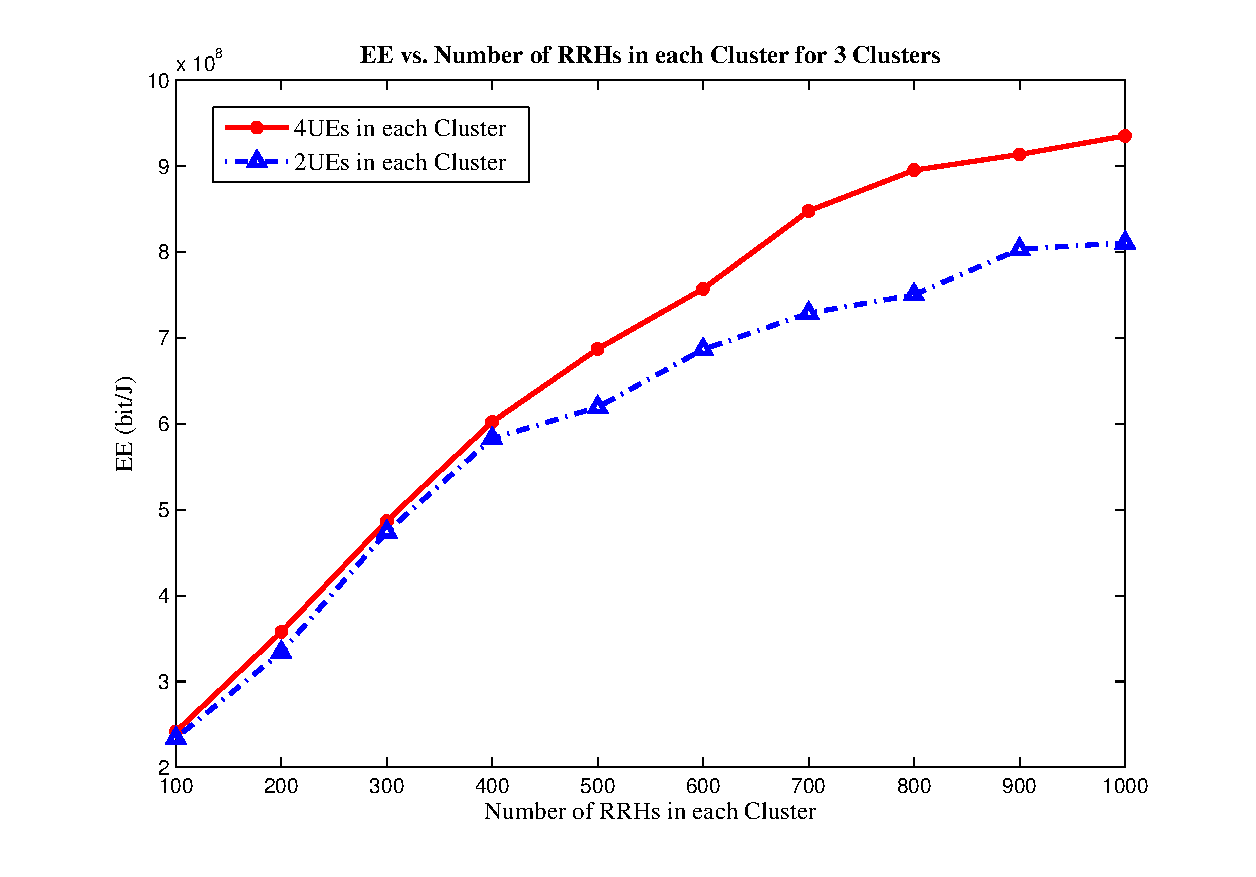
\includegraphics[width=\linewidth, height=12cm]{./fig3/rrhul}
  \caption{
  بازدهی انرژی با توجه به تغییرات تعداد واحدهای رادیویی  در هر خوشه برای توان بهینه  برای 
   دو کاربر مختلف
   و پارامترهای جدول \ref{tab:title3}}
  \label{fig:rrhul}
\end{figure}
 در شکل \ref{fig:rrhul}، بازدهی انرژی سیستم \lr{MIMO C-RAN} بر اساس تعداد واحدهای رادیویی در هر خوشه برای الگوریتم مورد استفاده و برای دو تعداد کاربر متفاوت، رسم شده است. 
 همانطور که  شکل  نشان می دهد، با افزایش تعداد واحدهای رادیوی، بازدهی انرژی افزایش می یابد و از یک مقدار به بعد شیب افزایش بازدهی انرژی کمتر شده است. زیرا با افزایش تعداد واحدهای رادیویی، مجموع توان کل افزایش یافته و در نتیجه نرخ انتقال داده نیز بیشتر می گردد.

 \begin{figure}[H]
  \centering
    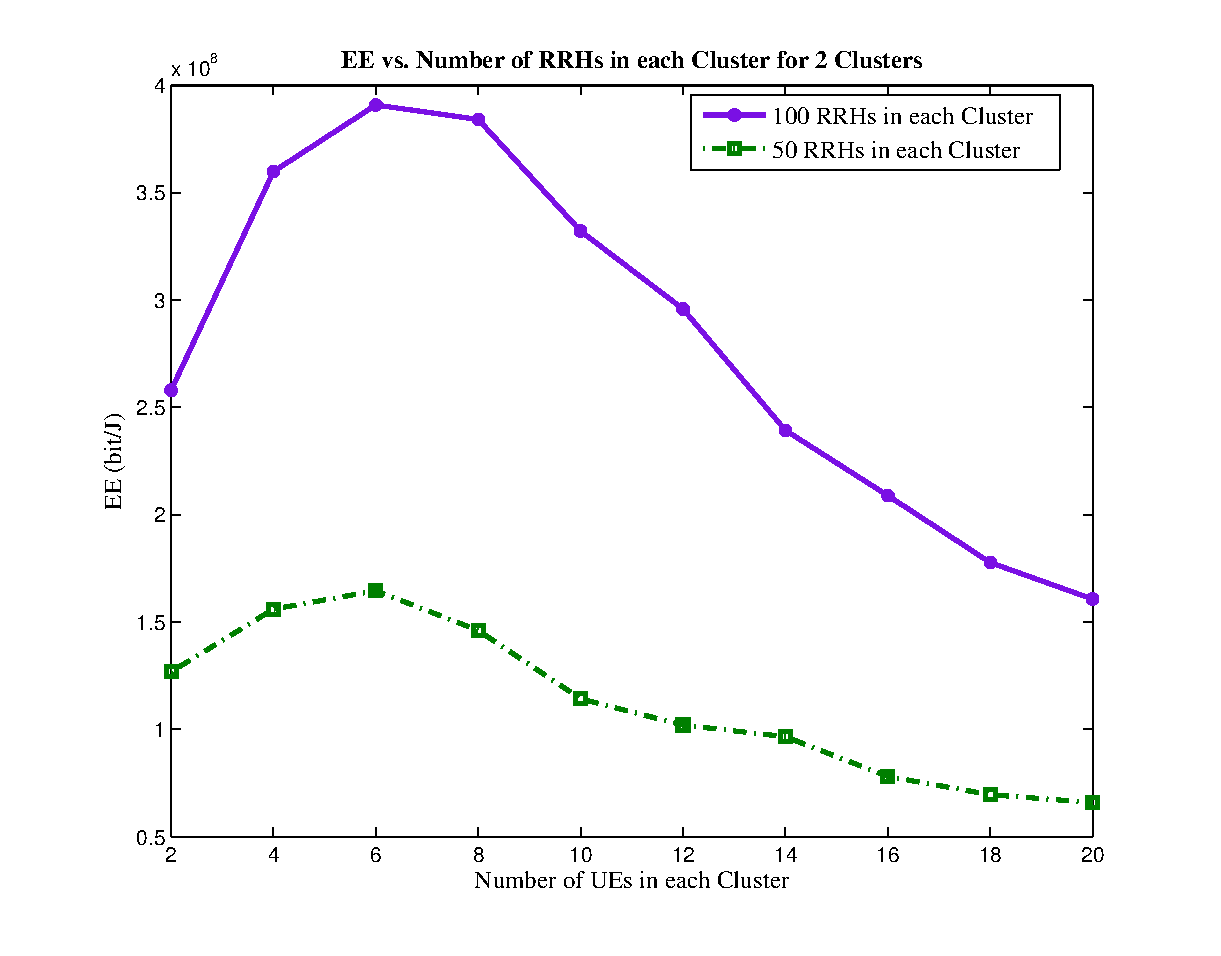
\includegraphics[width=\linewidth]{./fig3/ueul}
  \caption{  بازدهی انرژی با توجه به تغییرات تعداد کاربران در هر خوشه برای توان بهینه برای 
   دو واحد رادیویی مختلف
   و پارامترهای جدول \ref{tab:title3} و $S=2$}
  \label{fig:ueul}
\end{figure}


در شکل \ref{fig:ueul}، بازدهی انرژی بر اساس تعداد کاربران در هر خوشه برای الگوریتم مورد استفاده و برای دو تعداد واحد رادیویی متفاوت، رسم شده است. همانطور که  دیده می شود با افزایش تعداد کاربران، ابتدا شیب نمودار زیاد می شود و بازدهی انرژی افزایش می یابد سپس به دلیل افزایش تاثیر تداخل بین کاربران بازدهی انرژی کاهش می یابد. 

\begin{figure}[H]
  \centering
    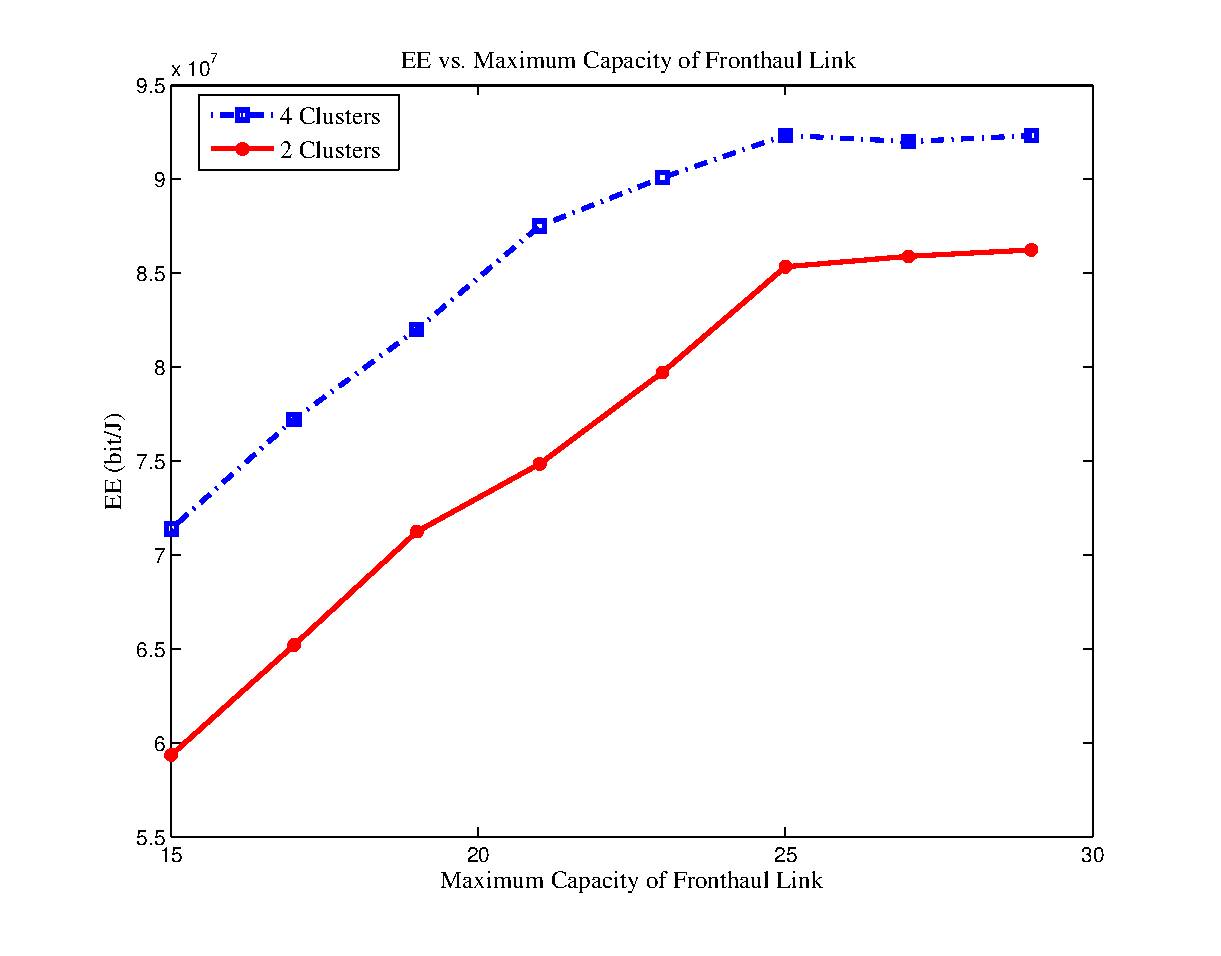
\includegraphics[width=\linewidth]{./fig3/cap}
  \caption{  بازدهی انرژی با توجه به تغییرات $C^{th}$، در در حالت $S =2 ,4 $, $\text{\lr{Number of RRHs per Cluster}} = 30$, $\text{\lr{Number of UE per Cluster}} =2$ }
  \label{fig:cap}
\end{figure}

در شکل \ref{fig:cap}، بازدهی انرژی بر اساس محدودیت ظرفیت لینک \lr{fronthaul}، برای دو تعداد متفاوت  2 و 4 خوشه و در هر خوشه 2 کاربر و 30 واحد رادیویی رسم شده است. با توجه به شکل، ابتدا با بازدهی انرژی، افزایش یافته،
سپس بدلیل اینکه نرخ قابل دسترس توسط تعداد کاربران و واحدهای رادیویی محدود می گردد، به نظر می آید افزایش محدودیت این ظرفیت تاثیر چندانی در بازدهی انرژی ندارد.  
\subsection{نتیجه گیری}
در این بخش، تخصیص توان بهینه در لینک فراسو برای مدل سیستم \lr{MIMO C-RAN} با فرض محدودیت بر روی ظرفیت \lr{fronthaul} و وجود چندین خوشه، در نظر گرفته شده است. مدل سیستم  شرح داده شده و مسئله ی تخصیص توان بهینه با روش الگوریتم بهینه و استفاده از تابع لاگرانژ حل شده است. شبیه سازی ها نشان می دهد همانند لینک فروسو با افزایش تعداد واحدهای رادیویی عملکرد سیستم بهبود داده و افزایش تعداد کاربران منجر به افزایش بازدهی انرژی می گردد ولی در نهایت به دلیل تداخل بازدهی انرژی کاهش می یابد. همچنین، با افزایش  بیشینه ظرفیت لینک \lr{fronthaul} ابتدا بازدهی انرژی زیاد شده سپس شیب افزایش بازدهی انرژی، کم می شود.
%%%%%%%%%%%%%%%%%%%%%%%%%%%%%%%%%%%%%%%%%%%%%%
\chapter{تخصیص منابع در حالت تقسیم زمانی دینامیکی در شبکه دسترسی رادیویی}
\section{مقدمه}
در این فصل هدف بدست آوردن مدل سیستم در حالت تقسیم زمانی یا \lr{TDD} \LTRfootnote{Time Division Duplexing} دینامیکی می باشد که بدین منظور تخصیص توان برای هر دو لینک فراسو و فروسو به طور همزمان بدست می آید.
در تقسیم زمانی دینامیکی، منابع به صورت دینامیکی بین هر دو لینک فراسو و فروسو  تخصیص داده می شود. در سیستم های سنتی  ایستگاه پایه و سیستم سنتی ایستگاه پایه و واحد رادیویی که در فصل اول بیان شد، تداخل بین لینک فراسو و فروسو منجر به کاهش شدید در بازدهی انرژی می گردد در حالی که در سیستم \lr{C-RAN} این تداخل  به دلیل وجود \lr{BBU Pool} و واحد های رادیویی \lr{RRH} و نوع پردازش هایی که در آنها صورت می گیرد، تاثیر چندانی در بازدهی انرژی نمی گذارد \cite{TDD,dynamic}.


حال در ادامه، مدل سیستمی با ساختار \lr{C-RAN}  بیان می نماییم که دارای چندین خوشه است که تعدادی از این خوشه  ها در لینک فراسو و تعدادی دیگر در لینک فروسو عمل می کنند. همچنین تمام واحدهای رادیویی در این خوشه ها به واحد کنترل ابری \lr{BBU Pool} از طریق لینک \lr{fronthaul} با ظرفیت محدود، متصلند. سیگنالهای خوشه های لینک فراسو و فروسو نیز بر یکدیگر تداخل اعمال می کنند.
\section{مدل سیستم}
در این بخش مدل سیستمی برای حالت تقسیم زمانی دینامیکی  براساس معماری \lr{C-RAN} در لینک فراسو و فروسو همانند فصل 3 بیان می شود. فرض بر این است که این سیستم شامل $S$ خوشه می باشد که $S_1$ خوشه در لینک فروسو و $S_2$
 خوشه در لینک فراسو عمل می کنند که :
 $S_1 + S_2 = S$
 است.
 همچنین هر خوشه ی $v$ دارای  $R_v$  واحد رادیویی و $D_v$ کاربر می باشد.  
 علاوه براین، فرض بر این است که
$j$
امین واحد رادیویی، در $v$امین خوشه، توسط لینک فیبر نوری با ظرفیت محدود $C_{r_{(v,j)}}$ به واحد کنترل متصل می گردد. در نتیجه داریم:
\begin{equation}
\begin{split}
\mathcal{R}_v= \{  r_{(v,i)} | 1 \leq i \leq {R}_v , i\in Z^+\}, \\
\mathcal{C}_{\mathcal{R}_v}= \{C_{r_{(v,j)}}| 1 \leq j \leq {R}_v , j\in Z^+\}, \\
\mathcal{D}_v= \{  d_{(v,k)} | 1 \leq k \leq {D}_v , k\in Z^+\},  \\
\end{split}
\end{equation} 
که
 $\mathcal{R}_v$، $\mathcal{C}_{\mathcal{R}_v}$
 و
  $\mathcal{D}_v$
 به ترتیب نشان دهنده ی دسته واحدهای رادیویی، دسته ی ظرفیت لینک \lr{Fronthaul} و دسته ی کاربران در $v$امین دسته ی خوشه می باشد.\newline
واحدهای رادیویی
 تداخل پیام ها را از خوشه های دیگر لینک فراسو و فروسو دریافت می کنند.
\newline
 \subsection{آنالیز نرخ قابل دسترس در خوشه های فروسو}
در این قسمت، هدف بررسی نرخ قابل دسترسی سیستم برای خوشه هایی است که در حال تبادل در لینک فروسو می باشند.
 نرخ قابل دسترسی برای کاربر $d_{(s,k)}$ به صورت زیر می باشد:
\begin{equation}\label{e1}
\mathfrak{R}_{d_{(s,k)}} = B \log_2(1+\gamma_{d_{(s,k)}}),
\end{equation}
که $B$ پهنای باند کانال و $\gamma_{d_{(s,k)}}$ همان \lr{SINR} دریافتی $k$امین کاربر در $s$امین دسته ی خوشه است که به صورت زیر بیان می گردد.  
\begin{equation}\label{51}
\gamma_{d_{(s,k)}}= \frac{p_{d_{(s,k)}}|\boldsymbol{h}_{\mathcal{R}_s, d_{(s,k)}}^H \boldsymbol{w}_{\mathcal{R}_{s},d_{(s,k)}}|^2}{I_{d_{(s,k)}}+BN_0}.
\end{equation}
در فرمول \eqref{51}، 
$I_{d_{(s,k)}}$
نشان دهنده ی توان سیگنال تداخلی است.$BN_0$
نشان دهنده ی توان نویز است و
$\boldsymbol{h}_{\mathcal{R}_s, d_{(s,k)}}$ 
 نشان دهنده ی بردار گین کانال بین $k$امین کاربر و واحدهای رادیویی
 $s$
 امین دسته ی خوشه در حالت لینک فروسو می باشد. همچنین 
 $\boldsymbol{w}_{\mathcal{R}_{s},d_{(s,k)}}$
 نشان دهنده ی بردار پیش کدگذاری استفاده شده در $s$امین دسته ی خوشه ها برای $k$امین کاربر می باشد. 
 $p_{d_{(s,k)}}$
 توان ارسالی واحدهای رادیویی است که به $k$امین کاربر در $s$امین دسته ی خوشه ارسال می گردد.


برای بدست آوردن  $\gamma_{d_{(s,k)}}$، ابتدا سیگنال دریافتی را نمایش می دهیم. سیگنال دریافتی لینک فروسو توسط کاربر $k$ ام در خوشه ی $s$ ام به این صورت نمایش داده می شود
\begin{equation}\label{6}
\begin{split}
y_{d_{(s,k)}} &= \underbrace{\sqrt{p_{d_{(s,k)}}}\boldsymbol{h}_{\mathcal{R}_s, d_{(s,k)}}^H \boldsymbol{w}_{\mathcal{R}_{s},d_{(s,k)}} x_{d_{(s,k)}} }_{\text{\lr{(desired signal)}}} + \underbrace{\sum_{\substack{l=1 \\ l\neq k}}^{{D}_s} \boldsymbol{h}_{\mathcal{R}_s, d_{(s,k)}}^H \boldsymbol{w}_{\mathcal{R}_{s},d_{(s,l)}}  \sqrt{p_{d_{(s,l)}}}  x_{d_{(s,l)}}}_{\text{(\lr{intra-cluster interference})}}\\
&+\underbrace{\sum_{\substack{v=1 \\ v\neq s}}^{S_1} \sum_{l=1}^{{D}_v} \boldsymbol{h}_{\mathcal{R}_v, d_{(s,k)}}^H \boldsymbol{w}_{\mathcal{R}_{v},d_{(v,l)}} 
\sqrt{p_{d_{(v,l)}}}  x_{d_{(v,l)}}}_{\text{(\lr{inter-cluster interference})}}+\underbrace{\sum_{\substack{t=1}}^{S_2} \sum_{l=1}^{{D}_t} \boldsymbol{b}_{\mathcal{D}_t, d_{(s,k)}}^H \sqrt{ p_{d_{(t,l)}}}  x_{d_{(t,l)}}}_{\text{(\lr{ interference from uplink's clusters})}}  \\
& +\underbrace{ \sum_{v=1}^{S_1} \sum_{i=1}^{{R}_v} q_{r_{(v,i)}} h_{r_{(v,i)}, d_{(s,k)}} }_{\text{(\lr{quantization noise interference})}}+ z_{d_{(s,k)}} .\\
\end{split}
\end{equation}
که در اینجا،
 $\boldsymbol{b}_{\mathcal{D}_t, d_{(s,k)}}  \in \mathbb{C}^{\mathcal{D}_t\times 1}$
 ، بردار کانال بین کاربران لینک فراسو در خوشه ی $t$ ام به $k$امین کاربر لینک فروسو در خوشه ی   $s$
 ام 
می باشد که همانند پارامتر بردار کانال $h$ بدست می آید. بقیه ی پارامترها نیز در فصل 3 به طور کامل بیان شده است.\\
با توجه به \eqref{6}، 
$I_{d_{(s,k)}}$ 
از رابطه ی زیر  بدست می آید.
\begin{equation}\label{7}
\begin{split}
I_{d_{(s,k)}} &=  \underbrace{\sum_{\substack{l=1 \\ l\neq k}}^{{D}_s} |\boldsymbol{h}_{\mathcal{R}_s, d_{(s,k)}}^H \boldsymbol{w}_{\mathcal{R}_{s},d_{(s,l)}}|^2  p_{d_{(s,l)}}}_{\text{(\lr{intra-cluster interference})}}
+\underbrace{\sum_{\substack{v=1 \\ v\neq s}}^{S_1} \sum_{l=1}^{{D}_v} |\boldsymbol{h}_{\mathcal{R}_v, d_{(s,k)}}^H \boldsymbol{w}_{\mathcal{R}_{v},d_{(v,l)}}|^2 p_{d_{(v,l)}}}_{\text{(\lr{inter-cluster interference})}}\\
&+\underbrace{\sum_{\substack{t=1}}^{S_2} \sum_{l=1}^{{D}_t} |\boldsymbol{b}_{\mathcal{D}_t, d_{(s,k)}}^H|^2  p_{d_{(t,l)}}}_{\text{(\lr{ interference from uplink's clusters})}} 
 +\underbrace{ \sum_{v=1}^{S_1} \sum_{i=1}^{{R}_v} {\sigma_q}_{r_{(v,i)}}^2  |h_{r_{(v,i)}, d_{(s,k)}}|^2 }_{\text{(\lr{quantization noise interference})}}.
\end{split}
\end{equation}
  همچنین توان سیگنال ارسالی به این صورت بدست می آید
\begin{equation}
\bar{p}_{r_{(s,i)}} = \boldsymbol{w}_{r_{(s,i)},\mathcal{D}_{s}} \boldsymbol{P}_{\mathcal{D}_s}^{\frac{1}{2}} \boldsymbol{P}_{\mathcal{D}_s}^{H \frac{1}{2}}   \boldsymbol{w}_{r_{(s,i)},\mathcal{D}_{s}}^H + \sigma_{q_{(s,i)}}^2 .
\end{equation}
و داریم:
\begin{equation}
P_{dl}= \sum_{s=1}^{S_1}\sum_{i=1}^{R_s}\bar{p}_{r_{(s,i)}} + P_c^{total,DL}
\end{equation}
که $ P_c^{total,DL}$، توان مداری کل واحدهای رادیویی لینک فروسو است.
در نتیجه نرخ قابل دسترس بر روی لینک \lr{fronthaul}، بین واحد کنترل و $i$امین واحد رادیویی در $t$امین خوشه  به صورت زیر بدست می آید 
\begin{equation}
C_{r_{(t,i)}} = \log{(1+\frac{w_{r_{(s,i)},\mathcal{D}_{s}} \boldsymbol{P}_{\mathcal{D}_s}^{\frac{1}{2}} \boldsymbol{P}_{\mathcal{D}_s}^{H \frac{1}{2}}   \boldsymbol{w}_{r_{(s,i)},\mathcal{D}_{s}}^H }{ \sigma_{q_{(s,i)}}^2})},
\end{equation}
 \subsection{آنالیز نرخ قابل دسترس در خوشه های فراسو}
 حال در این قسمت، هدف بررسی نرخ قابل دسترسی سیستم برای خوشه هایی است که در حال تبادل در لینک فراسو می باشند که همانند بخش قبلی بدست می آید.
 نرخ قابل دسترسی برای کاربر $d_{(s,k)}$ به این صورت است
\begin{equation}\label{e1}
\mathfrak{R}_{d_{(s,k)}} = B \log_2(1+\gamma_{d_{(s,k)}}),
\end{equation}
که $B$ پهنای باند کانال و $\gamma_{d_{(s,k)}}$ همان \lr{SINR} دریافتی $k$امین کاربر در $s$امین دسته ی خوشه است که در رابطه ی \eqref{5} آمده است.
\begin{equation}\label{5}
\gamma_{d_{(s,k)}}= \frac{p_{d_{(s,k)}} |{\boldsymbol{w}^H}_{\mathcal{R}_{s},d_{(s,k)}}^آ\boldsymbol{h}_{\mathcal{R}_s, d_{(s,k)}}|^2}{I_{d_{(s,k)}}+B\nu}.
\end{equation}
در فرمول \eqref{5}، 
$I_{d_{(s,k)}}$
نشان دهنده ی توان سیگنال تداخلی است.$B\nu$
نشان دهنده ی توان نویز است و
$\boldsymbol{h}_{\mathcal{R}_s, d_{(s,k)}}$ 
 نشان دهنده ی بردار کانال بین $k$امین کاربر و واحدهای رادیویی
 $s$
 امین دسته ی خوشه می باشد. همچنین 
 $\boldsymbol{w}_{\mathcal{R}_{s},d_{(s,k)}}$
 نشان دهنده ی بردار پرتو دهی استفاده شده در $s$امین دسته ی خوشه ها برروی واحدهای رادیویی برای بدست آوردن پیام $k$امین کاربر می باشد. 
 $p_{d_{(s,k)}}$
 توان ارسالی$k$امین کاربر در $s$امین دسته ی خوشه می باشد.
 در این قسمت می خواهیم $\gamma$ را بدست آوریم

پیام دریافتی توسط واحد رادیویی  $n$ ام در دسته ی $s$ ام در رابطه ی \eqref{100} نوشته شده است.
 \begin{equation} \label{100}
\begin{split}
y_{r_{(s,n)}} &=  \underbrace{ \sum_{k=1}^{D_s} h_{r_{(s,n)},d_{(s,k)}} \sqrt{p_{d_{(s,k)}}}  x_{d_{(s,k)}} }_{\text{\lr{desired signal}}}
+ \underbrace{\sum_{t=1,t\neq s}^{S_2} \sum_{j=1}^{D_t} h_{r_{(s,n)},d_{(t,j)}} \sqrt{p_{d_{(t,j)}}} x_{d_{(t,j)}}}_{\text{\lr{inter-cluster interference}}}\\
&+ \underbrace{\sum_{v=1}^{S_1}  \boldsymbol{f}_{\mathcal{R}_v, r_{(s,n)}}^H  \boldsymbol{W}_{\mathcal{R}_v,\mathcal{D}_v}^{DL} \boldsymbol{P}_{\mathcal{D}_v}^{1/2}  \boldsymbol{x}_{\mathcal{D}_v}}_{\text{\lr{downlink's cluster interference}}}
 + \underbrace{\boldsymbol{z}_{r_{(s,n)}}}_{\text{\lr{guassian noise}}}
 \end{split}
\end{equation}
که در اینجا $\boldsymbol{W}^{DL}$ ماتریس پیش کدگذاری در لینک فروسو می باشد.\\
پیام دریافتی توسط واحد رادیویی، بعد از فشرده سازی به صورت زیر می شود
\begin{equation}
\hat{y}_{r_{(s,n)}} = y_{r_{(s,n)}} + q_{r_{(s,n)}} 
\end{equation}
پیام هر کاربر در واحد کنترل با اعمال پرتو دهی \LTRfootnote{beamforming} به صورتی که در ادامه بیان شده، بدست می آید
%\begin{equation}
%\begin{split}
%\hat{x}_{d_{(s,k)}} = & {\boldsymbol{W}^H}_{\mathcal{R}_s, d_{(s,k)}} \boldsymbol{h}_{\mathcal{R}_s, d_{(s,k)}} \sqrt{p_{d_{(s,k)}}}  x_{d_{(s,k)}} \\
%+ & \sum_{i=1,i\neq k}^{K_s}  {\boldsymbol{W}^H}_{\mathcal{R}_s, d_{(s,k)}} \boldsymbol{h}_{\mathcal{R}_s, d_{(s,i)}} \sqrt{p_{d_{(s,i)}}}  x_{d_{(s,i)}} \\
%+&  \sum_{t=1,t\neq s}^{S} \sum_{j=1}^{K_t} {\boldsymbol{W}^H}_{\mathcal{R}_s, d_{(s,k)}} \boldsymbol{h}_{\mathcal{R}_s, d_{(t,j)}} \sqrt{p_{d_{(t,j)}}}  x_{d_{(t,j)}} \\
%+& {\boldsymbol{W}^H}_{\mathcal{R}_s, d_{(s,k)}}  ({\boldsymbol{q}}_{\mathcal{R}_s} + {\boldsymbol{z}}_{\mathcal{R}_s})
%\end{split}
%\end{equation}
\begin{equation}
\begin{split}
\hat{x}_{d_{(s,k)}} = &  \underbrace{ {\boldsymbol{w}^H}_{\mathcal{R}_s, d_{(s,k)}} \boldsymbol{h}_{\mathcal{R}_s, d_{(s,k)}} \sqrt{p_{d_{(s,k)}}}  x_{d_{(s,k)}}}_{\text{\lr{desired signal}}} 
+  \underbrace{ \sum_{i=1,i\neq k}^{D_s}  {\boldsymbol{w}^H}_{\mathcal{R}_s, d_{(s,k)}} \boldsymbol{h}_{\mathcal{R}_s, d_{(s,i)}} \sqrt{p_{d_{(s,i)}}}  x_{d_{(s,i)}}}_{\text{\lr{intra-cluster interference}}} \\
+&   \underbrace{ \sum_{t=1,t\neq s}^{S_2} \sum_{j=1}^{D_t} {\boldsymbol{w}^H}_{\mathcal{R}_s, d_{(s,k)}} \boldsymbol{h}_{\mathcal{R}_s, d_{(t,j)}} \sqrt{p_{d_{(t,j)}}}  x_{d_{(t,j)}}}_{\text{\lr{inter-cluster interference}}} 
+ \underbrace{\sum_{v=1}^{S_1} {\boldsymbol{w}^H}_{\mathcal{R}_s, d_{(s,k)}}    \boldsymbol{f}_{\mathcal{R}_v, \mathcal{R}_s}^H  \boldsymbol{W}_{\mathcal{R}_v,\mathcal{D}_v}^{DL} \boldsymbol{P}_{\mathcal{D}_v}^{1/2}  \boldsymbol{x}_{\mathcal{D}_v}}_{\text{\lr{downlink's cluster interference}}}\\
+& {\boldsymbol{w}^H}_{\mathcal{R}_s, d_{(s,k)}}  ({\boldsymbol{q}}_{\mathcal{R}_s} + {\boldsymbol{z}}_{\mathcal{R}_s})
\end{split}
\end{equation}
حال برای بدست آوردن \lr{SNR}، توان سیگنال بر روی توان تداخل و نویز مورد محاسبه قرار می گیرد.
\begin{equation}
\gamma = \frac{p_{d_{(s,k)}}|{\boldsymbol{W}^H}_{\mathcal{R}_s, d_{(s,k)}} \boldsymbol{h}_{\mathcal{R}_s, d_{(s,k)}}|^2}{
  I_{d_{(s,k)}}
+ B \times \nu_{d_{(s,k)}}
}
\end{equation}
همچنین می توان نوشت
\begin{equation}
\begin{split}
\nu_{d_{(s,k)}}&  = {\boldsymbol{w}^H}_{\mathcal{R}_s, d_{(s,k)}}  (diag(\sigma_n{r_{(s,1)}}^2...\sigma_n{r_{(s,R_s)}}^2)+diag(\sigma_q{r_{(s,1)}}^2...\sigma_q{r_{(s,R_s)}}^2)) {\boldsymbol{W}}_{\mathcal{R}_s, d_{(s,k)}}\\
I_{d_{(s,k)}}& = \sum_{i=1,i\neq k}^{D_s}  |{\boldsymbol{w}^H}_{\mathcal{R}_s, d_{(s,k)}} \boldsymbol{h}_{\mathcal{R}_s, d_{(s,i)}}|^2 p_{d_{(s,i)}} +\sum_{t=1,t\neq s}^{S_2} \sum_{j=1}^{D_t} |{\boldsymbol{w}^H}_{\mathcal{R}_s, d_{(s,k)}} \boldsymbol{h}_{\mathcal{R}_s, d_{(t,j)}}|^2 p_{d_{(t,j)}}+I_{d_{(s,k)}}^{dl} \\
\end{split}
\end{equation}
 در اینجا  $\sigma_n^2$ واریانس نویز می باشد که برای سادگی برای همه ی واحدهای رادیویی ثابت فرض شده و دارای مقدار $N_0$ 
است و $\sigma_q^2$ واریانس نویز فشرده سازی می باشد.
علاوه بر این، 
\begin{equation}
I_{d_{(s,k)}}^{dl} =   \sum_{v=1}^{S_1} || {\boldsymbol{w}^H}_{\mathcal{R}_s, d_{(s,k)}}  \boldsymbol{f}_{\mathcal{R}_v, \mathcal{R}_s}^H  \boldsymbol{W}_{\mathcal{R}_v,\mathcal{D}_v}^{DL} \boldsymbol{P}_{\mathcal{D}_v}^{1/2}||^2.
\end{equation}
می دانیم نرخ قابل دسترس بر روی لینک \lr{fronthaul}، بین $n$ امین واحد رادیویی در $s$ امین خوشه و واحد کنترل به صورت مقابل بدست می آید 
\begin{equation}
C_{r_{(s,n)}} = \log{\frac{( \sum_{k=1}^{D_t}|h_{r_{(s,n)},d_{(s,k)}}|^2{p_{d_{(s,k)}}}+ B N_0) }{ \sigma_{q_{(s,n)}}^2})},
\end{equation}
و کل توان لینک فراسو به این صورت است
\begin{equation}
P_{ul}= \sum_{s=1}^{S_2}\sum_{k=1}^{D_s}{p}_{d_{(s,k)}} + P_c^{total,UL}.
\end{equation}
که $ P_c^{total,UL}$، توان مداری کل واحدهای رادیویی لینک فراسو است.
\subsection{شرح مسئله}
 در اینحا  نسبت مجموع وزن دار نرخ ها لینک فروسو و فراسو در سیستم به مجموع وزن دار توان ارسالی بیشینه می گردد
که بیشینه سازی با شروط زیر مورد بررسی قرار می گیرد. 
\begin{equation}\label{p4}
\begin{aligned}
\max\limits_{\boldsymbol{P}}   \quad &  \tau= \frac{\sum\limits_{s=1}^{S_1} \sum\limits_{k=1}^{{D}_s}\mathfrak{R}_{d_{(s,k)}}^{DL} + \alpha \sum\limits_{s=1}^{S_2} \sum\limits_{k=1}^{{D}_s}\mathfrak{R}_{d_{(s,k)}}^{UL}} {P_{dll}+ \beta P_{ulL}}\\
\text{\lr{subject to}} \quad  & \bar{p}_{r_{(s,i)}} \leq P_{max}^{dl} && \qquad \forall s \in S_1, \forall i,   \\
&\mathfrak{R}_{d_{(s,k)}} \geq  \mathfrak{R}_{d_{(s,k)}}^{th} && \qquad \forall s, \forall k, \\
&C_{r_{(s,i)}} \leq C_{r_{(s,i)}}^{th}  &&\qquad \forall s, \forall i, \\
&p_{d_{(s,k)}}  \geq 0                                  &&\qquad \forall s, \forall k, \\
&p_{d_{(s,k)}}  \leq P_{max}^{ul}                                  &&\qquad \forall s, \forall k, \\
\end{aligned}			
\end{equation}
که در اینجا  $ \boldsymbol{P} = \{ \boldsymbol{P}_{\mathcal{D}_s}|  1 \leq s \leq S, s \in \mathbb{Z}^{+} \}$ ماتریس تخصیص توان است.
از آنجایی که این یک مسئله ی محدب نیست، با روش الگوریتم تکرار شونده ، مقدار توان بهینه بدست می آید\cite{boyd}.
\subsection{روش مورد استفاده}
در این قسمت، به جای بیشینه سازی $\tau$، مسئله ی معادل آن را با الگوریتم تکرار شونده حل می شود
\begin{theorem}\label{t2}
مقدار ماکسیمم $\tau^*$  تنها زمانی بدست می آید که
\begin{equation}\label{q2}
\begin{split}
&\max \limits_{\boldsymbol{P}} (\sum\limits_{s=1}^{S_1} \sum\limits_{k=1}^{{D}_s}\mathfrak{R}_{d_{(s,k)}}^{DL} + \alpha \sum\limits_{s=1}^{S_2} \sum\limits_{k=1}^{{D}_s}\mathfrak{R}_{d_{(s,k)}}^{UL}) - \tau^*(P_{dll}+ \beta P_{ulL} )=\\
& \sum\limits_{s=1}^{S_1} \sum\limits_{k=1}^{{D}_s}\mathfrak{R}_{d_{(s,k)}}^{*DL} + \alpha \sum\limits_{s=1}^{S_2} \sum\limits_{k=1}^{{D}_s}\mathfrak{R}_{d_{(s,k)}}^{*UL}) - \tau^*(P_{dll}^{*}+ \beta P_{ulL}^{*} )=0,
\end{split}
\end{equation}
که $\{\boldsymbol{P}\}$  یک پاسخ امکان پذیر برای مسئله ی \eqref{p1} باشد 
\cite{hcranEE}.
\end{theorem}
\begin{proof}
اثبات این قضیه با روش مشابه در مقاله ی \cite{hcranEE} حل شده است.
\end{proof}
این مسئله برای حل، به دو بخش مجزای بیشینه سازی برای لینک فروسو و فراسو تقسیم می گردد سپس دو بخش جدا شده با الگوریتم های تکرار شونده با یکدیگر حل می شوند و جواب بهینه را می دهند.
\subsection{الگوریتم لینک فروسو}
برای حل مسئله ی بهینه سازی لینک فروسو، از تابع لاگرانژ استفاده می کنیم \cite{boyd} که توسط الگوریتم تکرار شونده بدست می آید. 
الگوریتم تکرار شونده برای بهینه سازی مورد استفاده قرار می گیرد که براساس ضرایب تابع لاگرانژ می باشد 
\begin{equation}
\begin{split}
\mathcal{L}(\boldsymbol{P}; \boldsymbol{\lambda}, \boldsymbol{\mu}, \boldsymbol{ \kappa}) & = \sum\limits_{s=1}^{S_1} \sum\limits_{k=1}^{\mathcal{D}_s}\mathfrak{\tilde{R}}_{d_{(s,k)}} 
- \eta \sum\limits_{s=1}^{S_1} \sum\limits_{i=1}^{\mathcal{R}_s}\bar{p}_{r_{(s,i)}} - \eta P_c^{total, dl}\\
&+\sum\limits_{s=1}^{S_1} \sum\limits_{k=1}^{\mathcal{D}_s} \lambda_{d_{(s,k)}} (\mathfrak{\tilde{R}}_{d_{(s,k)}}-\mathfrak{R}_{d_{(s,k)}}^{th})\\
&- \sum\limits_{s=1}^{S_1} \sum\limits_{i=1}^{\mathcal{R}_s} \mu_{r_{(s,i)}} (\bar{p}_{r_{(s,i)}}-P_{max})\\
&- \sum\limits_{s=1}^{S_1} \sum\limits_{i=1}^{\mathcal{R}_s} \kappa_{r_{(s,i)}} (C_{r_{(s,i)}}-C_{r_{(s,i)}}^{th}).\\
\end{split}
\end{equation}
که در اینجا، $\boldsymbol{\lambda}, \boldsymbol{\mu}, \boldsymbol{\kappa} \geq 0$
بردارهای ضرایب لاگرانژ می باشد .\newline
همچنین برای ساده سازی می توان نوشت:
\begin{equation}
\begin{split}
\tilde{I}_{d_{(s,k)}} &= \sum_{v=1}^{S_1} P_{max}|| \boldsymbol{h}_{\mathcal{R}_v,d_{(s,k)}} \boldsymbol{w}_{\mathcal{R}_v,d_{(s,k)}}||^2  +  \sum_{v=1}^{S} \sum_{i=1}^{{R}_v} {\sigma_q}_{r_{(v,i)}}^2  |h_{r_{(v,i)}, d_{(s,k)}}|^2 \\
&+ \sum_{\substack{t=1}}^{S_2} \sum_{l=1}^{{D}_t} |\boldsymbol{b}_{\mathcal{D}_t, d_{(s,k)}}^H|^2  p_{d_{(t,l)}}.
\end{split}
\end{equation}
با استفاده از این معادله، توان بهینه به صورت مقابل بدست می آید
\begin{equation}
p_{d_{(s,k)}}^* =[\frac{ B(1+\lambda_{d_{(s,k)}} )}{\ln2 \times (\iota_{d_{(s,k)}}+ \chi_{d_{(s,k)}})} -\frac{\tilde{I}_{d_{(s,k)}} + BN_0}{\nu_{d_{(s,k)}} }]^+;
\end{equation} 
که 
 $$\nu_{d_{(s,k)}} =|h_{\mathcal{R}_s, d_{(s,k)}}^H \boldsymbol{w}_{R_{s},d_{(s,k)}}|^2,$$
 $$\iota_{d_{(s,k)}}= \sum\limits_{i=1}^{\mathcal{R}_s} (\mu_{r_{(s,i)}}+\eta)(w_{r_{(s,i)},d_{(s,k)}} w_{r_{(s,i)},d_{(s,k)}}^*),$$
 $$\chi_{r_{(s,i)}} \approx  \sum\limits_{i=1}^{\mathcal{R}_s} \frac{\kappa_{r_{(s,i)}}}{\ln 2}\frac{(w_{r_{(s,i)},d_{(s,k)}} w_{r_{(s,i)},d_{(s,k)}}^*)}{ P_{max}}.$$
\subsection{الگوریتم لینک فراسو}
 ابتدا کران بالایی برای تداخل بدست می آید که در ادامه بیان می شود.
\begin{equation} \label{id}
\tilde{I}_{d_{(s,k)}} = \sum_{v=1}^{S_2}  |{\boldsymbol{w}^H}_{\mathcal{R}_s, d_{(s,k)}} \boldsymbol{h}_{\mathcal{R}_v, d_{(s,i)}}|^2 P_{max} +\sum_{n=1}^{R_s}  \sum_{v=1}^{S_1} || \boldsymbol{w}^H_{\mathcal{R}_s, d_{(s,k)}} \boldsymbol{f}_{\mathcal{R}_v, r_{(s,n)}}^H  \boldsymbol{W}_{\mathcal{R}_v,\mathcal{D}_v}^{DL} \boldsymbol{P}_{\mathcal{D}_v}^{1/2}||^2
\end{equation}
در نتیجه با توجه به رابطه ی  \eqref{id}، می توان $\gamma$ را به این صورت تخمین زد.
\begin{equation}
\tilde{\gamma}_{d_{(s,k)}}= \frac{p_{d_{(s,k)}} |{\boldsymbol{w}^H}_{\mathcal{R}_{s},d_{(s,k)}}^آ\boldsymbol{h}_{\mathcal{R}_s, d_{(s,k)}}|^2}{\tilde{I}_{d_{(s,k)}}+B\nu}.
\end{equation}
حال تابع لاگرانژ را برای لینک فراسو تشکیل داده می شود.
\begin{equation}
\begin{split}
\mathcal{L}(\boldsymbol{P}; \boldsymbol{\lambda}, \boldsymbol{\mu}, \boldsymbol{ \kappa}) & = \sum\limits_{s=1}^{S} \sum\limits_{k=1}^{\mathcal{D}_s} \alpha \mathfrak{\tilde{R}}_{d_{(s,k)}} 
- \eta \beta \sum\limits_{s=1}^{S_2} \sum\limits_{k=1}^{\mathcal{K}_s}{p}_{d_{(s,k)}} - \eta \beta P_c^{total ,ul}\\
&+\sum\limits_{s=1}^{S_2} \sum\limits_{k=1}^{\mathcal{D}_s} {\varrho_{d_{(s,k)}}} (\mathfrak{\tilde{R}}_{d_{(s,k)}}-\mathfrak{R}_{d_{(s,k)}}^{th})\\
&- \sum\limits_{s=1}^{S_2} \sum\limits_{k=1}^{\mathcal{K}_s} {\upsilon_{d_{(s,k)}}} ({p}_{d_{(s,k)}}-P_{max})\\
&- \sum\limits_{s=1}^{S_2} \sum\limits_{i=1}^{\mathcal{R}_s} {\omega_{r_{(s,i)}}} (C_{r_{(s,i)}}-C_{r_{(s,i)}}^{th}).\\
\end{split}
\end{equation}
که در اینجا، $\boldsymbol{\omega,}, \boldsymbol{\varrho}, \boldsymbol{\upsilon} \geq 0$
بردارهای ضرایب لاگرانژ می باشد .\newline
با استفاده از این معادله و مشتقگیری از آن، توان بهینه به صورت زیر بدست می آید
\begin{equation}
p_{d_{(s,k)}}^* \approx [\frac{ B(\alpha+\varrho_{d_{(s,k)}}) -(\sum_{n=1}^{\mathcal{R}_s}\omega_{r_{(s,i)}})}{\ln2 \times (\eta \beta + \upsilon_{d_{(s,k)}})}]^+;
\end{equation} 

\subsection{نتایج عددی}
در این بخش، نتایج عددی را برای سیستم \lr{MIMO C-RAN} با پارامترهای بیان شده در جدول \ref{tab:title22} بیان می کنیم. از الگوریتم فصل سوم برای بدست آوردن نتایج عددی استفاده شده است.
\begin{latin} 
 \begin{table}[H]
 \caption {\rl{پارامترهای شبیه سازی}} \label{tab:title22} 
 \begin{center}
  \begin{tabular}{||c c ||} 
  \hline
  Parameter & Value \\ [0.5ex] 
  \hline\hline
  Number of cluster S & 4 \\ 
  \hline
  Noise power density & -174dBm\\
  \hline
  Bandwidth & 120KHz \\
  \hline
 Maxmimun transmit Power & 10dBm \\
  \hline
  Circuit Power of whole RRHs & 10dBm \\
  \hline
  Variance of quantization noise & $10^{-4}$ \\
  \hline
   Maxmimun fronthaul link's rate & 5bits/sec/Hzm \\
  \hline
  Minimum data rate &  1bits/sec/Hz \\ [1ex] 
  \hline
 \end{tabular}
 \end{center}
 \end{table}
 \end{latin}
  \begin{figure}[h]
  \centering
    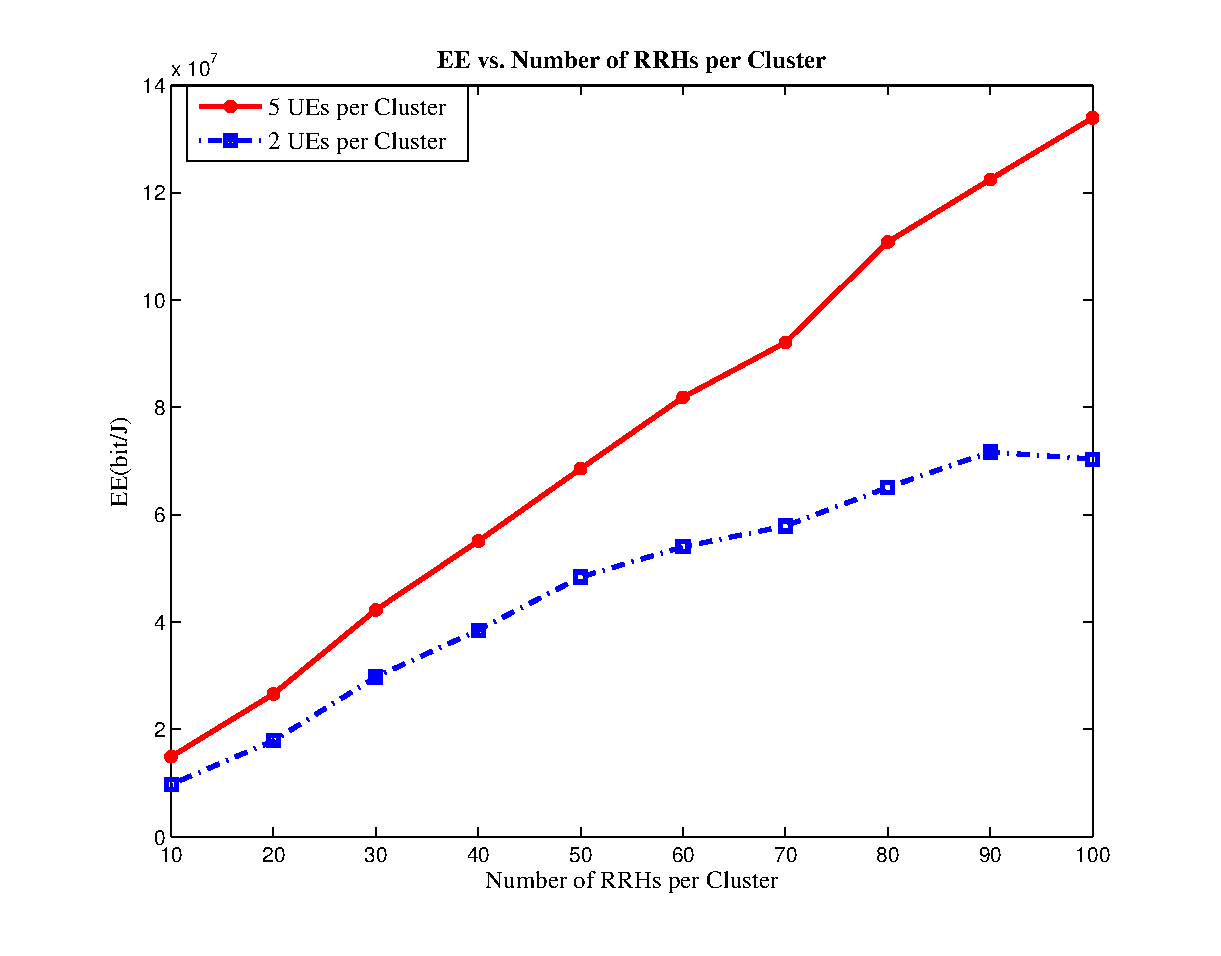
\includegraphics[width=\linewidth, height=12cm]{./fig3/rrh1}
  \caption{
  بازدهی انرژی با توجه به تغییرات تعداد واحدهای رادیویی  در هر خوشه برای توان بهینه برای 
   دو کاربر مختلف
   و پارامترهای جدول \ref{tab:title22}}
  \label{fig:nem1}
\end{figure}
 در شکل \ref{fig:nem1}، بازدهی انرژی سیستم \lr{MIMO C-RAN} بر اساس تعداد واحدهای رادیویی در هر خوشه برای مدل سیستم مورد نظر و برای دو تعداد کاربر متفاوت، رسم شده است. فرض اینجا بر این است که 2 خوشه برای لینک فروسو و دو خوشه برای فراسو وجود دارد.
 همانطور که  شکل  نشان می دهد، با افزایش تعداد واحدهای رادیوی، بازدهی انرژی افزایش می یابد زیرا  در اینجا با افزایش تعداد واحدهای رادیویی، مجموع توان کل افزایش می یابد در نتیجه نرخ انتقال داده نیز بیشتر می گردد و در نتیجه ی آن، بازدهی انرژی نیز افزایش یافته است. همچنین بازدهی انرژی برای تعداد کاربر بیشتر، به دلیل اینکه مجموع نرخ ها بیشتر می گردد، زیادتر می باشد.
 \begin{figure}[H]
  \centering
    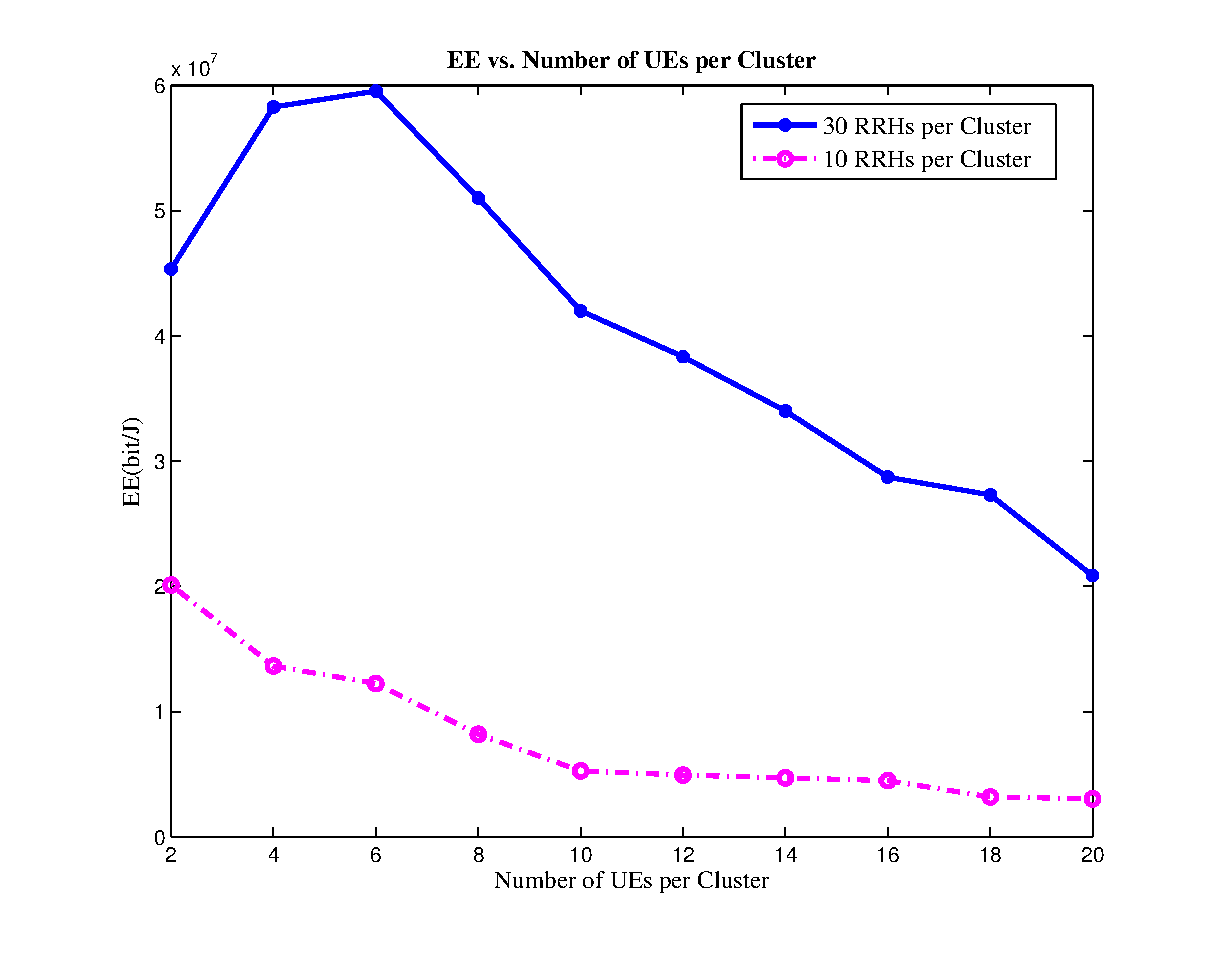
\includegraphics[width=\linewidth]{./fig3/ue4}
  \caption{  بازدهی انرژی با توجه به تغییرات تعداد کاربران در هر خوشه برای توان بهینه برای 
   دو واحد رادیویی مختلف
   و پارامترهای جدول
    \ref{tab:title22} }
  \label{fig:ue4}
\end{figure}

در شکل \ref{fig:ue4}، بازدهی انرژی بر اساس تعداد کاربران در هر خوشه برای مدل سیستم مورد نظر و برای دو تعداد واحد رادیویی متفاوت، رسم شده است. همانطور که  دیده می شود با افزایش تعداد کاربران، در حالتی که 30 واحد رادیویی در هر خوشه داریم، ابتدا به دلیل افزایش کاربران و افزایش مجموع نرخ ها، بازدهی انرژی زیاد شده و در نتیجه ی آن شیب نمودار زیاد می شود ولی از یک مقدار به بعد تداخل بین کاربران افزایش می یابد و منجر به کاهش بازدهی انرژی می گردد. زمانی که تعداد کاربران زیاد نیست، تداخل بین کاربران تاثیر کمی می گذارد و با افزایش کاربران بازدهی انرژی بهبود می یابد ولی زمانی که تعداد کاربران از حدی بیشتر می شود، میزان تداخل به قدری زیاد شده که نرخ انتقال داده کاهش یافته و در نتیجه ی آن، بازدهی انرژی کاهش می یابد. 
در حالتی که  10 واحد رادیویی در هر خوشه داریم، به دلیل اینکه میزان تداخل بین کاربران زیاد است و \lr{SINR} کم است، شیب نمودار از ابتدا منفی است و بازدهی انرژی کم می گردد.
 \begin{figure}[H]
  \centering
    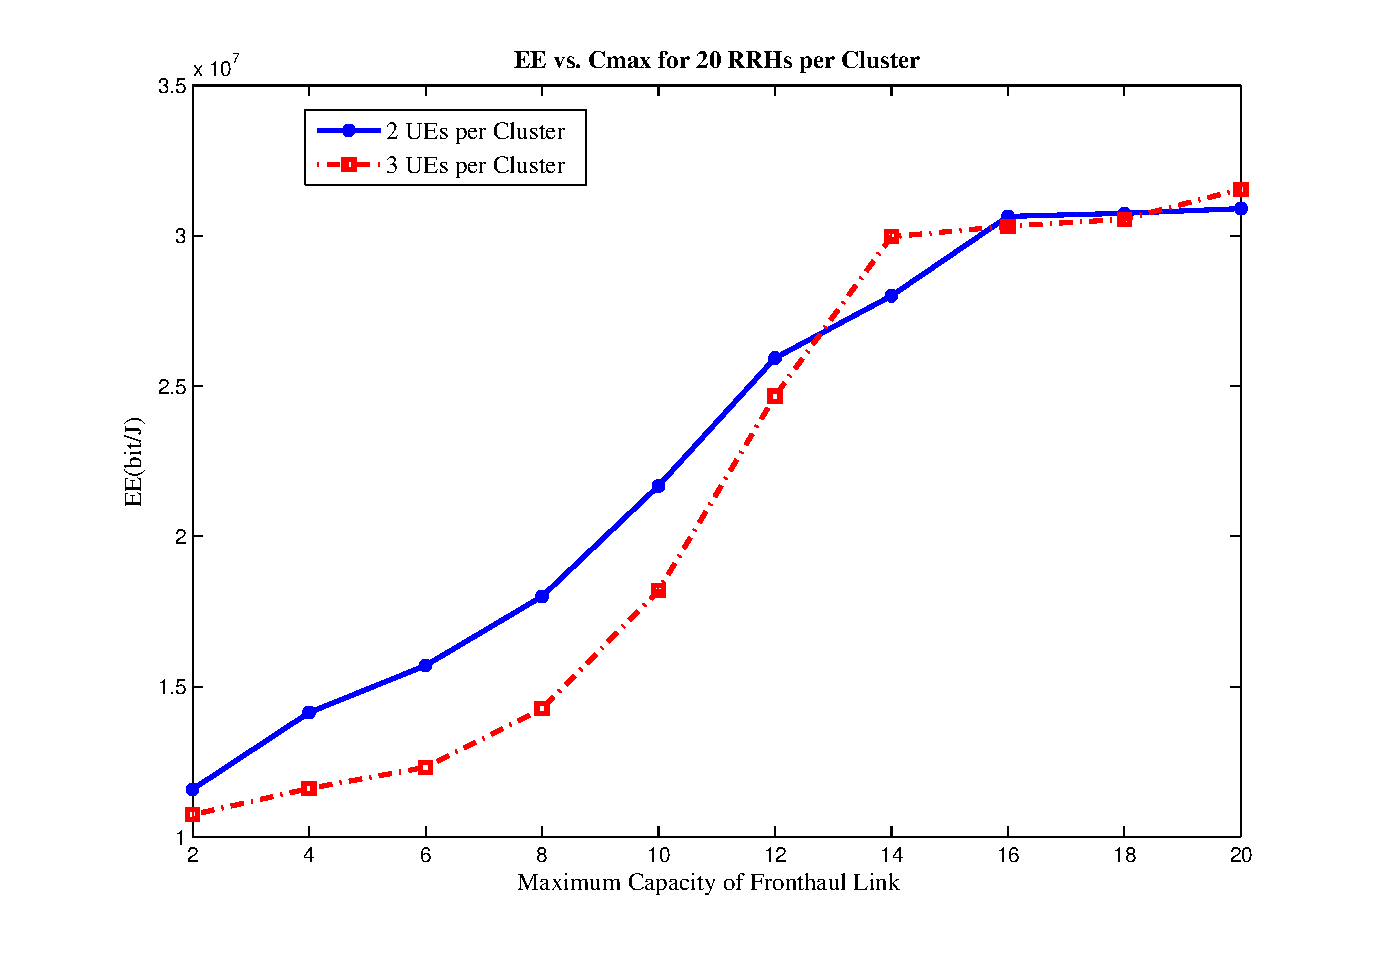
\includegraphics[width=\linewidth]{./fig3/c4}
  \caption{  
  بازدهی انرژی با توجه به تغییرات ظرفیت
   بیشینه ی لینک \lr{fronthaul}
   در هر خوشه برای توان بهینه برای 
   دو تعدا کاربر مختلف
   و پارامترهای جدول
    \ref{tab:title22} }
  \label{fig:c4}
\end{figure}
در شکل \ref{fig:c4}، بازدهی انرژی بر اساس تغییرات ظرفیت
   بیشینه ی لینک \lr{fronthaul} در هر خوشه برای مدل سیستم مورد نظر و برای دو تعداد کاربر متفاوت، رسم شده است.همانطور که  دیده می شود با افزایش این ظرفیت، بازدهی انرژی با شیب زیادی، افزایش یافته ولی از جایی به بعد شیب افزایش کم می گردد زیرا با افزایش بیشینه ی ظرفیت، تعداد بیت های بیشتری می تواند از این لینک عبور کند ولی از یک جایی به بعد، تعداد بیتهایی که در هر ثانیه وجود دارد از نرخ انتقال بیت کمتر است، پس با افزایش نرخ، بازدهی انرژی افزایش پیدا نمی کند. 
\section{نتیجه گیری}
در این فصل، مدل سیستم جدیدی که همزمان شامل چندین خوشه ی لینک فروسو و فراسو است، بیان شده است و همزمان مجموع نرخ های قابل دسترسی بر روی توان کل خوشه های لینک فراسو و فروسو بیشینه شده است و نمودارهای آن را بر حسب تعداد کاربران و واحدهای رادیویی رسم شده اند. با توجه به نمودارها، با افزایش تعداد واحدهای رادیویی توان ارسالی افزایش یافته و بازدهی انرژی بهبود می یابد.  همچنین با افزایش کاربران ابتدا بازدهی انرژی بهبود یافته زیرا مجموع توان افزایش می یابد ولی از حدی به بعد، تاثیر تداخل بین کاربران زیاد شده و بازدهی کاهش می یابد.

\chapter{ نتيجه‌گيري و پیشنهادات}
%%%%%%%%%%%%%%%%%%%%%%%%%%%%%%%%%%%%%%%%%%%
در این فصل، ابتدا مروری بر کارهای انجام شده صورت گرفته، سپس به جمع بندی و نتیجه گیری آنها پرداخته شده است. در نهایت پیشنهادات خود را برای کارهای آتی بیان نموده ایم.
\section{مروری بر کارهای صورت گرفته}
در این پروژه، ابتدا در فصل اول به بررسی ساختار سنتی ایستگاه پایه و واحد رادیویی پرداخته شده و سپس به دلیل نیاز به ساختاری جدید برای غلبه بر مشکلات آن، ساختار جدیدی به نام \lr{C-RAN} که پژوهشگران در حال پرداختن به آن هستند،بیان شده است. همچنین مزایا و معایب این ساختار جدید شرح داده شده و ساختارهای دیگر \lr{H-CRAN} و \lr{F-RAN} نیز در ادامه توضیح داده شده است. 

در فصل دوم یکی از چالش های این ساختار که در مقالات مختلف آورده شده، شرح داده شده است که در رابطه با تخصیص منابع در لینک فراسو و فروسو می باشد. در فصل سوم و چهارم نیز مدل سیستمهای جدیدی تشریح گردیده است که در ادامه خلاصه ای از آن شرح داده می شود. \\
در فصل سوم مدل سیستمی که شامل تعدادی خوشه است در نظر گرفته شده و همچنین ظرفیت لینک \lr{fronthaul} نیز محدود می باشد. در لینک فراسو و فروسو این مدل سیستم ارائه شده و  الگوریتم تخصیص منابع بر روی آن صورت گرفته شده است. 

در فصل چهارم مدل سیستم فصل سوم با فرض \lr{TDD} در نظر گرفته شده است. در این مدل سیستم چندین خوشه در لینک فروسو و چندین خوشه ی دیگر در همان زمان در لینک فراسو عمل می کنند. تداخل این دو دسته خوشه بر یکدیگر اثر می گذارد. حال تخصیص منابع به طور همزمان بر روی هر دو خوشه صورت می گیرد.
\section{نتیجه گیری}
با توجه به نمودارهای رسم شده در فصل های 2 و 3 و4، می توان فهمید که با افزایش تعداد واحدهای رادیویی، بازدهی انرژی بهبود می یابد. همچنین در مدل سیستم های گفته شده، پیش کدگذاری \lr{MMSE}
 بازدهی انرژی بیشتری نسبت به \lr{MRT}
 دارند.
علاوه بر این با افزایش تعداد کاربران، ابتدا به علت افزایش مجموع نرخ های قابل دسترس، بازدهی انرژی بیشتر شده و سپس به دلیل افزایش تداخل بین کاربران و محسوس شدن آن، بازدهی انرژی کاهش می یابد. 
همچنین می توان نتیجه گرفت که با افزایش بیشینه ی ظرفیت لینک \lr{fronthaul}، بازدهی انرژی افزایش پیدا می کند و سپس شیب افزایش بازدهی انرژی کم شده و در نهایت به مقدار خاصی میل می کند.
علاوه بر این، هر چه قدر نویز کوانتیزاسیون کمتر باشد، بازدهی انرژی بهتر می گردد زیرا با کاهش نویز کوانتیزاسیون، مقدار ظرفیت لینک \lr{fronthaul} بیشتر شده و خطای ناشی از فشرده سازی کمتر می شود و در نتیجه ی آن بازدهی انرژی بهبود می یابد.
\section{پیشنهادات}
در این بخش به بیان پیشنهادات برای کارهای آتی پرداخته شده است. یکی از کارهایی که در ادامه می توان انجام داد، تولید الگوریتم های بهینه سازی دیگر می باشد که منجر به بهبود بیشتر بازدهی انرژی می شود. همچنین الگوریتم های غیر محدب نیز می تواند مسیر بعدی این پروژه باشد. علاوه بر این مدل سیستم های \lr{D2D} نیز یکی دیگر از زمینه های کاری آتی می باشد که در راستای سیستم های \lr{F-RAN} است. به علاوه استفاده از روش های یادگیری ماشین در زمینه ی خوشه سازی نیز می تواند یکی از کارهای  آتی این پروژه باشد. همچنین می توان خوشه سازی و پیش کدگذاری و یا پرتو دهی را به طور همزمان با روش های تخصیص منابع برای فصل 4 انجام داد \cite{clusterbeam}. یکی دیگر از کارهای قابل انجام، این است که بتوان دریافت که به ازای هر کاربر چند واحد رادیویی نیاز است که بازدهی انرژی به بیشینه مقدار خود برسد و از آن تعداد واحد رادیویی به بعد، مقدار بازدهی انرژی تغییر چندانی نکند. همچنین می توان فصل چهارم را با روش \lr{ECF} \LTRfootnote{Esitimation-Compress and Forward} فشرده سازی کرد و با روش \lr{CFE} \LTRfootnote{Compress-Forward Estimation} مقایسه نمود \cite{ulSimeone}. 

%--------------------------------------------------------------------------appendix( مراجع و پیوست ها)
\chapterfont{\vspace*{-2em}\centering\LARGE}%

\appendix
%\bibliographystyle{plain-fa}
%\bibliographystyle{ieeetr}
%\bibliography{references}
\begin{latin}
\bibliographystyle{IEEEtran}
\renewcommand{\bibname}{\rl{{کتاب‌نامه}\hfill}} 
\bibliography{IEEEabrv,references}
\end{latin}
%\chapter*{‌پیوست}
موضوعات مرتبط با متن گزارش پایان نامه كه در يكی از گروه‌های زير قرار می‌گيرد، در بخش پيوست‌ها آورده شوند:
\begin{enumerate}
\item  اثبات های رياضی يا عمليات رياضی طولانی‌.‌
\item داده و اطلاعات نمونه (های) مورد مطالعه (\lr{Case Study}) چنانچه طولانی باشد‌.‌
\item نتايج كارهای ديگران چنانچه نياز به تفصيل باشد‌.‌

\item مجموعه تعاريف متغيرها و پارامترها، چنانچه طولانی بوده و در متن به انجام نرسيده باشد‌.‌
\end{enumerate}
% براي شماره‌گذاري روابط، جداول و اشكال موجود در پيوست‌ از ساختار متفاوتي نسبت به متن اصلي استفاده مي‌شود كه در زير به‌عنوان نمونه نمايش داده شده‌است. 
% \begin{equation}
%F=ma
%\end{equation}
\section*{کد میپل }
\begin{latin}
\begin{verbatim}

with(DifferentialGeometry):
with(Tensor):
DGsetup([x, y, z], M)
																	frame name: M
a := evalDG(D_x)
																	D_x
b := evalDG(-2 y z D_x+2 x D_y/z^3-D_z/z^2)


\end{verbatim}
\end{latin}
%--------------------------------------------------------------------------dictionary(واژه نامه ها)
%اگر مایل به داشتن صفحه واژه‌نامه نیستید، خط زیر را غیر فعال کنید.
%\parindent=0pt
%%
\chapter*{واژه‌نامه‌ی فارسی به انگلیسی}
\pagestyle{style9}

\addcontentsline{toc}{chapter}{واژه‌نامه‌ی فارسی به انگلیسی}
%%%%%%
\begin{multicols*}{2}

{\bf آ}
\vspace*{3mm}


\farsiTOenglish{اسکالر}{Scalar}


\vspace*{3mm}
{\bf ب}
\vspace*{3mm}

\farsiTOenglish{بالابر}{Lift}


\vspace*{3mm}
{\bf پ}
%%\vspace*{3mm}

\farsiTOenglish{پایا}{Invariant}



\vspace*{3mm}
{\bf ت}
%%\vspace*{3mm}

\farsiTOenglish{ تناظر }{Correspondence}


\vspace*{3mm}
{\bf ث}
%%\vspace*{3mm}

\farsiTOenglish{ثابت‌ساز}{Stabilizer}

\vspace*{3mm}
{\bf ج}
%%\vspace*{3mm}

\farsiTOenglish{جایگشت}{Permutation}



\vspace*{3mm}
{\bf چ}
%%\vspace*{3mm}


\farsiTOenglish{چند جمله‌ای }{Polynomial}

\vspace*{3mm}
{\bf ح}
%%\vspace*{3mm}

\farsiTOenglish{حاصل‌ضرب دکارتی}{Cartesian product}


\vspace*{3mm}
{\bf خ}
%%\vspace*{3mm}

\farsiTOenglish{خودریختی}{Automorphism}

\vspace*{3mm}
{\bf د}
%%\vspace*{3mm}

\farsiTOenglish{درجه}{Degree}


\vspace*{3mm}
{\bf ر}
%%\vspace*{3mm}


\farsiTOenglish{ریزپردازنده}{microprocessor}


\vspace*{3mm}
{\bf ز}
%%\vspace*{3mm}


\farsiTOenglish{زیرمدول}{Submodule}


\vspace*{3mm}
{\bf س}
%%\vspace*{3mm}

\farsiTOenglish{سرشت}{Character}


\vspace*{3mm}
{\bf ص}
%%\vspace*{3mm}

\farsiTOenglish{صادقانه}{Faithful}

\vspace*{3mm}
{\bf ض}
%%\vspace*{3mm}

\farsiTOenglish{ضرب داخلی}{Inner product}

\vspace*{3mm}
{\bf ط}
%%\vspace*{3mm}


\farsiTOenglish{طوقه}{Loop}


\vspace*{3mm}
{\bf ظ}
%%\vspace*{3mm}


\farsiTOenglish{ظرفیت}{Valency}
 
\vspace*{3mm}
{\bf ع}
%%\vspace*{3mm}


\farsiTOenglish{عدم مجاورت}{Nonadjacency}



\vspace*{3mm}
{\bf ف}
%%\vspace*{3mm}

\farsiTOenglish{فضای برداری}{Vector space}



\vspace*{3mm}
{\bf ک}
%%\vspace*{3mm}

\farsiTOenglish{کاملاً تحویل‌پذیر}{Complete reducibility}


\vspace*{3mm}
{\bf گ}
%%\vspace*{3mm}


\farsiTOenglish{گراف}{Graph}



\vspace*{3mm}
{\bf م}
%%\vspace*{3mm}

\farsiTOenglish{ماتریس جایگشتی}{Permutation matrix }


\vspace*{3mm}
{\bf ن}
%%\vspace*{3mm}

\farsiTOenglish{ناهمبند}{Disconnected}


\vspace*{3mm}
{\bf و}
%%\vspace*{3mm}

\farsiTOenglish{وارون‌پذیر}{Invertible}


\vspace*{3mm}
{\bf ه}
%%\vspace*{3mm}

\farsiTOenglish{همبند}{Connected}



\vspace*{3mm}
{\bf ی}
%%\vspace*{3mm}

\farsiTOenglish{یال}{Edge}




\end{multicols*}%
%%%%%%%
\chapter*{ واژه‌نامه‌ی انگلیسی به فارسی}
\pagestyle{style9}
\lhead{\thepage}\rhead{واژه‌نامه‌ی انگلیسی به فارسی}
\addcontentsline{toc}{chapter}{واژه‌نامه‌ی انگلیسی به فارسی}

\LTRmulticolcolumns
\begin{multicols}{2}

{\hfill\bf  \lr{A}}
%%\vspace*{1.5mm}


\englishTOfarsi{Automorphism}{خودریختی}


\vspace*{3mm}
{\hfill\bf   \lr{B}}
%%\vspace*{1.5mm}


\englishTOfarsi{Bijection}{دوسویی}


\vspace*{3mm}
{\hfill\bf   \lr{C}}
%%\vspace*{1.5mm}


\englishTOfarsi{Cycle group}{گروه دوری}

\vspace*{3mm}
{\hfill\bf   \lr{D}}
%%\vspace*{1.5mm}

\englishTOfarsi{Degree}{درجه}


\vspace*{3mm}
{\hfill\bf   \lr{E}}
%%\vspace*{1.5mm}

\englishTOfarsi{Edge}{یال}



\vspace*{3mm}
{\hfill\bf   \lr{F}}
%%\vspace*{1.5mm}


\englishTOfarsi{Function}{تابع}


\vspace*{3mm}
{\hfill\bf   \lr{G}}
%%\vspace*{1.5mm}


\englishTOfarsi{Group}{گروه}

\vspace*{3mm}
{\hfill\bf   \lr{H}}
%%\vspace*{1.5mm}

\englishTOfarsi{Homomorphism}{همریختی}


\vspace*{3mm}
{\hfill\bf   \lr{I}}
%%\vspace*{1.5mm}


\englishTOfarsi{Invariant}{پایا}


\vspace*{3mm}
{\hfill\bf   \lr{L}}
%%\vspace*{1.5mm}

\englishTOfarsi{Lift}{بالابر}



\vspace*{3mm}
{\hfill\bf   \lr{M}}
%%\vspace*{1.5mm}


\englishTOfarsi{Module}{مدول}



\vspace*{3mm}
{\hfill\bf   \lr{N}}
%%\vspace*{1.5mm}

\englishTOfarsi{Natural map}{نگاشت طبیعی}


\vspace*{3mm}
{\hfill\bf   \lr{O}}
%%\vspace*{1.5mm}


\englishTOfarsi{One to One}{یک به یک}



 \vspace*{3mm}
{\hfill\bf   \lr{P}}
%%\vspace*{1.5mm}


\englishTOfarsi{Permutation group}{گروه جایگشتی}


\vspace*{3mm}
{\hfill\bf   \lr{Q}}
%%\vspace*{1.5mm}

\englishTOfarsi{Quotient graph}{گراف خارج‌قسمتی}

 \vspace*{3mm}
{\hfill\bf   \lr{R}}
%%\vspace*{1.5mm}

\englishTOfarsi{Reducible}{تحویل پذیر}


 \vspace*{3mm}
{\hfill\bf   \lr{S}}
%%\vspace*{1.5mm}


\englishTOfarsi{Sequence}{دنباله}



 \vspace*{3mm}
{\hfill\bf   \lr{T}}
%%\vspace*{1.5mm}


\englishTOfarsi{Trivial character}{سرشت بدیهی}


\vspace*{3mm}
{\hfill\bf   \lr{U}}
%%\vspace*{1.5mm}

\englishTOfarsi{Unique}{منحصربفرد}


\vspace*{3mm}
{\hfill\bf   \lr{V}}
%%\vspace*{1.5mm}

\englishTOfarsi{Vector space}{فضای برداری}



\end{multicols}
%--------------------------------------------------------------------------index(نمایه)
%اگر مایل به داشتن صفحه نمایه نیستید، خط زیر را غیر فعال کنید.
\pagestyle{style7}
\printindex
\pagestyle{style7}
%کلمات کلیدی انگلیسی
\latinkeywords{ Cloud Radio Access Network, Multiple-Input Multiple-Output, Energy efficiency, Clusterization, Power allocation, Lagrangian function.}
%چکیده انگلیسی

\en-abstract{
Since more rate and speed is needed in technology, new generation of technology is considered that new concepts such as CRAN, mm wave, Massive MIMO and etc are defined. 
Cloud radio access networks generate a new architechture for 5G that is proposed to enhance both spectral efficiency and energy efficiency. 
The architecture of cran and the difference between this architucture and traditional one is expressed.
Also some system models such as clustering and limited fronthaul capacity is considered. In addition, D2D system in C-RAN is described too.
The optimal power allocation for the downlink and uplink of Multiple-Input Multiple-Output (MIMO) Cloud Radio Access Network (C-RAN) with limited fronthaul capacity in terms of maximizing Energy Efficiency (EE) is investigated. 
In the considered system, in downlink the compressed and precoded message generated by Central Unit (CU) is transmitted to Remote Radio Heads (RRHs) via a fronthaul link with limited capacity, and the RRHs and Users Equipments (UEs) are assumed to be clustered into $S$ cluster sets.
In uplink, the recieved message by RRHs which are clusteres into $S$ clusters, is transmitted through fronthaul link to CU and in CU beamforming vector is applied to the message.
Here, we use an iterative algorithm with Lagrangian function to optimize the EE.
Also both uplink and downlink clusters are considered in a system model and optimization is done for both together.
}
%%%%%%%%%%%%%%%%%%%%% کدهای زیر را تغییر ندهید.

\newpage
\thispagestyle{empty}
\begin{latin}
\section*{\LARGE\centering Abstract}

\een-abstract

\vspace*{.5cm}
{\large\textbf{Key Words:}}\par
\vspace*{.5cm}
\elatinkeywords
\end{latin}
% در این فایل، عنوان پایان‌نامه، مشخصات خود و چکیده پایان‌نامه را به انگلیسی، وارد کنید.
%%%%%%%%%%%%%%%%%%%%%%%%%%%%%%%%%%%%
\baselineskip=.6cm
\begin{latin}

\latinfaculty{Department of Electrical Engineering}


\latintitle{Improveing the performance of Cloud Radio Access Network with distributed cooperation}


\firstlatinsupervisor{Dr. Mohammad Javad Emadi}

%\secondlatinsupervisor{Second Supervisor}

\firstlatinadvisor{Dr. Abbas Mohammadi }

%\secondlatinadvisor{Second Advisor}

\latinname{Mojdeh}

\latinsurname{Karbalaee Motalleb}

\latinthesisdate{Month 6 \& Year 1396}

\latinvtitle
\end{latin}

\end{document}